\documentclass[12pt,PhD,wordcount,anon]{muthesis}
% The regulations say that 12pt should be used
% Change the MSc option to MPhil, MRes or PhD if appropriate

\usepackage{verbatim}
\usepackage{graphicx}
\usepackage{url} % typeset URL's reasonably
\usepackage{listings}
\usepackage{pslatex} % Use Postscript fonts
\usepackage{amsmath}
\usepackage{amssymb}
\usepackage{enumitem}

% Uncomment the next line if you want subsubsections to be numbered
%\setcounter{secnumdepth}{3}
% Uncomment the next line if you want subsubsections to be appear in
% the table of contents
%\setcounter{tocdepth}{3}

% Uncomment the following lines if you want to include the date as a
% header in draft versions
%\usepackage{fancyhdr}
%\pagestyle{fancy}
%\lhead{}  % left head
%\chead{Draft: \today} % centre head
%\lfoot{}
%\cfoot{\thepage}
%\rfoot{}

\begin{document}
% Uncomment the following lines to leave out list of figures, tables
% and copyright until final printing
%\figurespagefalse
%\tablespagefalse
%\copyrightfalse

\title{Surrogate Machine Learning Model Development for the UK Nuclear Industry}
\author{Huw Rhys Jones}
\stuid{10433506}
\principaladviser{Tingting Mu}

\beforeabstract

\prefacesection{Abstract}
% Single spacing can be turned on for the abstract
%
{
	
	\singlespacing
	This thesis details the development of machine learning techniques for the benefit of safety analysis in the UK nuclear energy sector. The objective of this research was to develop machine learning models which can perform the same functionality as existing industry standard models but with reduced computational intensity.  
	
	\singlespacing
	The UK nuclear industry is dominated by the advanced-gas cooled reactor (AGR), a design which differs considerably to most reactors elsewhere in the world. As a result of its novelty, there is a lack of international research to draw on concerning operation and safety. The situation is further complicated by the complexity of AGR safety analysis, involving thousands of different components in various scenarios and configurations. Therefore, AGR safety analysis and research is computationally intensive whilst being highly time sensitive.
	
	\singlespacing
	A key research objective was the production of surrogate machine learning (SML) models. These models are produced intention of retaining the functionality of an existing model i.e. it produces similar outputs from the same inputs whilst reducing computational cost.
	
	\singlespacing
	Through the development of SMLs for this research work, two articles were written and published in peer-reviewed academic journals. The first details the generation and preparation of data, as well as the process of developing an SML for our purpose. The second article details improvements to the method outlined in the first article. 
	


}



\afterabstract

\prefacesection{Acknowledgements}
I would like to thank my supervisor, Tingting Mu, who spent many patient hours with me throughout my journey towards becoming a researcher. I'd also like to thank many other members of the faculty for their help and support over the past four years, including Professor Gavin Brown, Professor Bijan Parsia, Dr Danny Wood, Charlie Reynolds, Dr Andrew Webb, Dr Alessio Sarullo and Dr Mike Phuycharoen. 
\\

\noindent
I'd also like to acknowledge the assistance
given by Research IT and the use of the Computational
Shared Facility at The University of Manchester.
\\

\noindent
Finally I'd like to thank my mother Tula Jones and my late father Tudor Jones for their love and unending support, not only during my PhD but my whole life.
\afterpreface

% These include the actual text
\chapter{Introduction}
\label{cha:intro}

\section{Outline}


The overarching motivation behind this thesis is to develop machine learning (ML) techniques for the benefit of safety analysis in the UK nuclear energy sector. The objective of this research was to develop machine learning models which can perform the same functionality as existing industry standard models but with reduced computational intensity.  
\\ 

\noindent
The UK nuclear industry is dominated by the advanced-gas cooled reactor (AGR), a design which uses graphite as a structural component and carbon dioxide gas as a coolant. The AGR differs in design to most reactors elsewhere in the world, meaning there is a lack of international research to draw on concerning operation and safety. Instead, all analysis must be preformed domestically, meaning that research in this field is intensive. The situation is further complicated by the complexity of AGR safety analysis, involving thousands of different components in various scenarios and configurations. The combination of these factors means that those responsible for demonstrating the safety of AGR reactors face challenges in terms of computational requirements whilst having a time sensitive task. 
\\ 

\noindent
The research question to be answered in this thesis concerns whether the difficulties faced within the UK nuclear industry can be alleviated through the use of machine learning techniques. To this end, a key research objective is the production of surrogate machine learning models (SMLMs). SMLMs are produced with the intention of retaining the functionality of an existing model i.e. it produces similar outputs from the same inputs. The intended advantage of SMLMs over the models they surrogate is low computational cost, hence fast inference of outputs from inputs. Compared to the original models, which may take many hours or even days to complete their analysis, SMLMs once trained can produce outputs in seconds using the same computational hardware. 
\\ 

\noindent
Through the development of SMLMs for this research work, two articles were written and published in peer-reviewed academic journals. The first article, presented in the journal of Nuclear Engineering and Design, details the generation and preparation of data, as well as the process of developing an SML for our purpose. This article highlights how some methods were found to be highly effective, such as convolutional neural networks and regularisation. It was noted that through a process of feature selection, not only can performance of the model be improved, but insights into the underlying nature of the data space can be observed. The second article, presented in IEEE Access, details improvements to the method outlined in the first article. Three methods were exploited: data augmentation, custom loss functions and transfer learning. Each of these methods have seen previous exploitation within the field of machine learning, however, we implement them here in a novel way. 


\section{Research Objectives}

The key objectives of this research project are as follows.

\begin{enumerate}
	\item \textbf{Development and Optmisation of SMLMs} The overarching objective is to produce a machine learning model which surrogates the function of an existing standard engineering model. The aim is to reduce computational intensity whilst retaining a high level of accuracy/functionality. 
	
	\item \textbf{Data Visualisation Tools} With the data space for this research area being highly complex and multi-dimensional, a secondary objective is to explore the data through visualisation techniques. To this end, bespoke computational tools will need to be produced. The benefit of data visualisation for this research task is two fold: 1) It will help inform the process of machine learning model development and optimisation 2) Insights into the data space will be informative to a wider engineering audience.
	
	\item \textbf{Data Insights Through ML} Through the process of development and optimisation of SMLMs, insights into the underlying nature of the data space itself. These insights will benefit the development of SMLMs but also have value in and of itself. For example, relationships between parts of the data may yield insights which are useful from a wider engineering or safety perspective. 
	
	
\end{enumerate}

\section{Outcomes and Findings}

The key outcomes of this research project are as follows.

\begin{enumerate}
	\item \textbf{Identification of Effective ML techniques}
	Through development and optimisation of SMLMs for the research problem discussed in this thesis, we identified several techniques that were  highly effective in terms of model performance. Early in the development process, convolutional neural networks (CNNs) were identified as performing better than fully dense neural networks (DNNs). An unconventional alternating arrangement of activation functions was found to produce optimal model performance. Many other model parameters were optimised during the model development process which are detailed throughout this thesis.
	
	
	\item \textbf{Data Insights Through Visualisation} Through visualisation and analysis of the dataset we were able to better guide the direction of the research. This included selection of model inputs, outputs and the type of machine learning model to use.
	
	
	\item \textbf{SML Development Framework}  To aid in the development, optimisation and evaluation of SMLMs, a programmatic framework was developed. This framework streamlined the production of training data, data engineering, model parameter selection, training, optimisation and evaluation. The framework was produced using the programming language Python and using the Keras library. It is provided in an open source online repository with the intention that other researchers can adapt it to their own SMLM development work.
	 
	\item \textbf{Data Insights Through ML Model Optimisation}
	The process of SMLM optimisation not only enhanced model performance, but helped identify relationships and insights about the data itself. For example, the process of feature selection (identifying selected inputs which provide the best model performance), it was discovered that only including inputs representing the top three levels of the AGR core was optimal in output accuracy. This suggests that inputs concerning the lower levels of the core are irrelevant to the prediction of the output.  
	
	\item \textbf{Adaption of Existing ML techniques to SMLMs}
	To improve model performance and compensate for a lack of training data, several existing machine learning techniques were adapted from other research to serve the purpose of this project. For example, data augmentation, a technique widely used in image classification, was adapted to the regression problem discussed here. A bespoke machine learning loss function was also developed to better fit the data distribution. 
	
	
\end{enumerate}

\section{Thesis Structure}

The content of this thesis is presented as follows:

\begin{enumerate} 
	
	\item \textbf{Nuclear Engineering Background} Technical information concerning the AGR, traditional engineering calculations, existing modelling techniques. 
	
	\item \textbf{Machine Learning Background} Details of machine learning techniques and how they work. Differences between various methods.
	
	\item \textbf{Dataset Framework, Exploration and Analysis} Details of the programmatic dataset framework, as well as an exploration of the dataset using visualisation techniques and statistical methods.
	
	\item \textbf{Preliminary Machine Learning Experiments} Initial experiments performed with the intention of exploring the problem space and testing ideas. 
	
	\item \textbf{Development and Analysis of a Surrogate Machine Learning Model} This chapter is based on a published research paper of the same name. It covers the development and optimisation of a surrogate machine learning model. 
	
	\item \textbf{Methods to Improve Surrogate Machine Learning Model Performance} This chapter is based on another published work titled "Data-driven Approaches to Surrogate Machine Learning Model Development". It covers the adaption of existing machine learning methods to the research topic at hand.
		
\end{enumerate}
	
	



\chapter{Nuclear Engineering Background}
\label{cha:engineering}

\section{Advanced Gas-cooled Reactors (AGRs)} \label{AGR}

The UK nuclear power sector is dominated by the advanced gas-cooled reactor  (AGR) \cite{nonbol1996description}. There are 14 AGR reactors spread across 7 UK power stations . This design differs from most reactors around the world in that it consists of a graphite core cooled by carbon dioxide gas (as opposed to the common water cooled reactor). The international novelty of this design means that all safety analysis has to be performed domestically, leading to a significant requirement for computation.

\begin{figure}[ht!]
	\centering
	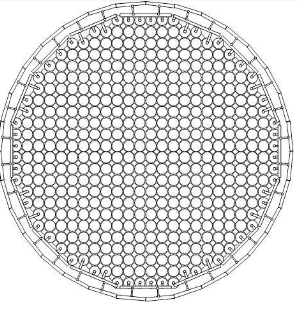
\includegraphics[scale=0.75]{Figures/AGR_plan.png}
	\caption{AGR Core Plan View}
	\label{fig:schematic}
\end{figure}

\noindent
The AGR consists of several thousand stacked graphite bricks assembled in an interlocking 3-dimensional assembly (shown in Figure~\ref{fig:schematic} and \ref{fig:side}). There are two principal brick types shown in Figure~\ref{fig:bricks}: (1) large bore bricks for the insertion of fuel assemblies and (2) interstitial bricks which provide structural support, some of which have a small bore to allow the insertion of a control rod. The bricks are linked and held in position by rectangular graphite keys. An individual stack of bricks the height of the core is known as a channel, with types of channel dictated by the type of brick i.e. fuel, control rod, filler, peripheral (fuel channels near the edge of the core) and reflector (the shape of fuel bricks but contain no fuel and are solid) channels. 

\begin{figure}[ht!]
	\centering
	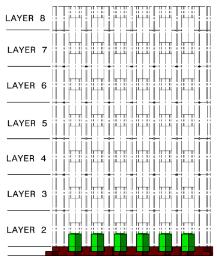
\includegraphics[scale=0.75]{Figures/AGR_side}
	\caption{AGR Core Side View}
	\label{fig:side}
\end{figure}

\noindent
The primary safety concern with the AGR is the cracking of the fuel bricks. Given enough cracks, the ability to insert fuel or control rods could be impeded. The mechanism by which the cracks occur is well understood. The intense heat and radiation cause a reduction in the mass and volume of the bricks, resulting in a stress differential, which leads to a concentration of stress and cracking at the root of the keyways (Figure \ref{fig:cracking}). \\ 

\noindent
The growth of these cracks ultimately results in the splitting of the brick into two halves (see Figure \ref{fig:cracked}). At any given time, it is difficult to ascertain which bricks are exhibiting cracks due to inaccessible nature of the core internals. Forecasting the location of cracks as a function of time is an area of ongoing research. Future inspection regimes may yield better information about where cracks are occurring.

\section{Traditional Engineering Safety Assessments} \label{Engineering}
The UK Office for Nuclear Regulation (ONR) stipulates that the AGR operator (EDF Energy) must demonstrate that the ability to control the reactor (i.e. insert control rods) will not be threatened under any circumstance i.e an earthquake or other serious event.\\

\begin{figure}[ht!]
	\centering
	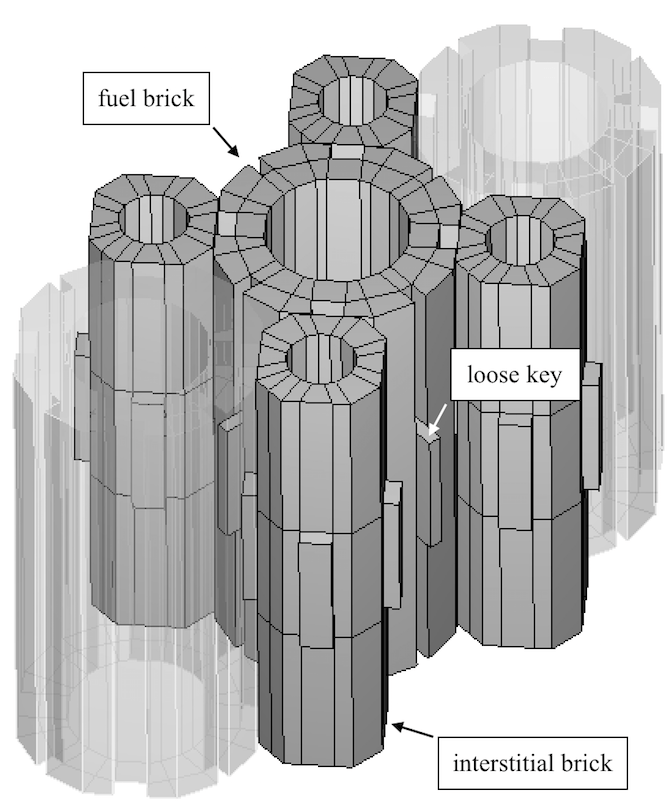
\includegraphics[scale=0.17]{Figures/brick_types_parmec}
	\caption{AGR Core Brick Types}
	\label{fig:bricks}
\end{figure}

\begin{figure}[ht!]
	\centering
	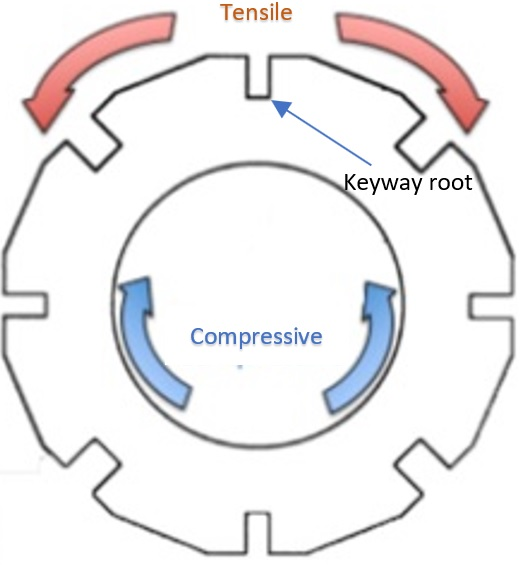
\includegraphics[scale=0.35]{Figures/cracking_mechanism}
	\caption{Brick Cracking Mechanism}
	\label{fig:cracking}
\end{figure}

\begin{figure}[ht!]
	\centering
	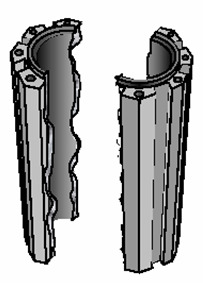
\includegraphics[scale=0.65]{Figures/Brick_Cracking}
	\caption{Cracked AGR Brick}
	\label{fig:cracked}
\end{figure}

\begin{figure}[b!]
	\centering
	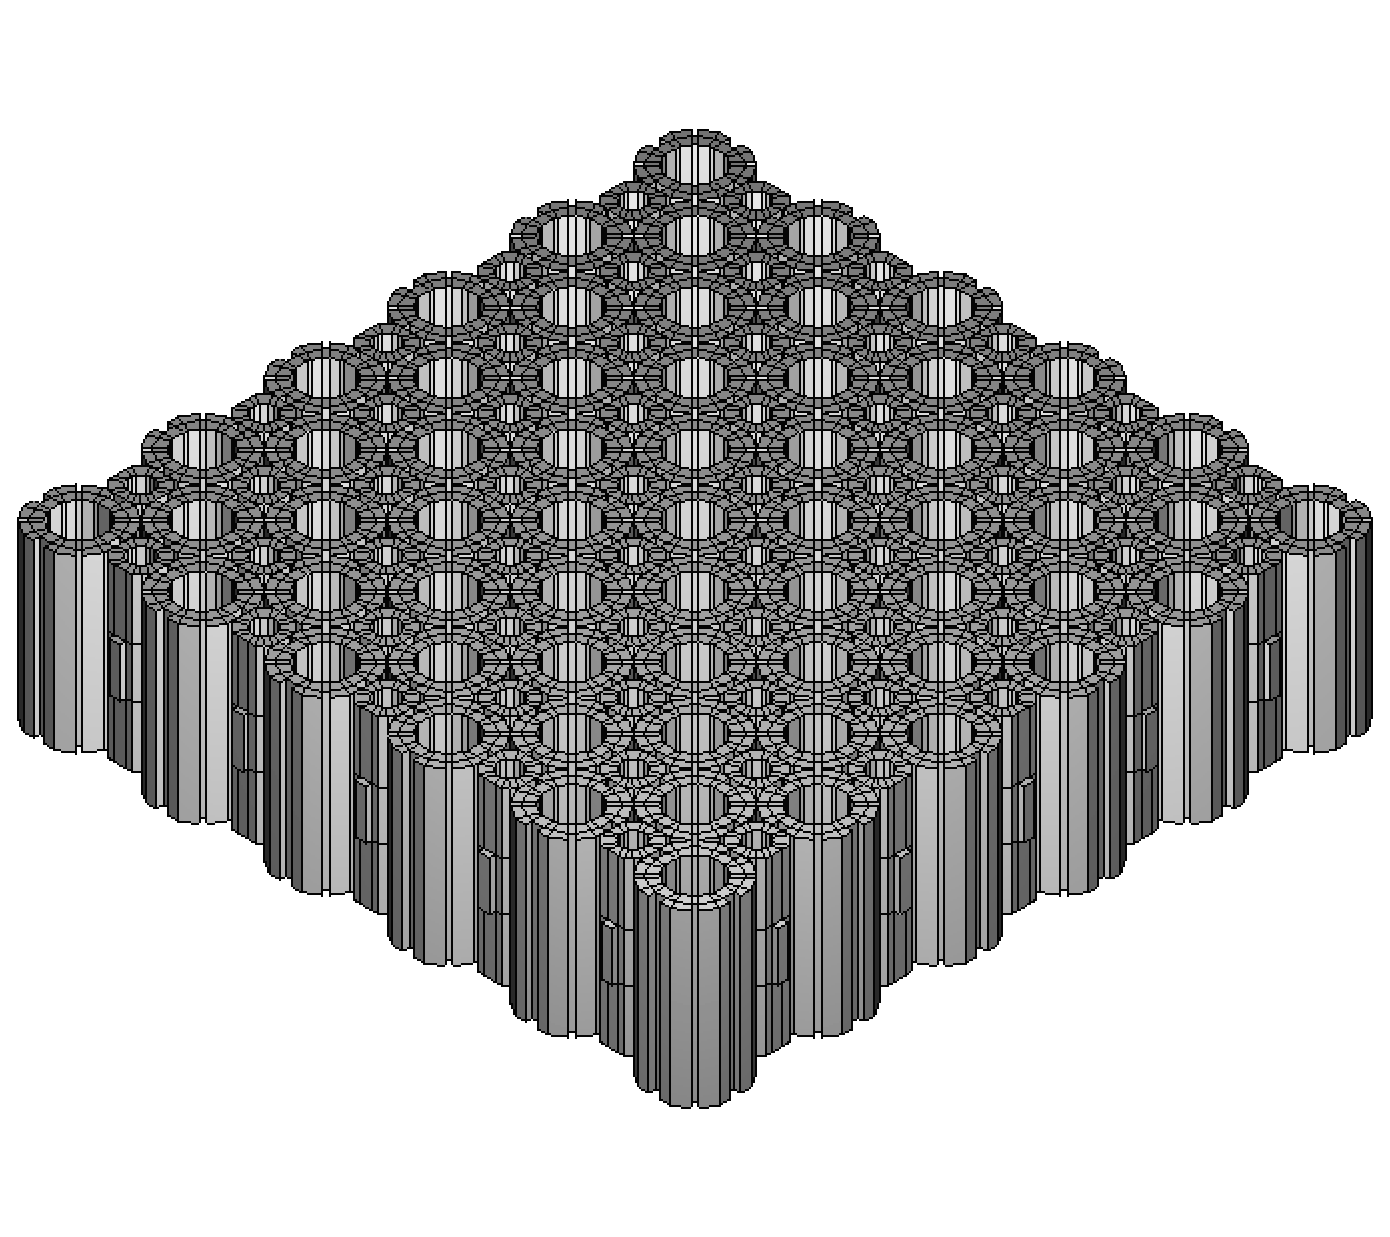
\includegraphics[scale=0.12]{Figures/parmec_bricks.png}
	\caption{Visualisation of Parmec Model}
	\label{fig:FEA}
\end{figure}

\noindent
The traditional approach used to ensure the safe condition of the AGR involves production and analysis of complex engineering models, which are deterministic and rely on physical relationships. Examples include the computational model Parmec \cite{wiki:xxx} and the physical Multi-Layer Array (MLA) model \cite{dihoru2014multi} at the University of Bristol (Figures \ref{fig:FEA} \& \ref{fig:ENG}, respectively). Both of these models are configured to to simulate a once in 10,000 year earthquake. \\

\begin{figure}[b!]
	\centering
	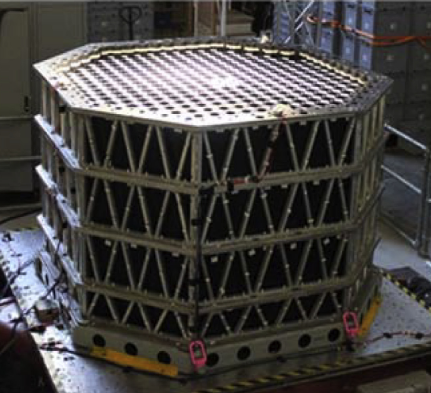
\includegraphics[scale=0.5]{Figures/MLA_rig}
	\caption{Multi-Layer Array Rig}
	\label{fig:ENG}
\end{figure}

\noindent
As mentioned at the end of section~\ref{AGR}, it is difficult to ascertain where the cracks are (or where they will occur). In lieu of actual crack positions, the traditional approach is to generate a random distribution of cracks, represented by a 3-dimensional array as shown in Figure~\ref{fig:core_array}. This array constitutes the structure of the AGR core, with the position of each element corresponding to a spatial position of a brick. This array has an integer data-type: -1 is an intact brick, 0 represents a reflector brick and 1~-~4 representing crack orientations - see Figure~\ref{fig:orientations}. \\

\begin{figure}[ht!]
	\centering
	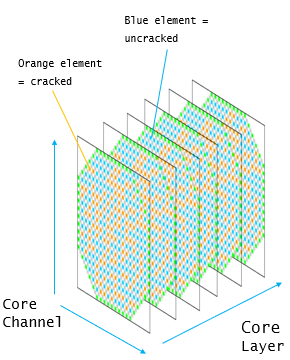
\includegraphics[scale=0.5]{Figures/core_array.png}
	\caption{AGR Input Core Array}
	\label{fig:core_array}
\end{figure}

\begin{figure}[ht!]
	\centering
	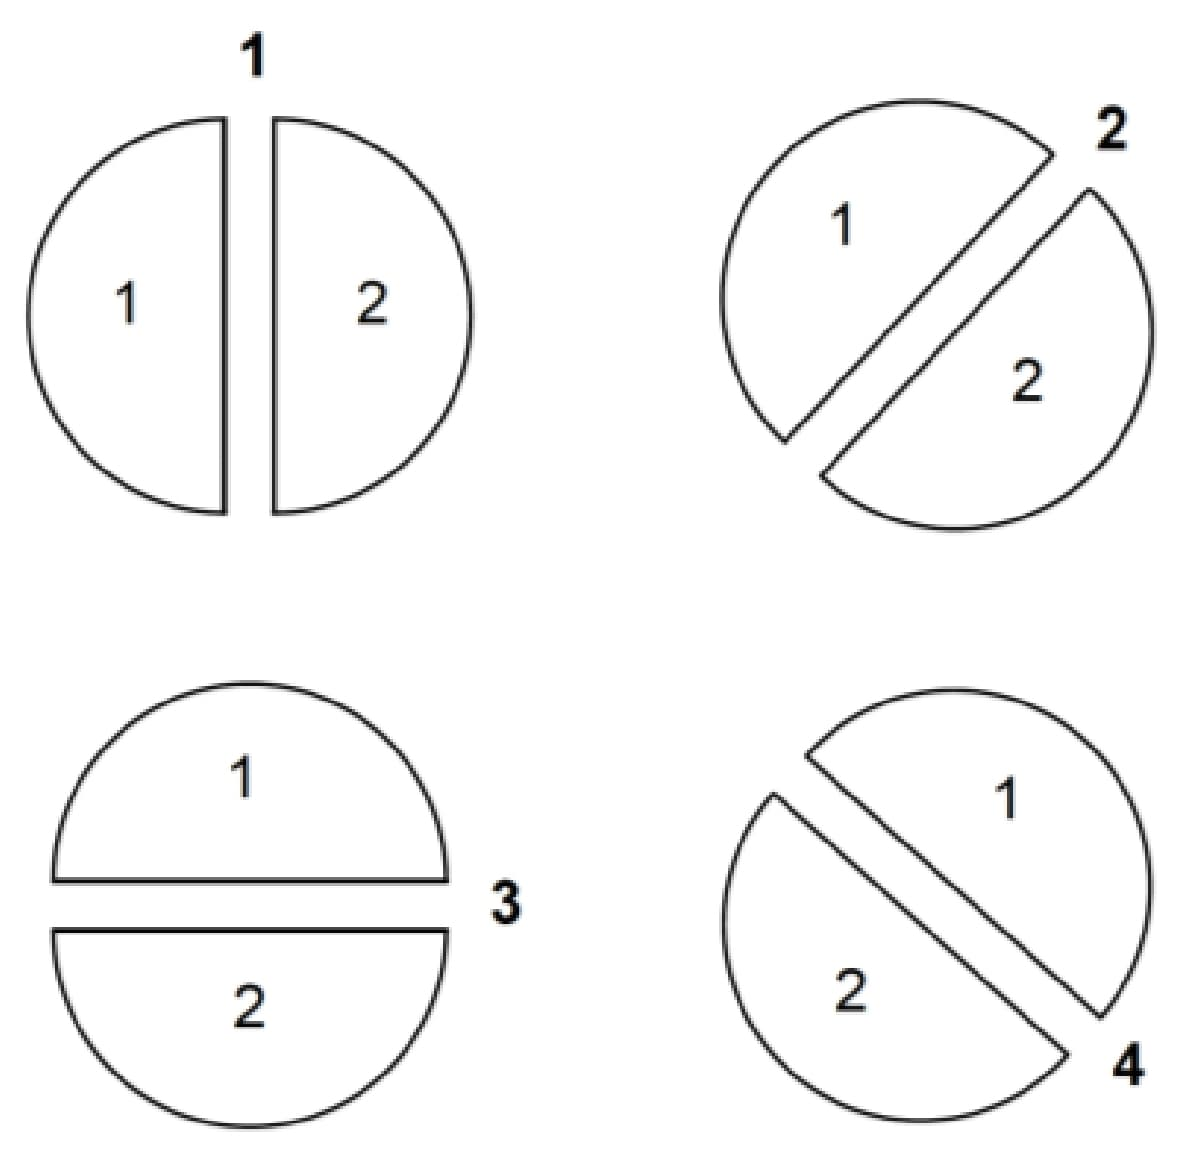
\includegraphics[scale=0.1]{Figures/orientations}
	\caption{Brick Crack Orientations}
	\label{fig:orientations}
\end{figure}

\noindent
The example array shown in Figure~\ref{fig:core_array} can be generated quickly and with low computational cost using industry standard tools (usually less than 1 minute per instance). These arrays can be used as input configurations to engineering models such as those shown in Figure~\ref{fig:FEA}~or~Figure~\ref{fig:ENG}. \\

\begin{figure}[ht!]
	\centering
	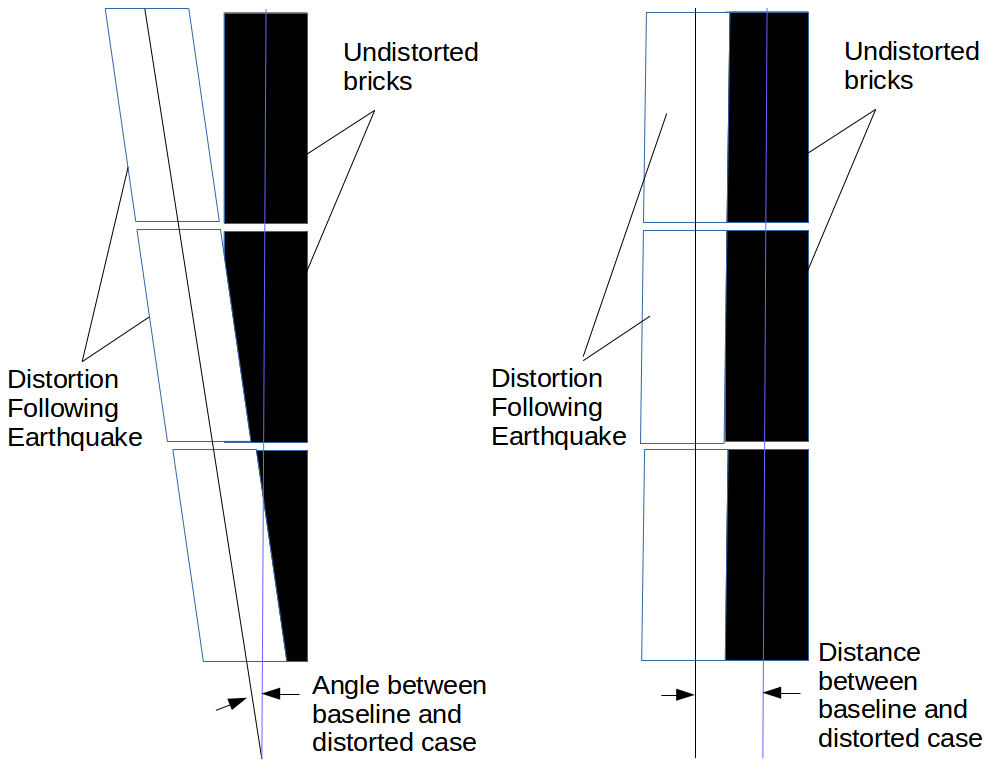
\includegraphics[scale=0.2]{Figures/Distored_bricks}
	\caption{Angle Between a Distorted and Baseline Brick Channel }
	\label{fig:angles}
\end{figure}

% 2D array
% Statistical Analysis

\noindent
The models are able to calculate the position of the bricks following an earthquake (Figure~\ref{fig:angles}) with the presence of cracked bricks influencing how the they move. Angular or translational movement of the bricks acts to effectively reduce the clearance between the fuel or control rod and the surrounding bore wall. Figure~\ref{fig:bore_clearance} illustrates an example involving a control rod channel: the relative displacement of the control rod insertion point can be calculated as a function of the movement of the bricks. The path of the control rod must not be obstructed, and so the relative displacement must be less than the bore radius. \\

\begin{figure}[ht!]
	\centering
	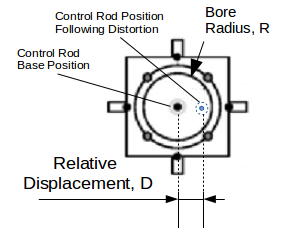
\includegraphics[scale=0.5]{Figures/bore_displacement}
	\caption{Relative Displacement of Control Rod}
	\label{fig:bore_clearance}
\end{figure}

\noindent
The outputs shown in Figures~\ref{fig:angles} \& \ref{fig:bore_clearance} are calculated for every vertical channel. This may include all control rod and/or fuel channels and so can be represented by a 2D array as shown in Figure~\ref{fig:output_array}.\\

\begin{figure}[ht!]
	\centering
	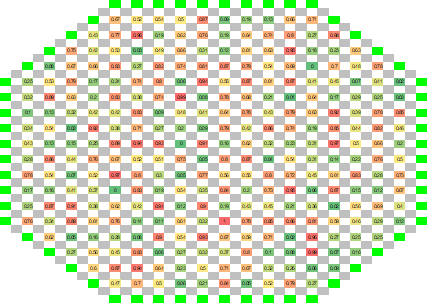
\includegraphics[scale=0.4]{Figures/agr_output.png}
	\caption{AGR Output Core Array}
	\label{fig:output_array}
\end{figure}

\noindent
A single iteration of the aforementioned process, summarised in Figure~\ref{fig:traditional}, gives us very little information on its own. With multiple iterations of this process, each with a different randomised state of the input array (Figure~\ref{fig:core_array}), a stochastic  understanding of the problem space can be built. For example, with several hundred iterations, a histogram can be plotted, as shown in Figure~\ref{fig:statistical_analysis}. The frequency of results is then fitted to a statistical distribution, such as the Normal distribution. Using this distribution, it can be determined what percentage of results are above an acceptable threshold (for instance, half the bore radius shown in \ref{fig:bore_clearance}). Using these statistics, determinations can be made of the probability of certain serious events occurring and are used in safety decision making.\\



\noindent
Both of these engineering modelling methods mentioned in this subsection are expensive in terms of time, computation and/or materials. This expense represents a significant bottleneck to the process summarised in Figure~\ref{fig:traditional}.\\

\noindent
There are also ongoing inspection results to determine the actual positions of cracks. During any inspection interval it is only possible to examine a small number of bricks for cracks. Further, the inspection schedule is infrequent (once every 1 - 3 years) and it is difficult to forecast where new cracks will occur. In the future, improved inspection techniques and better understanding of the process that leads to cracking will yield better information about where and when cracks will occur.

\begin{figure}[b!]
	\centering
	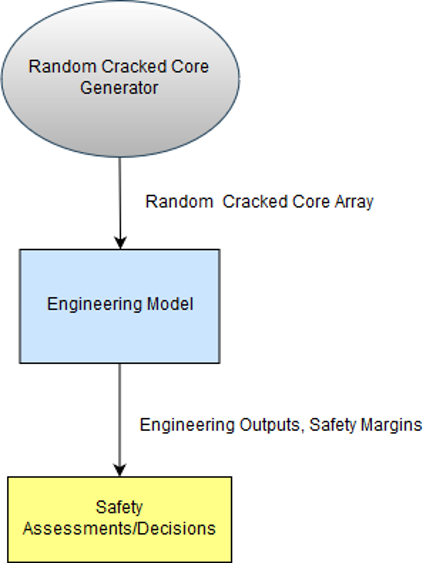
\includegraphics[scale=0.5]{Figures/engineering_approach}
	\caption{Traditional Engineering Approach}
	\label{fig:traditional}
\end{figure}

\begin{figure}[t]
	\centering
	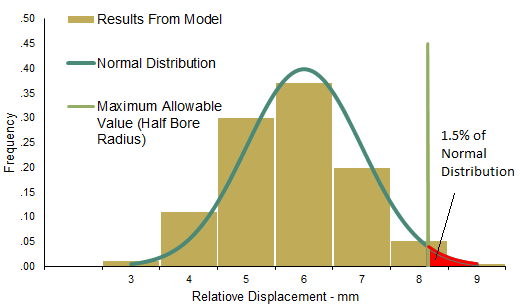
\includegraphics[scale=0.55]{Figures/Statistical_analysis}
	\caption{Statistical Analysis}
	\label{fig:statistical_analysis}
\end{figure}

\section{Relevant Literature}

The AGR reactor and its response to seismic activity is well studied in academic literature. In \cite{voyagaki2018earthquake}, both a computational and experimental examination of the AGR reactor is made. This paper discusses various seismic configurations, all involving an intact core i.e. without cracked bricks. The authors note that without cracking, an obstruction of a control rod channel during a seismic event is not possible due to the design of the core. Elsewhere, \cite{oddbjornsson2017physical} looks at the effects of cracking in a physical AGR experiment at the University of Bristol. The results of this work help validate computational studies. A noteworthy finding is that displacements tend to be greater near the centre of the core.
\chapter{Machine Learning Background}
\label{cha:ML}

This chapter gives an introduction and explanation of several machine learning techniques and the theory behind them. The areas to be explored include: supervised learning, neural networks, convolutional neural networks, surrogate machine learning models and transfer learning. 
\\

\noindent
For a more detailed explanation of the theory and workings of machine learning, see \cite{bishop2006pattern}.


\section{Supervised Learning} \label{supervised}

In the fields of engineering and science, models are frequently produced in order to simulate mathematical or natural phenomena. In these areas, accurate information regarding the phenomena they study. Such information allows the testing of scientific hypothesis and forecasting of future events. But what defines a model? \\

\noindent 
What is common to almost all models is the presence on input variables  and outputs . The model will use a set of input values (which we'll refer to as x) to calculate an outputs values (which we'll refer to as y) that are of interest to those using them. We can approach the development of such models from a hard computing angle: that is, we can hardcode relationships between inputs and outputs based on known relationships. \\

\noindent
Lets look at an example from the domain we are studying in this PhD thesis. In the  field of nuclear engineering, it is important to be able to calculate the power output of a nuclear reactor (which we'll measure in kilowatts) as a function of conditions within the core (\ref{hard_power}).

\begin{equation} \label{hard_power}
	Power(kW)  \rightarrow f\{x\}
\end{equation}

\noindent
In this example, an output value (power) is calculated as a function of input variables (x). There are of course a multitude of other factors that affect core power, however, the point of this example can be made with these four:


\begin{enumerate} [label=$x_1$]
	
	\item \textbf{Fuel Enrichment:} The useable content of the nuclear fuel at the time fuel is inserted into the core. Power level would increase linearly as enrichment rises. This value is measured as a percent of the total mass of the fuel and is usually between 1\% and 5\%.
	 

\end{enumerate}

\begin{enumerate} [label=$x_2$]
	
		\item \textbf{Time Since Refuelling:} The length of time since the core was refuelled. As this time increases, the power level would tend to drop as the useable content of the fuel is used up. This power fall would be linear at first, but the rate would accelerate  after a certain point due to the build up of fission poisons within the core. This value is measured in hours.

\end{enumerate}

\begin{enumerate} [label=$x_3$]
		
	\item  \textbf{Flowrate of Coolant:} The rate at which coolant is pumped into the core. This has a positive correlation with core power at lower rates, as the coolant (usually water) helps to sustain the nuclear chain reaction. However, this relationship breaks down after a certain flowrate, as certain concentrations of water act to block the fission sustaining neutrons. The flowrate would  is measured in $m^3$ per second.

\end{enumerate}

\begin{enumerate} [label=$x_4$]
	
	\item \textbf{Insertion Depth of Control Rods:} The control rods are inserted in order to slow or halt the nuclear chain reaction. Therefore, there is a negative correlation between insertion depth and power level. Lowering the power through control rod insertion has knock on effects, so the relationship is closer to the reciprocal of the square of the insertion depth. The unit is centimetres (cm). 
	
\end{enumerate}
\noindent
Using the relationships between these inputs at the output we wish to calculate, it would be possible to formulate a model to calculate reactor power output as a function of core configuration. However, from the complex relationships we discuss above, this would not be a trivial undertaking. The production of an effective model through hard computing techniques would require a strong understanding of the physical phenomena underpinning each factor. It would also be intensive in terms of effort from human domain experts. However, we may be able to formulate a model for this phenomena roughly in the form of (\ref{linear_model}). \\

\begin{equation} \label{linear_model}
	Power (kW) = f\{x_1\} + f\{x_2\} + f\{x_3\} + f\{x_4\} 
\end{equation}


\noindent
Alternatively, a model of this phenomena can be produced using soft computing techniques \cite{ibrahim2016overview} such as machine learning. Rather than hard coding relationships, a stochastic model is produced and optimised using a dataset containing examples of outputs and corresponding inputs. \\

\noindent
In machine learning terms, the output of the model discussed above can be calculated in the form of (\ref{soft_power}) .

\begin{equation} \label{soft_power}
	Power(kW)  \rightarrow f\{x, w, b\}
\end{equation}

\noindent
In this form, the output value of reactor power is calculated as a function of of our core configuration inputs (x) and a weight vector and a scalar bias factor. In machine learning practice, the input variables are referred to as features and the outputs are referred to as predictions. In our above example, there are four features (M = 4). \\

\noindent
The predictions of the model are generated on an instance by instance basis i.e. there is one predicted output per core configuration. The predicted output, which we will refer to as $\hat{y}$, is calculated for a for a given instance, i, in the form of (\ref{instance_prediction}).

\begin{equation} \label{instance_prediction}
	\hat{y}_i = x_i \space \cdot \space w + b
\end{equation}

\noindent 
In (\ref{instance_prediction}), the instance feature vector, defined as $x_i$, is simply the input values for the instance. The dot product between the instance feature vector and the weights vector, w, is calculated and then summed with the bias scalar.  For simplicity, we generally include the bias term when discussing the weights and to that end we shall define an extended weights vector which includes w and b (\ref{expanded_w}).

\begin{equation} \label{expanded_w}
	wb^T = [w_1, w_2 ... w_M, b]
\end{equation}

\noindent
At the start of machine learning model development, the expanded weights vector is initialised with random starting values. The values are then optimised through a model training process. To do this, we need a dataset including multiple instances of reactor power at various configurations of the core. For each instance in our dataset, there will be an input value for each of our features ($x_i$) as well as a corresponding output value that we refer to as the label (y). We refer to these input/output pairs as ground truth values - they are the base data that the model learns and evaluates its optimisation against.
\\

\noindent
The ultimate goal is to optimise the values of wb so that (\ref{instance_prediction}) can be used to make predictions ($\hat{y}_i$) that accurately reflect the ground truth labels ($y_i$). To make this optimisation, we must use a process known as gradient descent \cite{ruder2016overview} where values of wb are updated iteratively based on the derivative of difference between the predictions and ground truth. \\

\noindent
In order to perform the gradient descent operation and to evaluate the performance of our machine learning model, we require a loss function \cite{wang2022comprehensive}. This is a metric used to calculate the difference between the predictions of the model and the ground truth labels. Various ways exist to calculate the loss function, each having their own advantages and applications. Perhaps the simplest form the loss function can take is the mean absolute error \cite{willmott2005advantages}.\\

\begin{equation} \label{mae}
	\lambda_{mae} = \frac{1}{n}\sum_{i=1}^n | y_i - \hat{y_i} | 
\end{equation}

\noindent
Using (\ref{mae}), we can calculate a direct measure of the performance of the model against the ground truth, with the lower the value of $\lambda$, the better the model is performing.  We can also calculate the derivative of the loss function with regards to each element of the vector wb i.e. we can determine how much the loss function changes with a change in each weight. \\

\begin{equation} \label{derivative}
	{\Delta_{wb}}^T = [\frac{\delta\lambda}{\delta w_1}, \frac{\delta\lambda}{\delta w_2} ... \frac{\delta\lambda}{\delta w_M}, \frac{\delta\lambda}{\delta b}]
\end{equation}

\noindent
This derivative (\ref{derivative}) can be used to adjust the extended weights vector, wb, to a set of more more optimal values. This is done by multiplying the derivative, $\Delta_{wb}$, by the user defined scalar value $\alpha$, which is referred to as the learning rate. The values of this vector is then subtracted element-wise from the expanded weights vector to produce a new vector which can then be used again to make instance predictions as per (\ref{instance_prediction}). \\
 
 \begin{equation} \label{gradient_descent}
 	wb_{updated} = wb - (\alpha \cdot \Delta_{wb})
 \end{equation}
 
 \noindent
As can be seen from (\ref{mae}) the loss function (and its derivative) is an average over a set number of instances, n. Lets say the training process has access to a dataset of size N. We can perform the calculation from (\ref{gradient_descent})  using the entire dataset (n = N), a sample batch of the dataset (n $\subset N$), or a single instance (n = 1). If using a single instance or batch to update the weights (known as stochastic gradient descent \cite{ketkar2017stochastic}), the rest of the training set will be iteratively used to perform the same updating calculation. After updating using all instances in the dataset, it is unlikely that the expanded weights vector will be of the most optimal values.  Therefore, this process will be repeated a number of cycles known as epochs.

\begin{figure*}[h]
	\centering
	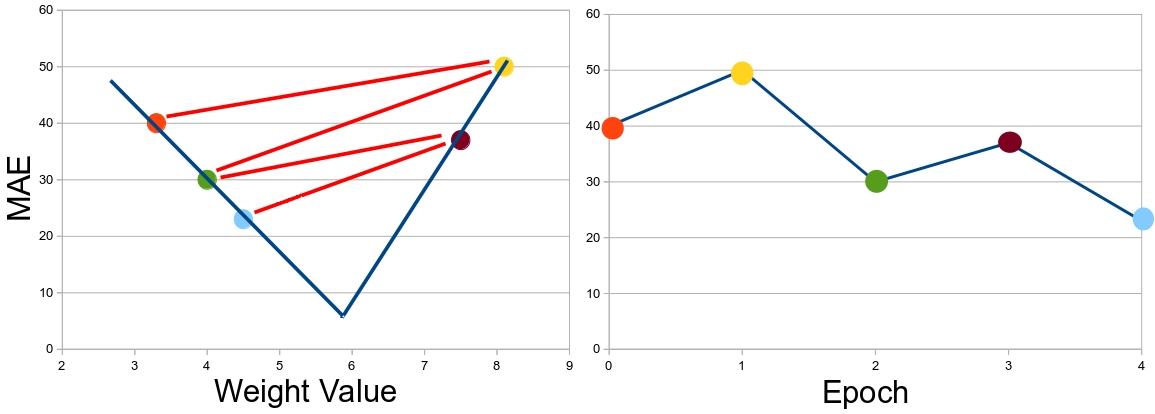
\includegraphics[scale=0.35]{Figures/gradientDescent_mae_bigLR.jpg}
	\caption{Machine Learning Model Training Process (Example 1)} {In this example, a machine learning model is trained over a period of four epochs. The mean absolute error (MAE) loss function is used as well as a relatively large learning rate which reduces each epoch (decay). \textbf{Left}: Loss history against the value of a single model weight.  \textbf{Right}: Loss history against epoch number.}
	\label{fig:GD_maeBigLR}
\end{figure*}

\noindent
In Figure~\ref{fig:GD_maeBigLR}, we see a representation of the training of a machine learning model. We see the progressive loss function calculated over a four epoch interval. This is expressed in two ways: (1) against the value of one of the model weights and (2) against the epoch number.  In this training example, gradient descent is performed using the MAE loss function and a relatively high loss function. This example also shows learning rate decay \cite{lewkowycz2021decay}, where the learning rate is reduced by 10\% successively after each epoch. \\

\noindent 
As mentioned previously, in most machine learning models, there will be multiple weights to optimise (one for each input feature). However, for this illustrative example, we will just focus on the optimisation of one weight.\\

\noindent
The chart on the left of Figure~\ref{fig:GD_maeBigLR} shows a theoretical topology of loss as a function of the example weight (dark blue lines at approximately 45 degrees from one another). At the start of training, we don't know the shape or nature of this topology, it is revealed through the training process. The target for any machine learning training operation is optimise all weight values to produce a model capable of achieving the lowest possible loss value - in the case of Figure~\ref{fig:GD_maeBigLR}, that is the hinge-point between the two dark blue lines. \\

\noindent 
In the aforementioned example, we can see that at the start of training (epoch 0), the weight is initialised at a value of around 3.2 which results in a MAE of about 40. From the gradient of the dark blue line at this point, it can be seen that increasing the weight of the value will tend to reduce the MAE. Feeding this negative gradient and the high learning rate into the subtractive term of (\ref{gradient_descent}) , we get an increased value of our example weight. As can be seen from the the loss time history, this operation actually results in an overshoot leading to a MAE that's actually higher than it was at the start of training (it now has a value of 50). This undesirable outcome is associated with a learning rate which is too high. \\

\noindent
For epoch 2, this time we are at a point in the loss-weight value topology where MAE is tending to increase as the weight value increases: a positive  . Recall that in this example, a learning rate decay is applied, meaning that the learning rate is 10\% lower than it was in the first epoch. This in turn means that the magnitude of the subtractive right-hand-side term of (\ref{gradient_descent}) is 10\% lower than it was in epoch 1. This reduction means that the updated weight is updated to a slightly higher point than the initialisation value. \\

\noindent
The following two epochs follow the same trend, however, the decaying loss rate means that progress towards the MAE minima slows. Further training would eventually see convergence with the weight and corresponding MAE value oscillating around a central value. At this point, further training is off little practical benefit. The practitioner may be able to manually apply early stopping \cite{yao2007early} or experimentally increase the number of epochs until this convergence point is reached. \\ 

\noindent
If we did not apply learning rate decay with the model training configuration of the aforementioned example , we may see a situation where a training process where the model fails to make any progress and repeatedly oscillates between the same two points. \\

\noindent
Lets now look at another example of gradient descent with alternative parameters. In our first example, we used the mean absolute error (MAE) loss function, now we will use instead the mean squared error (MSE) loss function (\ref{mse}). \\

\begin{equation} \label{mse}
	\lambda_{mse} = \frac{1}{n}\sum_{i=1}^n (y_i - \hat{y_i})^2
\end{equation}

\noindent
The mathematical difference between the MAE and MSE loss functions is that the inner term (the difference between the model prediction and ground truth label) is squared rather than simply the absolute. This alternative loss function has two practical differences in model training: 

\begin{enumerate}
	\item  Ground truth labels which are particularly large impact the loss calculation more severely. This can be beneficial when accurate prediction of outliers is of high importance.
	
	\item The loss-weight value topology is a curved U-shaped bend, rather than straight lines at a sharp angle (dark blue in the left of Figure~\ref{fig:GD_mseSmallLR}). This is because the derivative of this function with regards to the residual ($y_i - \hat{y_i}$) is variable rather than constant.
\end{enumerate}

\noindent
The other change is that we will assume a smaller initial learning rate than in the previous example.  In addition, we will not be decaying the learning rate. We begin with the same weight initialisation as the first example and loss starting point\footnote{In practice, the same residual ($y_i - \hat{y_i}$) would result is a different loss value for MAE and MSE (after all, they are different functions), but for these examples we assume equivalent values are calculated for each.}. \\

\begin{figure*}[h]
	\centering
	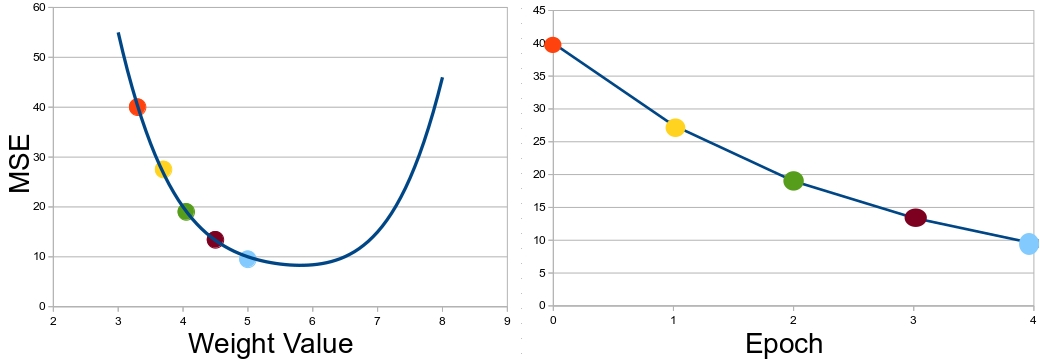
\includegraphics[scale=0.35]{Figures/gradientDescent_mse_smallLR.jpg}
	\caption{Machine Learning Model Training Process (Example 2)} {In this example, a machine learning model is trained over a period of four epochs. The mean squared error (MSE) loss function is used as well as a relatively small learning rate. \textbf{Left}: Loss history against the value of a single model weight.  \textbf{Right}: Loss history against epoch number.}
	\label{fig:GD_mseSmallLR}
\end{figure*}

\noindent
From Figure~\ref{fig:GD_mseSmallLR}, it can be seen that after one epoch of training, the weight value is updated only a small amount on account of the smaller learning rate. At this new point, the gradient of loss with regards to weight value is still negative, albeit to a smaller magnitude. On account of the subtractive term of (\ref{gradient_descent}) being smaller, the weight value update for the second epoch is somewhat smaller than the first. This trend can be seen to continue towards the base of the base of the curve. \\

\noindent
Comparing the performance of the two model training processes, it is possible to see the apparent advantages of the second configuration.  However, in practice different parameters have application in varying circumstances and conditions. The exact combination of parameters that are optimal for each problem must be determined through precedent (techniques found to be effective in previous works) and through experimentation.  \\

\noindent
In the previous examples, we saw the gradient descent method used to minimise loss towards the nadir of a loss topology. However, the topology for the full problem space might contain multiple minima regions. Figure~\ref{fig:minima_maxima} shows what such a topology with two minima regions: a local and global minima. If we wish to optimise the weights of our model, then we wish our gradient descent process to end within the global minima. However, depending on where our random initialisation of the weight begins, the convergence of our gradient descent process may end up in either region. \\

\begin{figure*}[h]
	\centering
	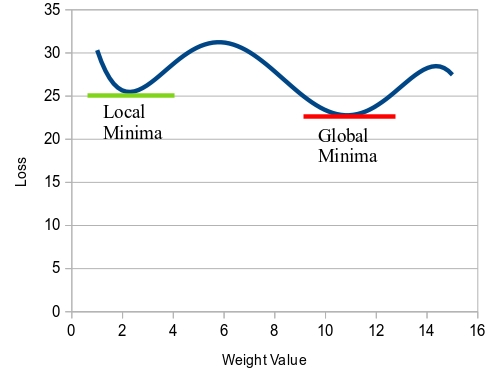
\includegraphics[scale=0.45]{Figures/loss_minima_maxima.jpg}
	\caption{Global Topology of Loss as a Function of Weight Value} {When looking at the full topology for the entire problem space, we see that there are there may be more than a single minima. }
	\label{fig:minima_maxima}
\end{figure*}

\noindent
How can we ensure that we obtain global optimisation and prevent the training process converging in a local minima? There are several techniques at our disposal:

\begin{enumerate}
    \item \textbf{Repeated Training}: If we are performing and experiment to evaluate a certain configuration of model parameters, it is prudent to repeat the training process several times. On each repeat, the weight initialisations will be randomised, giving a new starting points. By performing this experiment enough times, all of the global minima points should be achieved.
    
    \item \textbf{Learning Rate Schedules}: We saw in examples of gradient descent how a small learning rate can make our training process optimise closer to the nadir of a minima region. Similarly, a low learning rate can cause the training process to become trapped in a local minima. Having a large learning rate can allow the training process to cover a larger area of the loss-weight space and find a globally low region. We also saw earlier how learning rates can be changed during training, such as through decay \cite{you2019does}. To gain the benefits of both approaches, we can use a schedule of learning rates \cite{xu2019learning} to begin with a relatively high learning rate at the start of training, then have this fall when the model starts to converge of a minima region.
    
\end{enumerate}

\noindent
Once we have reached convergence with our gradient descent process, we may reach a point where our model is capable of making predictions very similar to the ground truth labels and hence produce a loss function calculation close to zero. We may be tempted at this point to think that the model exhibits a strong practical performance, but is this true? \\

\noindent
Consider that the dataset sample we use for training may represent only a small proportion of the entire problem space. It may in theory be possible to produce many thousands or millions of input feature/output label combinations than we have available for training. How can we be sure that our model is capable of making general predictions for the overall problem space and not just recalling training examples it has already seen? \\

\noindent
To answer this question, it is good machine learning practice to sequester a portion of our dataset at the start of the training process. We will call this portion the testing set and it will not be included as part of the data used to perform gradient descent i.e. the model will not have seen this data during training. Usually, we sequester around 70 or 80 percent of the dataset for training and retain the rest for testing \cite{gholamy201870}.\\

\noindent
At the end of training, we can evaluate our model against the testing set using our loss function. Hence, we are able to produce two loss calculations: a training loss and a testing loss. The earlier value gives a measure of the model's ability to fit to the training set, the later gives a more general measure of the ability of the model to actual make practical predictions for the problem space. \\

\noindent
A low or diverging training loss calculated during training suggests a model that is incapable of capturing the relationships within the training data. The training data may be invalid, or a value for a parameter such as the learning rate may have been inappropriately chosen (see the overshooting weight adjustment in Figure~\ref{fig:GD_maeBigLR}). A model which produces a low training loss and a high test loss is likely to have optimised too closely to the training set and has captured even irrelevant relationships between input features and output labels, such as noise or data errors. This model would be an example of one which is exhibiting overfitting \cite{ying2019overview} as shown in Figure~\ref{fig:overfitting}. \\

\begin{figure*}[h]
	\centering
	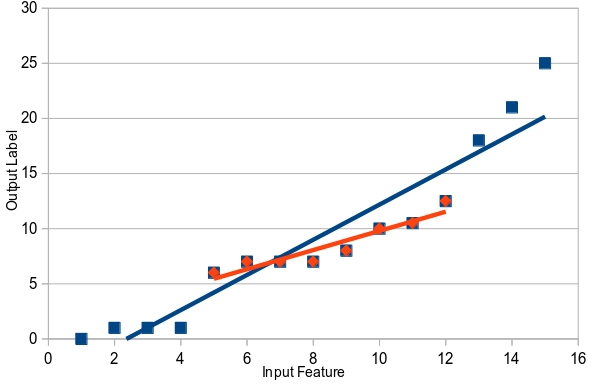
\includegraphics[scale=0.45]{Figures/overfitting.jpg}
	\caption{Example of a Linear Model Overfitting} {In this example, there are outliers at the lowest and highest points of the continuum.  It is possible that this data truly represents the underlying phenomena i.e. values at the lower end of the spectrum are indeed very low and values at the upper end are indeed very high. However, it is also possible that these outliers are due to recording inaccuracy and the true trend exhibited by the central data region (orange) should continue into the upper and lower regions. If this is the case then the linear model fit represented in dark blue is overfitting to the training data and may perform poorly on the testing set which may exclude these data inaccuracies. The linear model fit represented by the central orange line may be more representative of the true dataset trend.}
	\label{fig:overfitting}
\end{figure*}
		
\noindent
Another problem is that a machine learning model in this format can only model linear relationships between input features and outputs labels. Therefore, the gradient descent method described here may not be optimal for modelling the example scenario we discussed at the start of this section as there is a complex relationship between some inputs and the output value. For example, increasing the flowrate acts to increase and then decrease the power at different levels. This means that a linear model fit to this variable would incur inaccuracies as shown in Figure~\ref{fig:linearFit}. This is an example of underfitting \cite{koehrsen2018overfitting} where the complexity of a model is insufficient to capture the complexity of relationships within the data. \\		

% UNDERFITTING

\begin{figure*}[h]
	\centering
	\includegraphics[scale=0.45]{Figures/LinearFit.jpg}
	\caption{Example of a Linear Model Fitting to a Non-Linear Data Trend} {In this example a linear model of the type described in this section is fit to a non-linear data relationship}
	\label{fig:linearFit}
\end{figure*}

% TALK ABOUT DECISION TREES AND DO ANOTHE VERSION OF fig:linearFit with decison delineations
 
 \noindent
 To produce a machine learning model capable of accounting for these non-linear complexities, we must either look to neural networks, discussed in the next section, or to another type of machine learning model such as decision trees \cite{de2013decision} as shown in Figure~\ref{fig:DecisionTree}. This model has the added advantage of having a fully explainable decision making process that can be traced by a human observer. However, with added layers of branches for increased prediction resolution, the complexity of the model may no longer be easily comprehensible. Another advantage of decision trees is their ability to use categorical as well as continuous numerical inputs. An example would be branches representing high, medium and low rather than forks in a continuos values.
 
 \begin{figure*}[h]
 	\centering
 	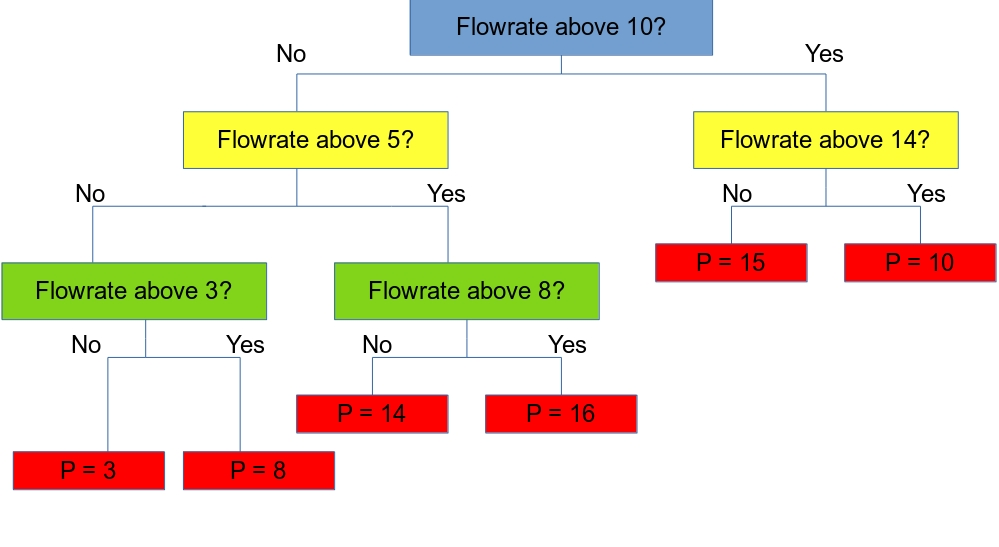
\includegraphics[scale=0.4]{Figures/DecisionTree.jpg}
 	\caption{Example of a Decision Tree} {}
 	\label{fig:DecisionTree}
 \end{figure*}


\section{Neural Networks} \label{NN}

The machine learning methods that we have explored so far in this chapter are commonly referred to as traditional or shallow methods.  The methods described in this chapter represent a stacking of machine learning operations in both parallel and series.  

\begin{figure*}[p]
	\centering
	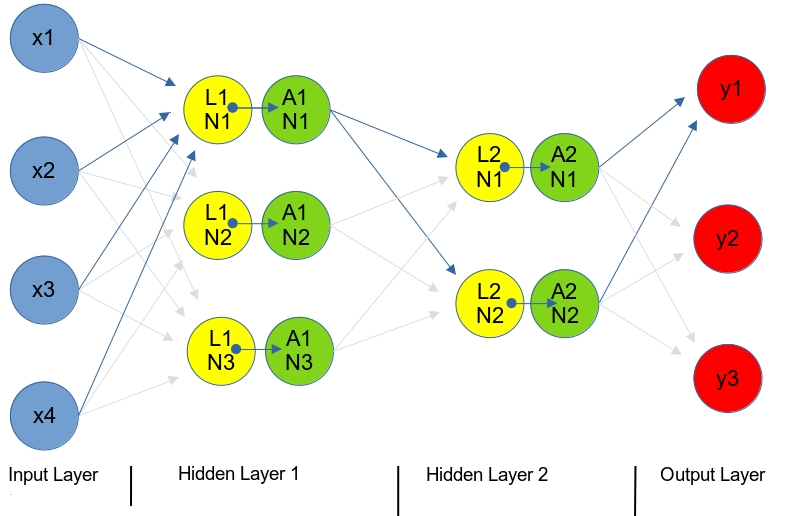
\includegraphics[scale=0.5]{Figures/NeuralNetwork.jpg}
	\caption{Neural Network Representation} {A neural network with an an input layer of four units, two hidden layers and an output layer of 3 units. At each yellow circle (node), a linear combination of the inputs leading to it is made. The calculated value is then fed into an activation function (green) which transforms it in a non linear way. The exception to this the output layer (red) where no activation function is applied.}
	\label{fig:neural}
\end{figure*}

\noindent
Figure~\ref{fig:neural} shows a representation of a neural network. A neural network has three main parts:

\begin{enumerate}
	
	\item \textbf{Input Layer}: Where inputs are fed into the network. This layer is akin to the model inputs described in section~\ref{supervised}.
	
	\item \textbf{Hidden Layer(s)}: This is where the neural network performs most of its calculations. This part may consist of a single layer or multiple. Each layer has one or more nodes, a point at which a linear calculation made similar to (\ref{instance_prediction}) is made in addition to the application of a non-linear activation function.
	
	\item \textbf{Output Layer}: This is the layer where outputs are fed out of the network. This is akin to the model outputs described in section~\ref{supervised} though there may be one or more output nodes i.e. the model may have more than a single model output. At each output node, the model makes a linear combination of the outputs from the previous layer, but does not apply an activation function as they do in the hidden layer(s).
	
\end{enumerate}

\noindent
The input layer from the example in Figure~\ref{fig:neural} has four inputs. These can be continuous numerical variables (as per traditional machine learning models) or representations of categorical data (an integer representing one of several categories).  For this example, they are the four model inputs discussed at the start of section~\ref{supervised} which are used to calculate reactor core power. However, we will modify x3 so as to be represented by a categorical value: 0 for low, 1 for medium, 2 for high flowrate. \

\noindent
For each dataset instance, the values from the input layer nodes are fed into each node in the first hidden layer. As each node performs the calculation shown in (\ref{instance_prediction}, each node also has as many unique weights as the number of nodes in the previous layer plus one bias term. \\

\noindent
As mentioned above, the output of each node in the hidden layers section of the network is normally passed through a non-linear activation function. The activation function can take one of several  forms and is a non trainable parameter - the user must select the activation function to be used by each node. The optimal configuration of activation functions used in the network can be determined through a process of experimental trial and error, through inspiration from previous machine learning works in the field, or some combination. \\

\noindent
Lets begin with an example starting at node L1N1 - i.e. \textbf{L}ayer 1, \textbf{N}ode 1. A linear combination of the four input features (x) is made with five trainable parameters equivalent to (\ref{instance_prediction}). The output of this calculation is then passed into adjunct node A1N1 (\textbf{A}ctivation 1, \textbf{N}ode 1) \footnote{The combined linear and activation function calculations are usually referred to as a single 'nodal' operation. However, for the sake of this example they shall we discussed as two operations.}. For this example, we will assume it to be the sigmoid function \cite{pratiwi2020sigmoid} that is applied. It is common to use the same activation function in all nodes within the same layer, and so we will assume A1N2 and A1N3 also uses the sigmoid function.\\

\noindent
Equation (\ref{sigmoid_activation}) shows the the sigmoid activation operation performed at A1N1 which is a function of the linear output of L1N1, $\hat{y}_{L1N1}$.  Figure~\ref{fig:sigmoid} shows the output of the sigmoid activation function. As can be seen, for strongly negative values of $\hat{y}$, the sigmoid function outputs values that tend towards zero. Between negative and positive four, the output value switches between zero and one, with the derivative of the function peaking around zero. \\ 

\begin{equation} \label{sigmoid_activation}
	\sigma_{A1N1} = \frac{1}{1 + \exp(-\hat{y}_{L1N1})}
\end{equation}

\begin{figure*}[p]
	\centering
	\includegraphics[scale=0.5]{Figures/Sigmoid.jpg}
	\caption{Sigmoid Activation Function} {A graphical representation of the output of (\ref{sigmoid_activation}) is given by the dark blue line. The derivative of this function is represented in light grey. As can be seen, the output rapidly switches between 0 and 1 between inputs of negative and positive four. This sigmoid activation function can be applied at activation nodes such as A1N1 in Figure~\ref{fig:neural}. }
	\label{fig:sigmoid}
\end{figure*}

\noindent
In this example and in most other activation functions, there is a notable threshold above which the output quickly switches between two values. In this example, the output is switching between 0 and 1 and can be thought of being equivalent to an electrical switch being on and off when a mathematical pattern is identified. \\


\noindent
Following the first hidden layer shown in Figure~\ref{fig:neural}, it can be seen that the activated outputs of A1N1, A1N2 and A1N3 are fed into each of nodes in hidden layer 2.  As they each receive three inputs, nodes L2N1 and L2N2 each have four unique trainable parameters (one weight for each of the nodes in the previous layer plus a bias term). Let us assume that A2N1, A2N2 use a softplus activation function \cite{zheng2015improving} which is similar to the rectified linear unit (relu) \cite{hara2015analysis}. \\

\begin{figure*}[p]
	\centering
	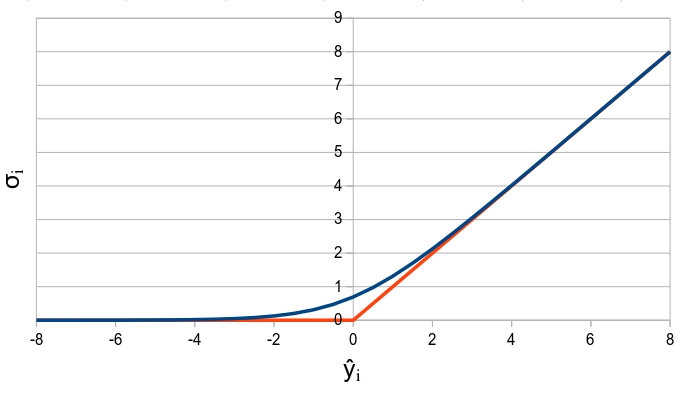
\includegraphics[scale=0.5]{Figures/softplus_relu.jpg}
	\caption{The Softplus and ReLu Activation Functions} { }
	\label{fig:soft_relu}
\end{figure*}

\noindent
Note that each of the activation functions represented in Figure~\ref{fig:soft_relu} contain a linear section and a threshold. This is in contrast to the symmetric sigmoid function we saw earlier and the hyperbolic tangent function \cite{anastassiou2011multivariate}. \\

\noindent
The final part of a neural network is the output layer, shown as red circles in Figure~\ref{fig:neural}. Each output node (y1 - y3) is a terminus for the aggregate nodal calculation performed throughout the network. Whereas the traditional machine learning methods described in section~\ref{supervised} can only generate a single output prediction, neural networks can generate multiple outputs.  In our example, these outputs might represent core temperature (y1)\footnote{Measured in degrees Kelvin}, core pressure (y2)\footnote{Measured in Pascals} and reactor power (as was predicted by the example models from the previous section). The ability to generate multiple predicted variables as part of a single machine learning model operation has advantages when users are likely to be interested in several variables at the same time. 
\\

\noindent
Each of the three red output nodes perform a linear combination of the outputs of the final hidden layer (A2N1 and A2N2) and its own unique weights and bias. Once again, each node in the output layer has one weight value for each node in the previous layer, plus a bias term. However, unlike hidden layer nodes, an output node representing a continuous variable isn't usually transformed by an activation function.
\\

\noindent
So far in this section, we have looked at how a neural network makes predictions by feeding inputs forward through several stages of nodal calculation. As we have discussed, each nodal operation involves several weights and a bias term. As they in the traditional methods discussed in section~\ref{supervised}, these weights and biases are initialised to a random variable at the start of training. In contrast to traditional methods, a neural network has a significantly greater number of trainable parameters. The training of these parameters again requires the use of gradient descent but using a more complex method known as backpropagation \cite{hecht1992theory}. \\

%\noindent
%Backpropagation again requires the use of a loss function that calculates a measure of difference between the predictions of the model and the ground truth labels. In this example we will again use the mean squared error (MSE) loss function as defined in (\ref{mse}), however, this time it must be adapted to calculate the loss for multiple model outputs. \\
%
%\begin{equation} \label{mse_multi}
%	\lambda_{multi\_mse} = \frac{1}{nk}\sum_{i=1}^n \sum_{k=1}^o (y_{ik} - \hat{y_{ik}})^2
%\end{equation}
%
%\noindent
%Equation~\ref{mse_multi} shows version of the MSE equation adapted for machine learning models with multiple outputs. The inner term calculates the square residual between output k of instance i. This is then calculated for all terms and summed over all n samples each having o number of model predictions in the output layer. \\  

%\noindent
%The gradient descent process is then performed at each node in the network. Like with traditional machine learning models, the trainable model parameters are updated by calculating the gradient of the loss function with regards to each weight and bias value. For the output layer nodes, the process  is similar to that for traditional methods as the prediction is the linear combination of the outputs from the previous layer and the weights \& bias term. For nodes in the hidden layers, an extra mathematical step is required due to the activation functions applied. \\
%
%\noindent
%Lets take the combined output of L1N1 \& A1N1 which was given by (\ref{sigmoid_activation}) , representing the sigmoid activation of the linear combination of model inputs and the weights \& bias term (\ref{L1N1}). \\
%
%  \begin{equation} \label{L1N1}
%  	\hat{y}_{L1N1} = x_1  w_1 + x_2 w_2 + x_3 w_3 + x_4 w_4 + b
%  \end{equation}
%
%\noindent
%The derivative of the sigmoid output (\ref{sigmoid_activation}) of node A1N1, $\sigma_{A1N1}$, with regards to weight $w_1$ of L1N1 is given by \\



\noindent
In the neural network arrangement we have discussed in this section, all nodes are connected to each other, hence it is often referred to as a dense or fully connected neural networks. We have seen one example of a neural network architecture in Figure~\ref{fig:neural}, but in practice this architecture could take a range of forms, with any number of hidden layers and nodes. The optimal arrangement can be determined by the user through experimentation, although there are a few common configurations which have proven effective for a range of problems. \\

\noindent
Apart from the ability of generate multiple outputs, a key advantage of neural networks over traditional machine learning models is their ability to model complex phenomena which may have non-linear relationships within the data. For example, in Figure~\ref{fig:linearFit} we saw the difficulty of fitting a predictive linear model to a variable which has a  non-monotonic relationship with the output variable. A fully connected neural network with an appropriately chosen architecture and choice of activation functions may be capable of modelling this relationship. \\ 

\noindent
As well as having advantages, 

% Large dataset needed
% overfitting
    % validation set monitoring 
    % Regularisation
    % dropout
% Exploding gradients
%vanishing gradients


\section{Convolutional Neural Networks (CNN)} \label{convolution}

\begin{figure*}[p]
	\centering
	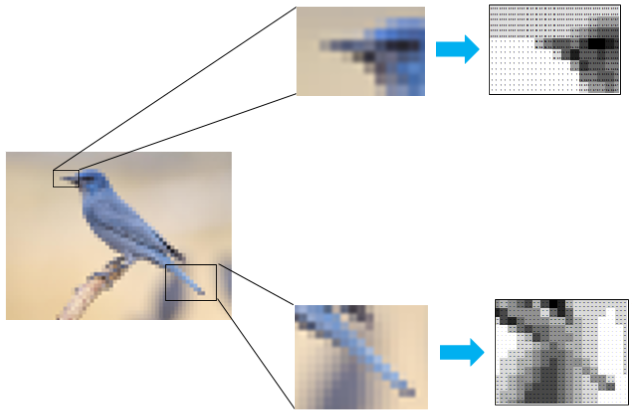
\includegraphics[scale=0.75]{Figures/cnn_feature.png}
	\caption{Convolutional Neural Network: Feature Extraction.}
	\label{fig:cnn_feature}
\end{figure*}

Convolutional neural networks (CNNs) attempt to capture local signals in data by use of a sliding window which passes over the input space. CNNs have been utilised in several areas of image analysis, including cell detection in medicine \cite{xie2015beyond} and depth estimation in photographs \cite{li2015depth}. Within the engineering field, they have been employed to predict remaining useful life of components \cite{babu2016deep}. The application of CNNs may be effective in the research problem discussed in this thesis as there are similarities between the data format for AGR graphite core analysis and image recognition, with the presence and identification of local arrangements important in both areas.
\\

\begin{figure*}[p]
	\centering
	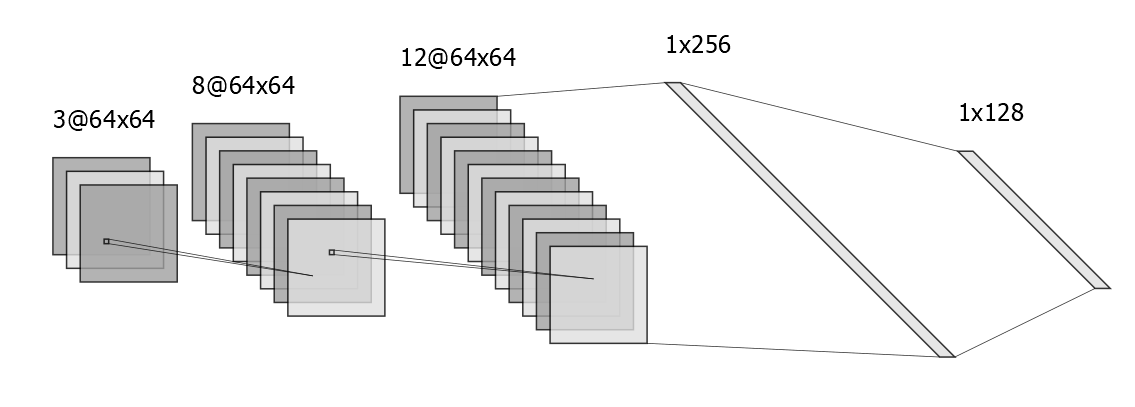
\includegraphics[scale=0.45]{Figures/cnn_arch.png}
	\caption{Convolutional Neural Network: Architecture.}
	\label{fig:cnn}
\end{figure*}

\section{Surrogate Machine Learning Models} \label{Surrogate}

For any given natural phenomena, it is possible to develop a physical model that mathematically describes it and can approximate its behaviour. Such phenomena range from a simple decaying wave (Figure~\ref{fig:surrogate}) to highly complex models such as that of turbulent fluid movement. Such models are unlikely to ever be a perfect representation of the natural phenomena, as there may be too many variables and factors to ever account for them all, hence there will always be some disparity. However, it may be possible to produce a model that is accurate enough so as to provide data that is of practical use.
\\

\noindent
From  data generated by such mathematical models, it is possible to train machine learning models to produce equivalent outputs from the same inputs. This will effectively be an additional layer of approximation on top of an already approximate model.
\\

\noindent
What is the motivation for doing this? Given a mathematical model of a phenomena, why develop and use a surrogate model using machine learning which provides inferior results? It is difficult to see why given the simple example of Figure~\ref{fig:surrogate}. However, in a real world case, such as nuclear reactor core safety, such a model may be highly complex, involving thousands of parameters and requiring significant computational expense. A machine learning model on the other hand, once trained, is computationally cheap to use, being just a series of matrix operations. The production of such a machine learning surrogate can also be seen as an exploration of the data space i.e. it is likely through the process of model training and refinement that insights into relationships between variables will be discovered. It may also be possible to develop machine learning tools so as to work in symbiosis with traditional mathematical models, with one informing the direction and focus of the other.
\\

\begin{figure*}[p]
	\centering
	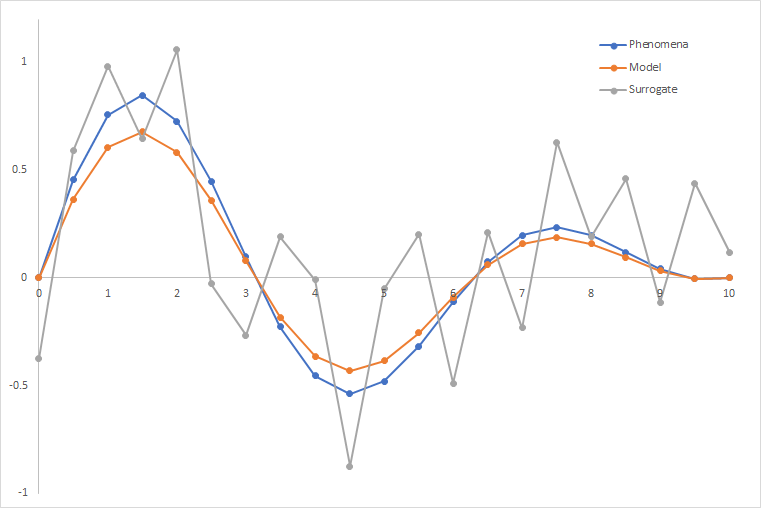
\includegraphics[scale=0.65]{Figures/surrogate_model.png}
	\caption{Modelling of Natural Phenomena} {A decaying wave (blue). A mathematical model may be developed which approximates its behaviour (orange). It may be possible to build a surrogate model (grey) which is an approximation built upon an approximation.}
	\label{fig:surrogate}
\end{figure*}

\begin{figure*}[h]
	\centering
	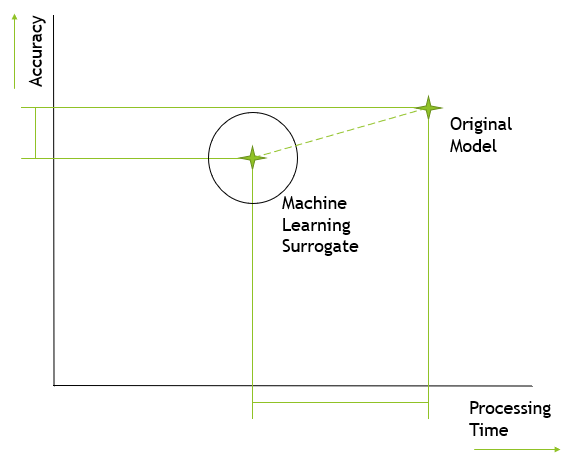
\includegraphics[scale=0.65]{Figures/MLS_vs_OM.png}
	\caption{The Trade-off Between a Machine Learning Surrogate Model and the Original Model} {Once trained on data from the original model, the production of new data is likely to be significantly more efficient in terms of computation and time. However, as the machine learning model is produced using data from the original model, there will be some inevitable reduction in accuracy.}
	\label{fig:surrogate_vs_model}
\end{figure*}

\noindent With each layer of approximation, there is of course an added margin of inaccuracy. Therefore, the development of a machine learning surrogate model is a trade-off between computational expense/time and accuracy (Figure~\ref{fig:surrogate_vs_model}).

\section{Transfer Learning and Existing ML Models} \label{transfer}

Many organisations have produced highly optimised neural networks, often demonstrating their capabilities in public competitions such as ImageNet \cite{russakovsky2015imagenet}. The successful competitors often publish their model architectures along with the best performing weights. Models produced and published through this competition include VGG \cite{simonyan2014very} and ResNet \cite{he2015deep}. Although these models are optimised to perform image classification tasks, many researchers have found that the aforementioned models can be adapted to other areas of study in a process known as transfer learning \cite{tan2018survey}.

\section{Relevant Literature}

An overview of machine learning techniques and their application to nuclear engineering is given in a recent paper \cite{gomez2020status}. This review details a range of machine learning approaches, including decision trees, nearest-neighbour, support vector machines, naive bayes, as well as Convolutional and recurrent neural networks. It then goes on to outline how these techniques have been applied in nuclear engineering fields such as plant health, radiation protection and optimisation. Although this paper does not reference the AGR or graphite, it does provide a useful introduction to the field. 
\\

\noindent
The same authors produced an earlier paper in which they use a neural network to predict the response of a light water reactor to various operational and accident conditions \cite{fernandez2017nuclear}. The motivations for this work include an ability to make rapid safety decisions (i.e. greater computational efficiency) as well as providing insight into safety issues. This research highlights various neural network architectures as shown in Figure~\ref{fig:architectures}.  
\\

\begin{figure*}[p]
	\centering
	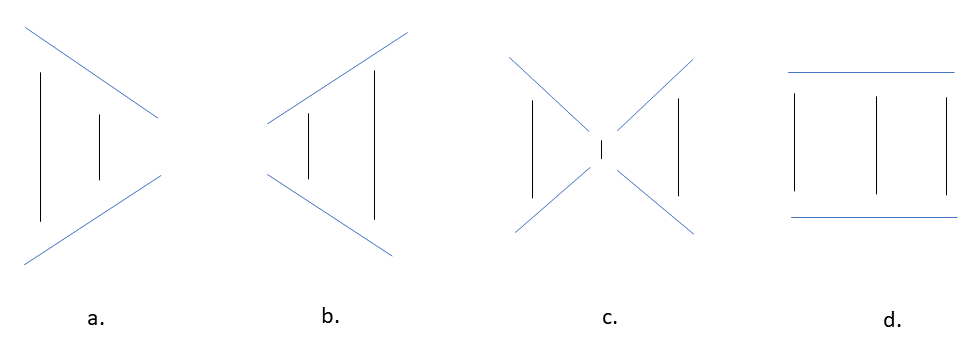
\includegraphics[scale=0.5]{Figures/architecture.png}
	\caption{Four Possible Neural Network Architectures} {Input on the left, output on the right. \textbf{(a)}: a narrowing structure where layers decrease in size towards the output layer and the output vector is smaller than the input vector; \textbf{(b)}: the inverse of a. with the layers increasing in size towards the output layer; \textbf{(c)}: An architecture combining both of the previous approaches, with the structure compressing the input and then expanding it before the output layer; \textbf{(d)}: A parallel structure where the layers remain of roughly similar size across the network. This Figure is a reproduction of Fig. 4 from \cite{fernandez2017nuclear}.}
	\label{fig:architectures}
\end{figure*}

\noindent
Academic works which apply machine learning to the production of engineering surrogates can be found as far back as 2003, where \cite{javadi2003neural} developed a symbiotic approach combine finite element models and neural network architecture. A more recent treatment of this topic can be found in \cite{kim2019machine} where the authors employ several approaches. These include an adaptive sampling method, where instances are generated and included in the training set based on their importance: i.e. selecting samples within the problem space that maximise useful information and excluding those which contain redundancy. Another relevant work is \cite{zeng2018machine} which uses a machine learning model to predict subsequent molten reactor core behaviour based on a time history. To train the ML model used in this work, the researchers generate data using a traditional engineering model (equivalent to that described in section \ref{Engineering}) to build a surrogate model (as described in section \ref{Surrogate}).  
\\

\noindent
A particularly relevant existing work to the PhD project discussed in this thesis is \cite{dihoru2018neural} which concerns both AGR graphite and machine learning. These researchers use data from a physical model of an AGR reactor which simulates an earthquake to train a feed-forward neural network (see Figure~\ref{fig:neural_network}) with 3 layers. The data generated by five configurations of the physical model (one intact, four with random distributions of cracks) are used to generate values for displacement in the top layer of the core. A neural network is then trained on this data, with displacements in the central channel being used to predict displacements in a select number of surrounding channels. The researchers achieve reasonably good agreement between model prediction and the ground truth data from their physical model, although there is some breakdown at the extremes. The scope of this model is somewhat limited, however, in that the model can only predict displacements from displacements at other locations. Superior model performance may also be achieved with a more complex neural network.  

\chapter{Dataset, Framework, Exploration and Analysis}
\label{cha:dataset}

This chapter has three purposes. Firstly, we explore  the data space using visualisation and statistical techniques. Next, we discuss the machine learning dataset generated using this data. Finally, we discuss the programmatic framework used to generate and manipulate the dataset.

\section{Dataset Exploration and Analysis} \label{data:visualisation}

To help choose a direction for research, a visual inspection of the dataset has been made. As mentioned in subsection~\ref{parmec:output}, the data produced by the Parmec model is multidimensional. Therefore, visual analysis will be made from multiple perspectives. The visualisations have been made possible through the framework that will detailed in the section~\ref{framework}. 

\subsection{Time History: Example Cases}


For a chosen Parmec case, Figures~\ref{fig:time_history_1} and \ref{fig:time_history_2} show the displacement time history for selected channels in two directions. It can be seen that the oscillations in displacement largely follow those of the earthquake acceleration pattern (Figure~\ref{fig:earthquake}). As expected, there is no displacement during the preliminary settle down period up to about 2.5 seconds. Channels near the centre of the core see higher amplitudes, with some of the most central channels also continuing to move after the earthquake has ended at around 8 seconds.  
\\

\noindent
Selecting four time frames from the earthquake time history, it is possible to visualise the displacement in the reactor core at these points. The time frames chosen can be seen in Figure~\ref{fig:earthquake} with vertical indicators and were chosen as they represent the peaks of earthquake acceleration. 
\\

\begin{figure*}[p]
	\centering
	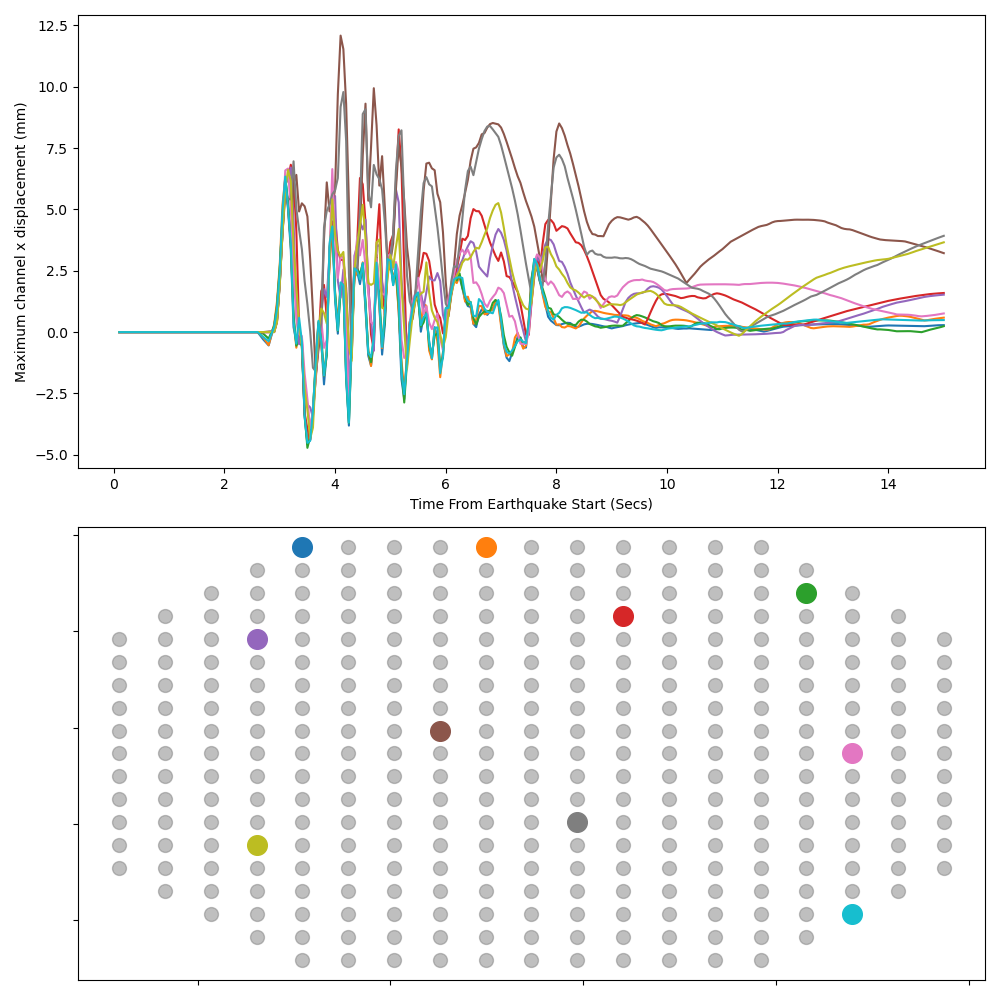
\includegraphics[scale=0.45]{Figures/time_history.png}
	\caption{Time History: Maximum Channel Displacement in the West to East Direction for Sample Channels} {Compare with the earthquake time history (Figure~\ref{fig:earthquake}).}
	\label{fig:time_history_1}
\end{figure*}

\begin{figure*}[p]
	\centering
	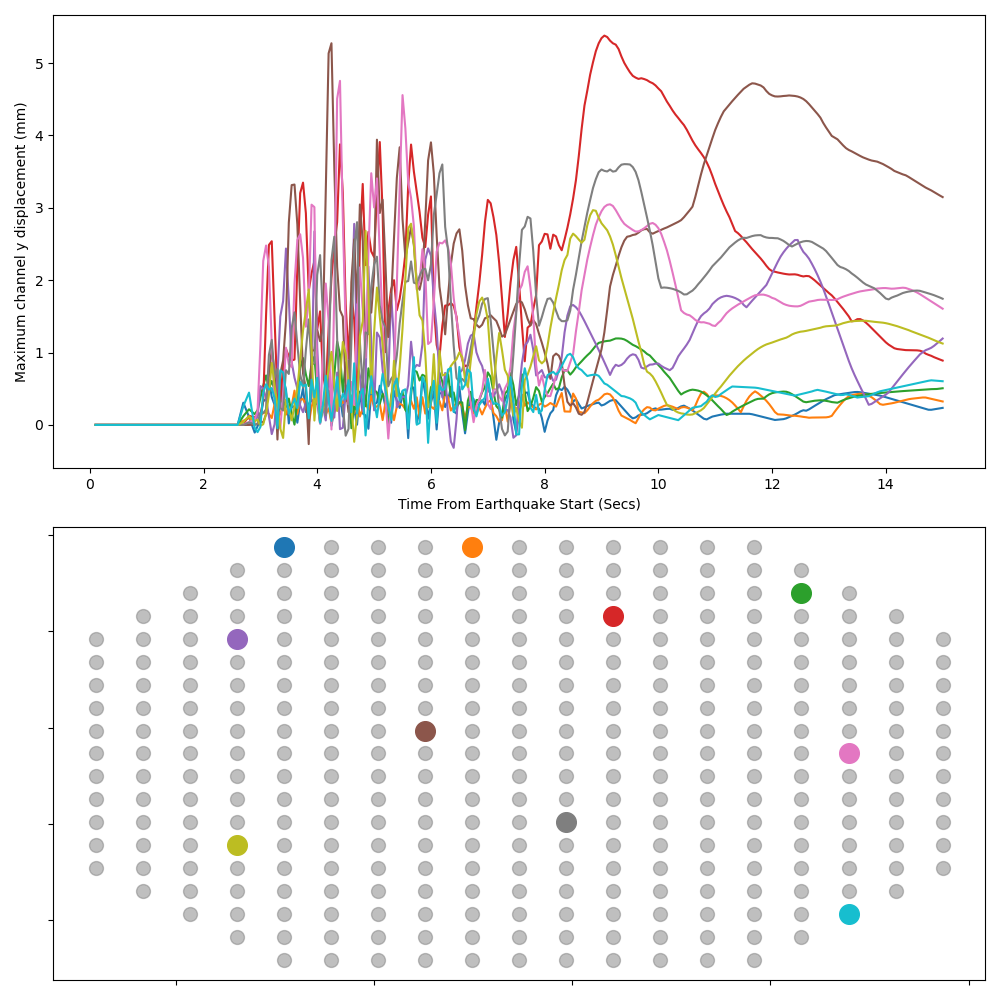
\includegraphics[scale=0.45]{Figures/time_history_y.png}
	\caption{Time History: Maximum Channel Displacement in the South to North Direction for Sample Channels } {Compare with the earthquake time history (Figure~\ref{fig:earthquake}).}
	\label{fig:time_history_2}
\end{figure*}

\noindent
A top down view of channel displacements can be seen in Figures~\ref{fig:results1}
and \ref{fig:results2}, where displacements in the west-east and south-north direction can be seen, respectively. For west-east displacement (Figure~\ref{fig:results1}), note that those channels near the edge of the core tend to displace in the opposite direction to those in the centre. For frames 65 and 68, there seems to be little diversity in the distribution of displacement values, whereas for frames 48 and 55 there is more variation, at least for the more central channels. For south-north displacements (Figure~\ref{fig:results2}) the displacements for each case are a variation on a similar pattern in each time frame.
\\

\begin{figure*}[p]
	\centering
	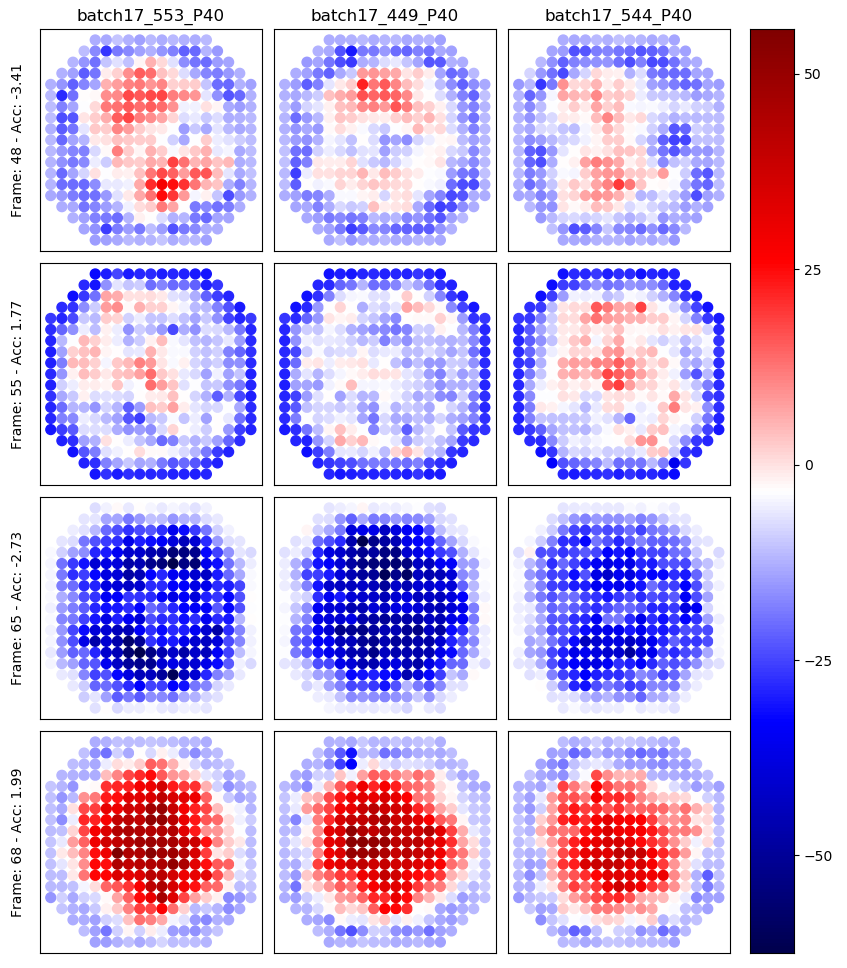
\includegraphics[scale=0.45]{Figures/results1.png}
	\caption{Comparing the Output of Three Cases Through Time: Sum of Channel Displacement in West-East Direction (mm) } { Three cases have been chosen at random from the dataset, corresponding to each of the three columns in this Figure. Each row corresponds to a time index of the earthquake (see the vertical markers in Figure~\ref{fig:earthquake}). The time frame is listed, as well as the earthquake acceleration at that time. The images are a graphical representation of the displacement value for each interstitial channel. Note that values are in the range $ \pm 50 $ i.e. the overall movement of that channel may be up to 50 mm in the left or right direction.}
	\label{fig:results1}
\end{figure*}

\begin{figure*}[p]
	\centering
	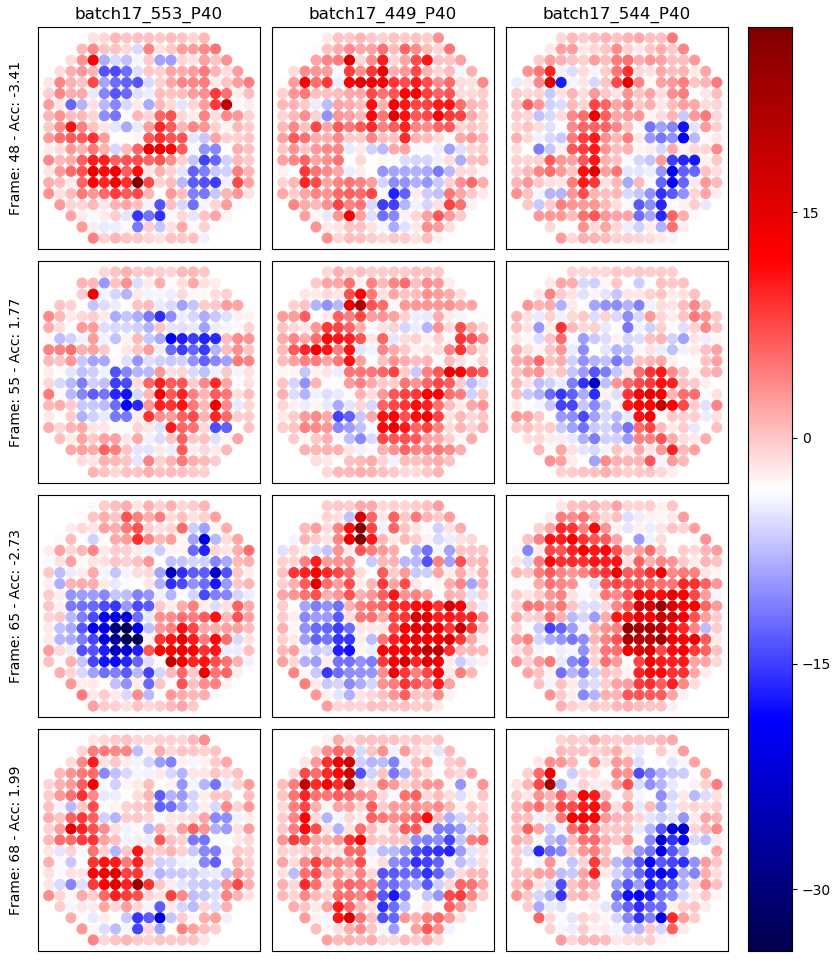
\includegraphics[scale=0.45]{Figures/results2.png}
	\caption{Comparing the Output of Three Cases Through Time: Sum of Channel Displacement in South-North Direction (mm) } {Three cases have been chosen at random from the dataset, corresponding to each of the three columns in this Figure. Each row corresponds to a time index of the earthquake (see the vertical markers in Figure~\ref{fig:earthquake}). The time frame is listed, as well as the earthquake acceleration at that time. The images are a graphical representation of the displacement value for each interstitial channel. Note that values are in the range $ \pm 30 $ i.e. the overall movement of that channel may be up to 30 mm in the south or north direction.}
	\label{fig:results2}
\end{figure*}

\noindent
For an alternative view on the previously illustrated example cases, the sum of level-by-level displacement can be seen in Figures~\ref{fig:levels1} and \ref{fig:levels2}. Similar to the top down view equivalent, Figure~\ref{fig:levels1} (west-east displacement) shows little variation across the three sample cases for frames 65 and 68, with slightly more variation on a similar pattern seen in frames 48 and 55. 
\\

\begin{figure*}[p]
	\centering
	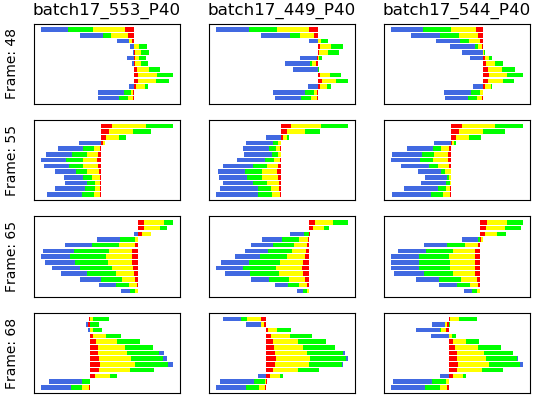
\includegraphics[scale=0.6]{Figures/level_results1.png}
	\caption{Comparing Output of Three Cases Through Time: Sum of Level Displacement in West-East Direction (mm) } {Three cases have been chosen at random from the dataset, corresponding to each of the three columns in this Figure. Each row corresponds to a time index of the earthquake (see the vertical markers in Figure~\ref{fig:earthquake}). The time frame is listed. The images are a graphical representation of the displacement value for each interstitial level.}
	\label{fig:levels1}
\end{figure*}

\begin{figure*}[p]
	\centering
	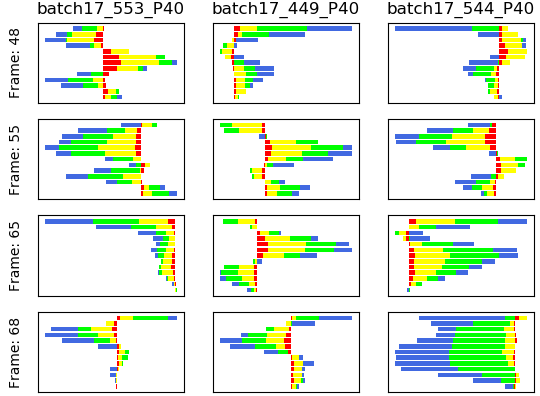
\includegraphics[scale=0.6]{Figures/level_results2.png}
	\caption{Comparing Output of Three Cases Through Time: Sum of Level Displacement in South-North Direction (mm) } { Three cases have been chosen at random from the dataset, corresponding to each of the three columns in this Figure. Each row corresponds to a time index of the earthquake (see the vertical markers in Figure~\ref{fig:earthquake}). The time frame is listed. The images are a graphical representation of the displacement value for each interstitial level.}
	\label{fig:levels2}
\end{figure*}


\subsection{Entire Dataset} \label{data:entire}


Several visualisations were generated based on the entire dataset of approximately 8300 samples. For the time frames highlighted in the previous section, Figures~\ref{fig:histo1} and \ref{fig:histo2} show histograms of all Parmec displacements outputs across all dataset samples. Note that for both displacement directions, the distribution of output values at each time frame fits around a central median value.
\\

\noindent
For a single time frame (48) Figure~\ref{fig:composite} shows a channel by channel summation of the Parmec results across the entire dataset. This allows us to make comparisons between core regions. The outer channels tend to have negative (eastward) displacement, indicated in blue. As we move closer to the centre of the core, the displacement moves towards zero, indicated in white. Moving further towards the centre of the core, the displacement becomes increasingly positive (westward), indicated in red. The displacement values have strong radial symmetry about the centre. The uniform structure of the Parmec outputs in the aforementioned figure are interesting when considering that the input crack patterns are randomly generated.  
\\


\begin{figure*}[p]
	\centering
	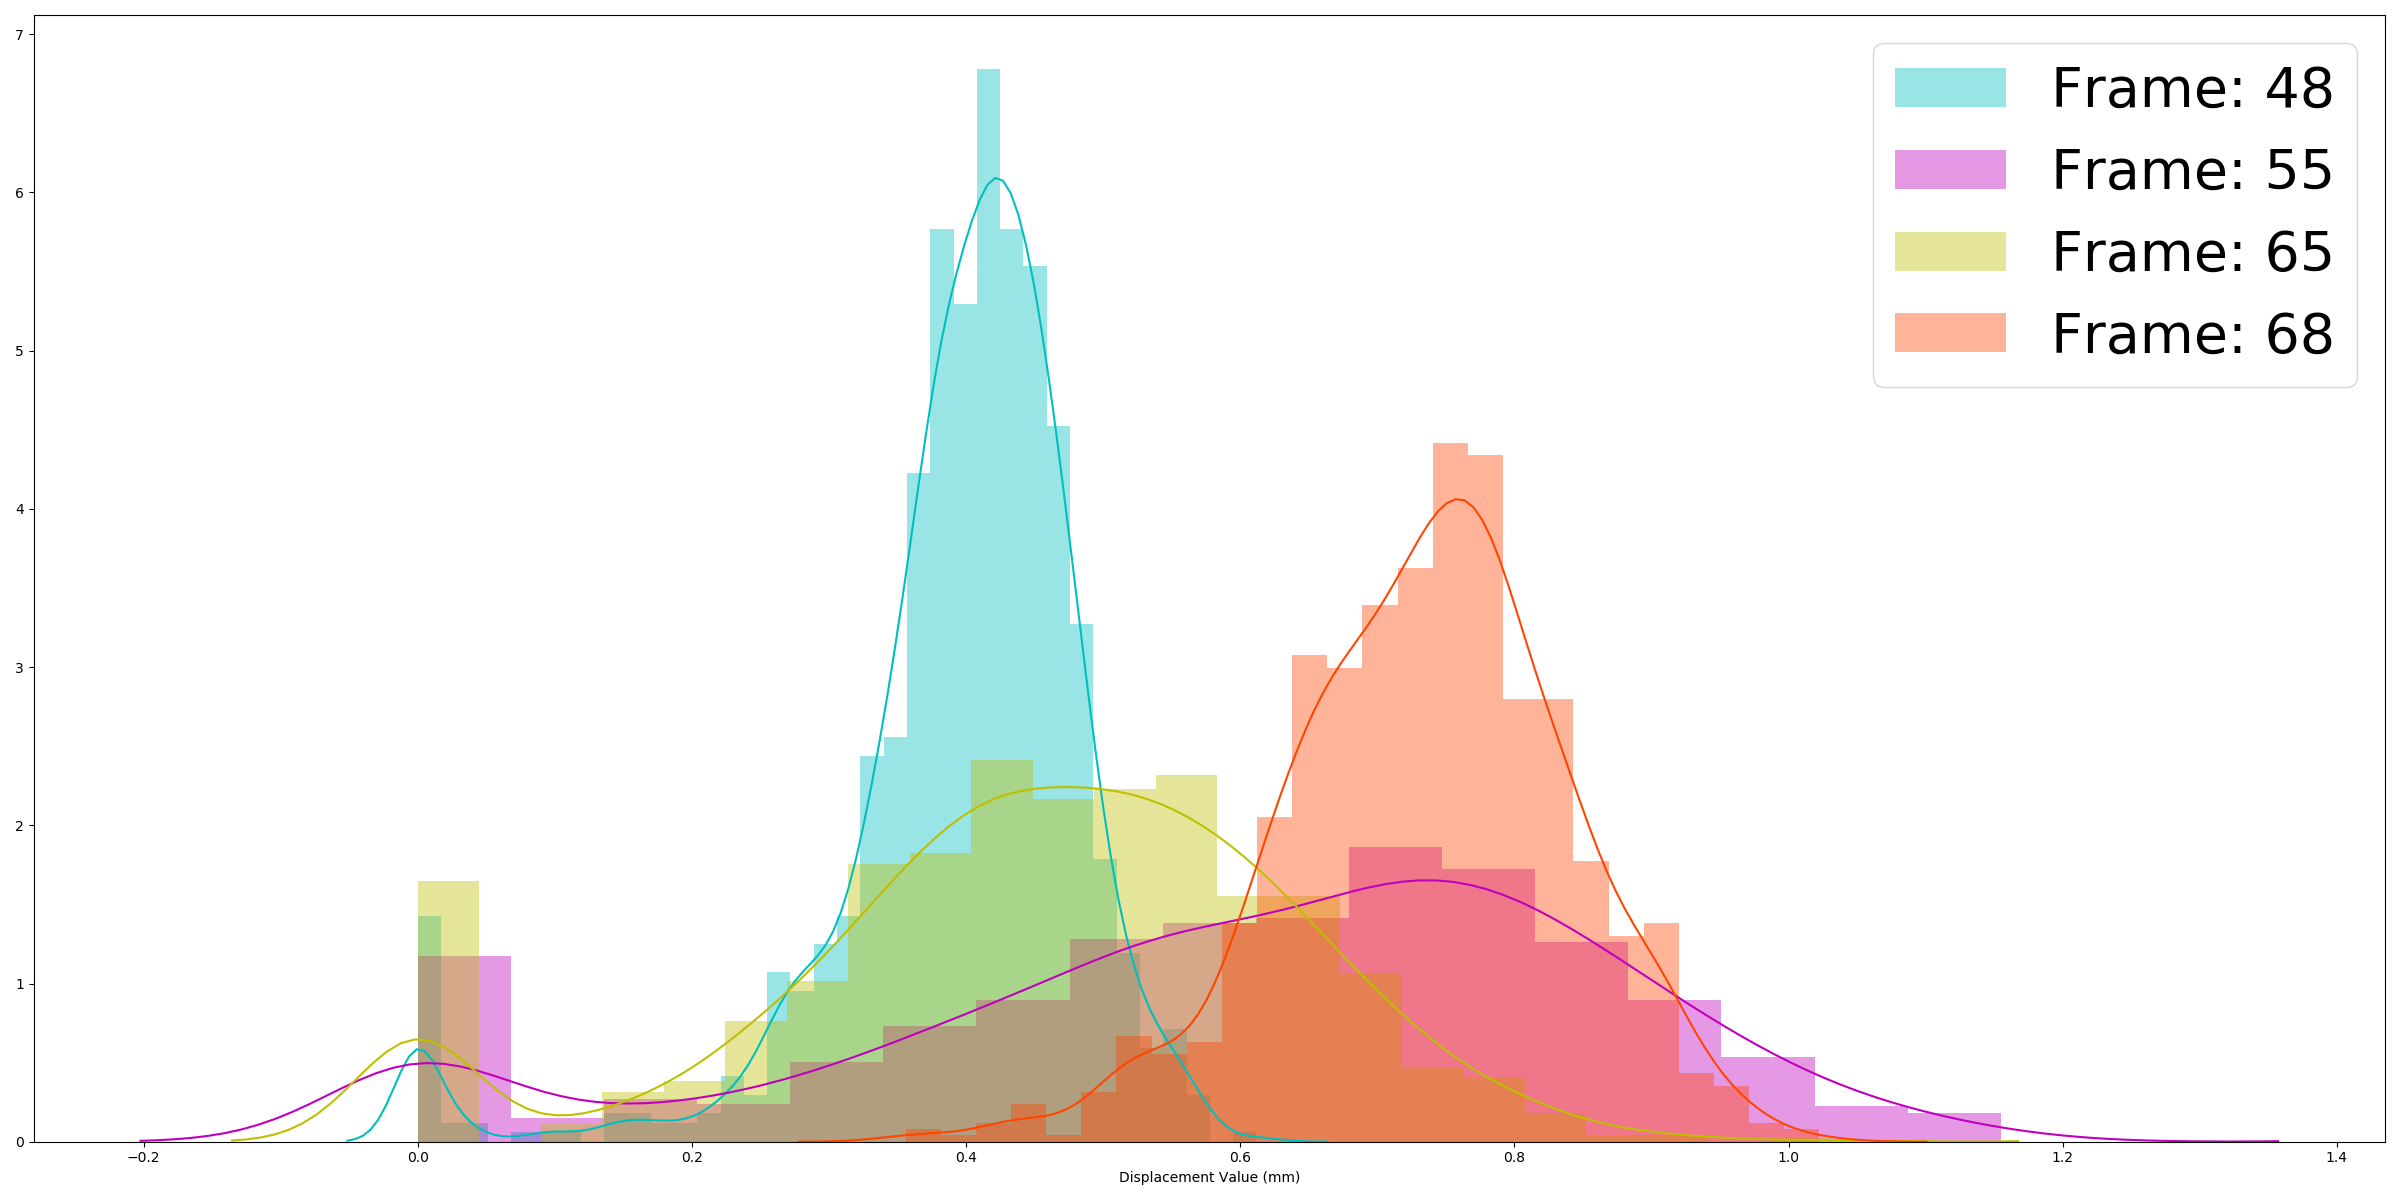
\includegraphics[scale=0.15]{Figures/histo1.png}
	\caption{Histogram of Sum Displacement of All Instances: West-East directional displacement } {This plot shows a histogram for results across the dataset. The results for each time frame are Gaussian in shape i.e. a symmetric bell curve around a mean value. However, there seems to be a smaller peak near the left tail.}
	\label{fig:histo1}
\end{figure*}

\begin{figure*}[p]
	\centering
	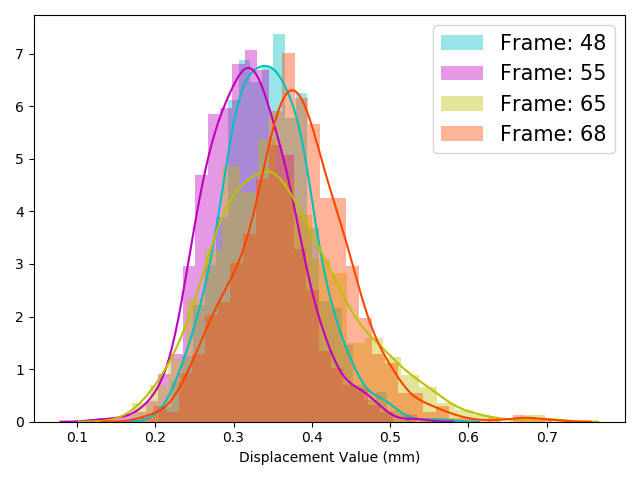
\includegraphics[scale=0.5]{Figures/histo2.png}
	\caption{Histogram of Sum Displacement of All Instances: South-North directional displacement } {This plot is very similar to Figure~\ref{fig:histo1}. A Gaussian distribution can be seen similarly to the previous plot.}
	\label{fig:histo2}
\end{figure*}

\begin{figure}[ht]
	\centering
	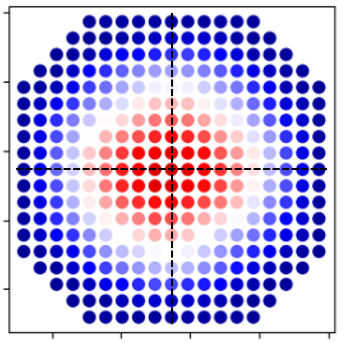
\includegraphics[scale=0.85]{Figures/compositeLines.png}
	\caption{Channel Summation for Time Frame 48 } {For each channel, the Parmec Outputs in the west-east direction were summed.}
	\label{fig:composite}
\end{figure}

\subsection{Output Correlation Analysis} \label{correlation}

\noindent A natural question at this point would be: how do the individual label values from \ref{instance_result_matrix} correlate with each other? For example, do the results for central channels increase when those for outer channels increase? Or is the opposite the case, or neither? \\

\noindent Consider again Figure~\ref{fig:inter_order} which numbers each of the interstitial channels. Note that channels are numbered in rows from left to right and hence numerically close channels are not always physically close - e.g. 75 and 76, which are on opposite ends of the core. Using the numbers from Figure~\ref{fig:inter_order}, consider Figure~\ref{fig:channel_correlations}. It appears that channels which are physically close correlate strongly, with this tendency breaking down the further a two channels are away from each other. This would suggest it may be difficult to train a model capable of making accurate predictions across the whole core.
\\

\begin{figure}[h]
	\centering
	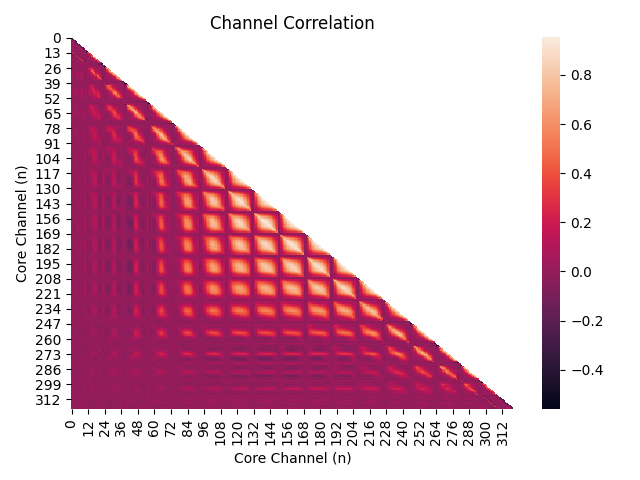
\includegraphics[scale=0.75]{Figures/channels_correlation.png}
	\caption{Correlation of Channel Results Against Each Other}
	\label{fig:channel_correlations}
\end{figure}

\begin{figure}[h]
	\centering
	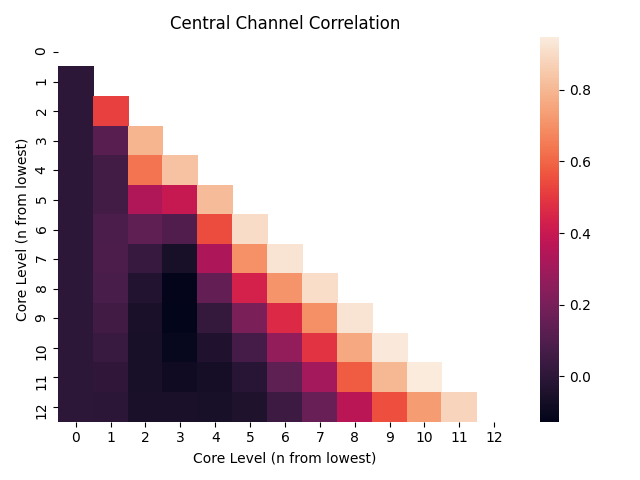
\includegraphics[scale=0.75]{Figures/central_channel_correlation.png}
	\caption{Correlation of Bricks of the Central Channel (161) Results Against Each Other}
	\label{fig:central_correlations}
\end{figure}


\noindent
Looking closely at only the correlations between results for the central interstitial channel (number 161 - see Figure~\ref{fig:inter_order}), we can again see a stronger correlation the closer two bricks are physically located (Figure~\ref{fig:central_correlations}).

\section{Machine Learning Dataset} \label{dataset}

8300 Parmec instances were generated to form the base dataset. Approximately 75\% of the dataset was randomly partitioned to become the training set (N) with around 6300 instances, with the remaining 25\% (2000 samples) forming the test set ($N_t$).  \\

\noindent
In subsection~\ref{parmec:data}, it was mentioned that the Parmec software can simulate  a core with cracked bricks representing anywhere between 0\%  (intact core) to 100\% (fully cracked) and that fuel bricks in the Parmec model can be modelled as having a single crack, or be double cracked. For the sake of this research, we shall choose a cracking percentage of 40\% and we shall model all cracked bricks as being double cracked. 

\subsection{Model Inputs (Features)} \label{data:inputs}



\begin{figure}[t]
	\centering
	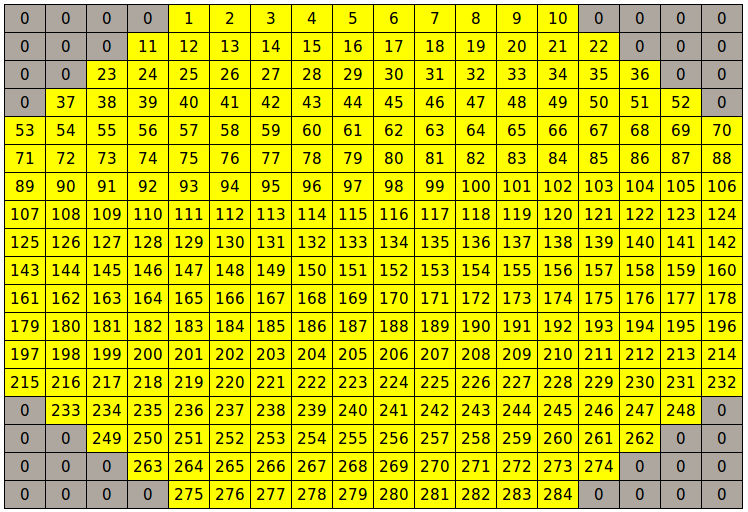
\includegraphics[scale=0.35]{Figures/fuel_channel_numbers.png}
	\caption{Fuel Brick Encoding Order}
	\label{fig:order}
\end{figure}


\noindent
The inputs for the Parmec model also serve as the input features to a machine learning model. The 3-dimensional input structure from Figure~\ref{fig:cascade} is unraveled into a 1-dimensional vector of length 1988. The cracking status of all fuel bricks are encoded according to their level (bottom to top) then by their position as shown in Figure~\ref{fig:order}. Note that at this point we are discarding the empty positions (zeros used to pad the corners). We are also discarding the orientation of the crack and only encoding a fuel brick as uncracked (-1) or cracked (1).
\\

\noindent
With 6300 training samples and 1988 input elements (cracked or uncracked AGR fuel bricks) this gives a matrix of dimensions N by BF (6300 x 1988), hence our feature matrix is defined as $\textbf{X} = \{-1, 1\}^{N \times BF}$. This matrix serves as the base input features to the machine learning models described in the following sections. 


\subsection{Model Outputs (Labels)} \label{data:outputs}

It is expected that part of the output tensor from Parmec (see subsection~\ref{parmec:output}) will become the output labels of surrogate machine learning model i.e. a SMLM will be developed to predict part of the Parmec output tensor. It is unlikely that a single SMLM will be able to accurately predict all of the ouputs from \ref{instance_result_matrix} due to its significant size. Therefore, we will have to narrow the output scope of the model, at least in the short term. We can do this in several ways: 1) We have already explored some research work published in the field of AGR seismic safety analysis (see section~\ref{engineering:literature}), 2) By making a visual and statistical analysis of the data (see section~\ref{data:visualisation})  and 3) through machine learning experimentation such as in section~\ref{prelim:whole}.


\section{Framework} \label{framework}

This section details the programmatic framework \cite{Jones2018} developed during this PhD. This framework was produced in order to streamline the development and optimisation of surrogate machine learning model for this project. The framework is provided free and open source with the intention that other researchers will adapt and use it for their own surrogate machine learning purposes. Using this repository, the accompanying dataset \cite{huw_rhys_jones_2022_6967536} and the attached guide, the method and results presented in this thesis can be reproduced by anyone.
\\

\noindent
The framework is developed so as to be useable on a portable batch system (PBS) as is commonly implemented on university cluster computing systems. These systems allow job queuing and parallel processing of experiments \cite{henderson1995job}. If a PBS system is not available, the framework is functional on any other standard computer.
\\

\noindent
The framework has six principal functions:

\begin{enumerate}
	\item The efficient and reproduceable creation of Parmec data 
	\item The extraction of relevant data from Parmec data cases
	\item The translation and engineering of the aforementioned data into datasets useable for machine learning training or testing 
	\item Machine Learning model design and parameter selection
	\item Model training \& evaluation
	\item Data visualisation and analysis including model performance 
\end{enumerate}

\subsection{Parmec Data Generation}

As mentioned in subsection~\ref{parmec:data}, the industry standard Parmec configuration file generator can only make single instances at a time and to non-reproduceable. As part of the machine learning framework developed for this PhD project, a Parmec case generation tool was developed which allows batch generation of instances, each traceable to a pseudo-random number seed \cite{blum1982simple}. This allows a creation of a large and reproducible dataset. Should the dataset be lost/corrupted or need to be temporarily deleted, it can be exactly reproduced using the original seeds.
\\

\noindent
The tool was developed by adapting an industry standard Microsoft Excel sheet with extensive changes using the Visual Basic .NET framework \cite{grundgeiger2018programming}. Using this tool, the user can batch generate Parmec configuration files by proving a comma seperated file of selected random numbers. 
\\

\subsection{Inputs and Outputs}

\noindent
For ease of use and interaction by the user, the framework converts each Parmec case into a data object, making use the object oriented programming (OOP) paradigm \cite{meyer1997object} with the Python language \cite{deitel2002python}. The Parmec class has interface methods which allow simple access and parsing of the information about that case. An additional layer of abstraction is provided by the creation of additional classes which aggregate all of the Parmec case objects in a batch of cases. This allows then generation of datasets for use in visual analysis or machine learning.
\\

\noindent
The Parmec case class allows the user to access input information about a particular case.  For example, should the user want to get the number of cracks in a particular level of the core. Used in aggregate across all cases within the dataset, the above input feature matrix as described in the previous paragraph can be efficiently obtained. 
\\



\noindent
The large amount of output data generated by Parmec is not in a format readily accessible or interpretable by human users or by other computer analysis. Therefore, the Parmec class object was extended to analyse this data and produce useable outputs. Again, this data is accessible via interactive Parmec object method calls and can be used in aggregate across the entire dataset.
\\

\subsection{Machine Learning Model Design}

The framework allows rapid design of the machine learning model architecture and the selection of parameters. This part of the framework is built upon the existing machine learning frameworks Keras \cite{ketkar2017introduction} and Scikit-learn \cite{pedregosa2011scikit} and also uses the matrix manipulation library Numpy \cite{harris2020array}. A machine learning model can be programmatically generated in a single line of code using the Model class from the framework, which contains arguments for number and types of layers, nodes, activation functions, loss function and learning rate.

\subsection{Machine Learning Model Training and Evaluation}

Once a dataset and base model have been obtained using the framework, it can then be used to train the model and evaluate it.  The model can be automatically retrained a set number of times from randomised starting weights in order to account for the stochastic nature of model training. \\

\noindent 
As part of a single experiment, a batch of differing model architectures or parameters can be selected and the performance of each compared. For instance, we could vary the number of layers of a particular type, then the framework will automatically generate, evaluate  and compare each one, allowing the user to select the optimal arrangement.  \\

\noindent
The framework aids the user in evaluating and comparing trained models through custom callbacks which execute and update the user throughout training using both numerical measures and visual representations of model performance. These include training \& validation loss histories, correlation plots of model prediction against ground truth values and prediction histograms. At the end of training, the framework presents the user with a summary of the experiment  including such values as minimum \& mean model loss, so that the user can make a high level judgement on the performance of parameter selections.


\chapter{Preliminary Machine Learning Experiments}
\label{cha:preliminary}

This chapter covers work which was completed as part of research for this PhD project, but were not included as part of a journal article. They include preliminary experiments, negative results and other exploratory research. 

\section{Dataset Size Sensitivity}

\noindent The motivation for this experiment was not to investigate the effectiveness of a particular method or approach, but rather to determine the sensitivity of model performance to data-set size. \\

\noindent From the larger data-set, 6000 cases  were randomly chosen. This set was split into 6 segments of equal size. The experimental procedure involved incrementally adding the segments to data-set used to train the model. After the adding of of each increment to the training data-set, the model was reinitialised with random starting weights so training could begin afresh. This process was repeated four times to account for the stochastic nature of the model initialisation process. \\

\noindent At each stage of the experiment, the data-set was randomly split into a training set (80\% of instances) and validation set (the remaining 20\%). The model architecture and parameters were kept constant for all increments of data-set size. The model used was a convolutional neural network, with 8 convolutional layers, each 64 nodes wide and 2 fully connected layers before the output layer. 
\\

\noindent 
Figure~\ref{fig:sensitivity_summary} gives a summary of the results for the experiment. Each pair represents a increment of the experiment, with the blue and orange bars representing the average training and validation loss at the end of the training process. As can be seen, the training loss after the final epoch is very similar in each increment. The average validation result, however, falls with each increase in the size of the data-set. \\

\noindent Looking more closely at the training process, we can examine the training loss history for each increment. Figure~\ref{fig:history_1000} shows that for a data-set size of 1000 instances, the training loss falls steadily, however, the validation rises steadily for the first 100 epochs and then converges. These seems to suggest the model is over-fitting with a data-set of this size. \\

\noindent When the data-set is increased in size to 3000 (Figure~\ref{fig:history_3000}), the training loss steadily decreases except for a spike at epoch 150. Similar behaviour can be seen for the validation loss, however, it appears to converge at around 200 epochs. Increasing the data-set size to 5000 (Figure~\ref{fig:history_5000}), validation loss convergence occurs at a lower loss value. Additionally, the training and validation losses at the end of training are closer to one another.
\\

\begin{figure}[b]
	\centering
	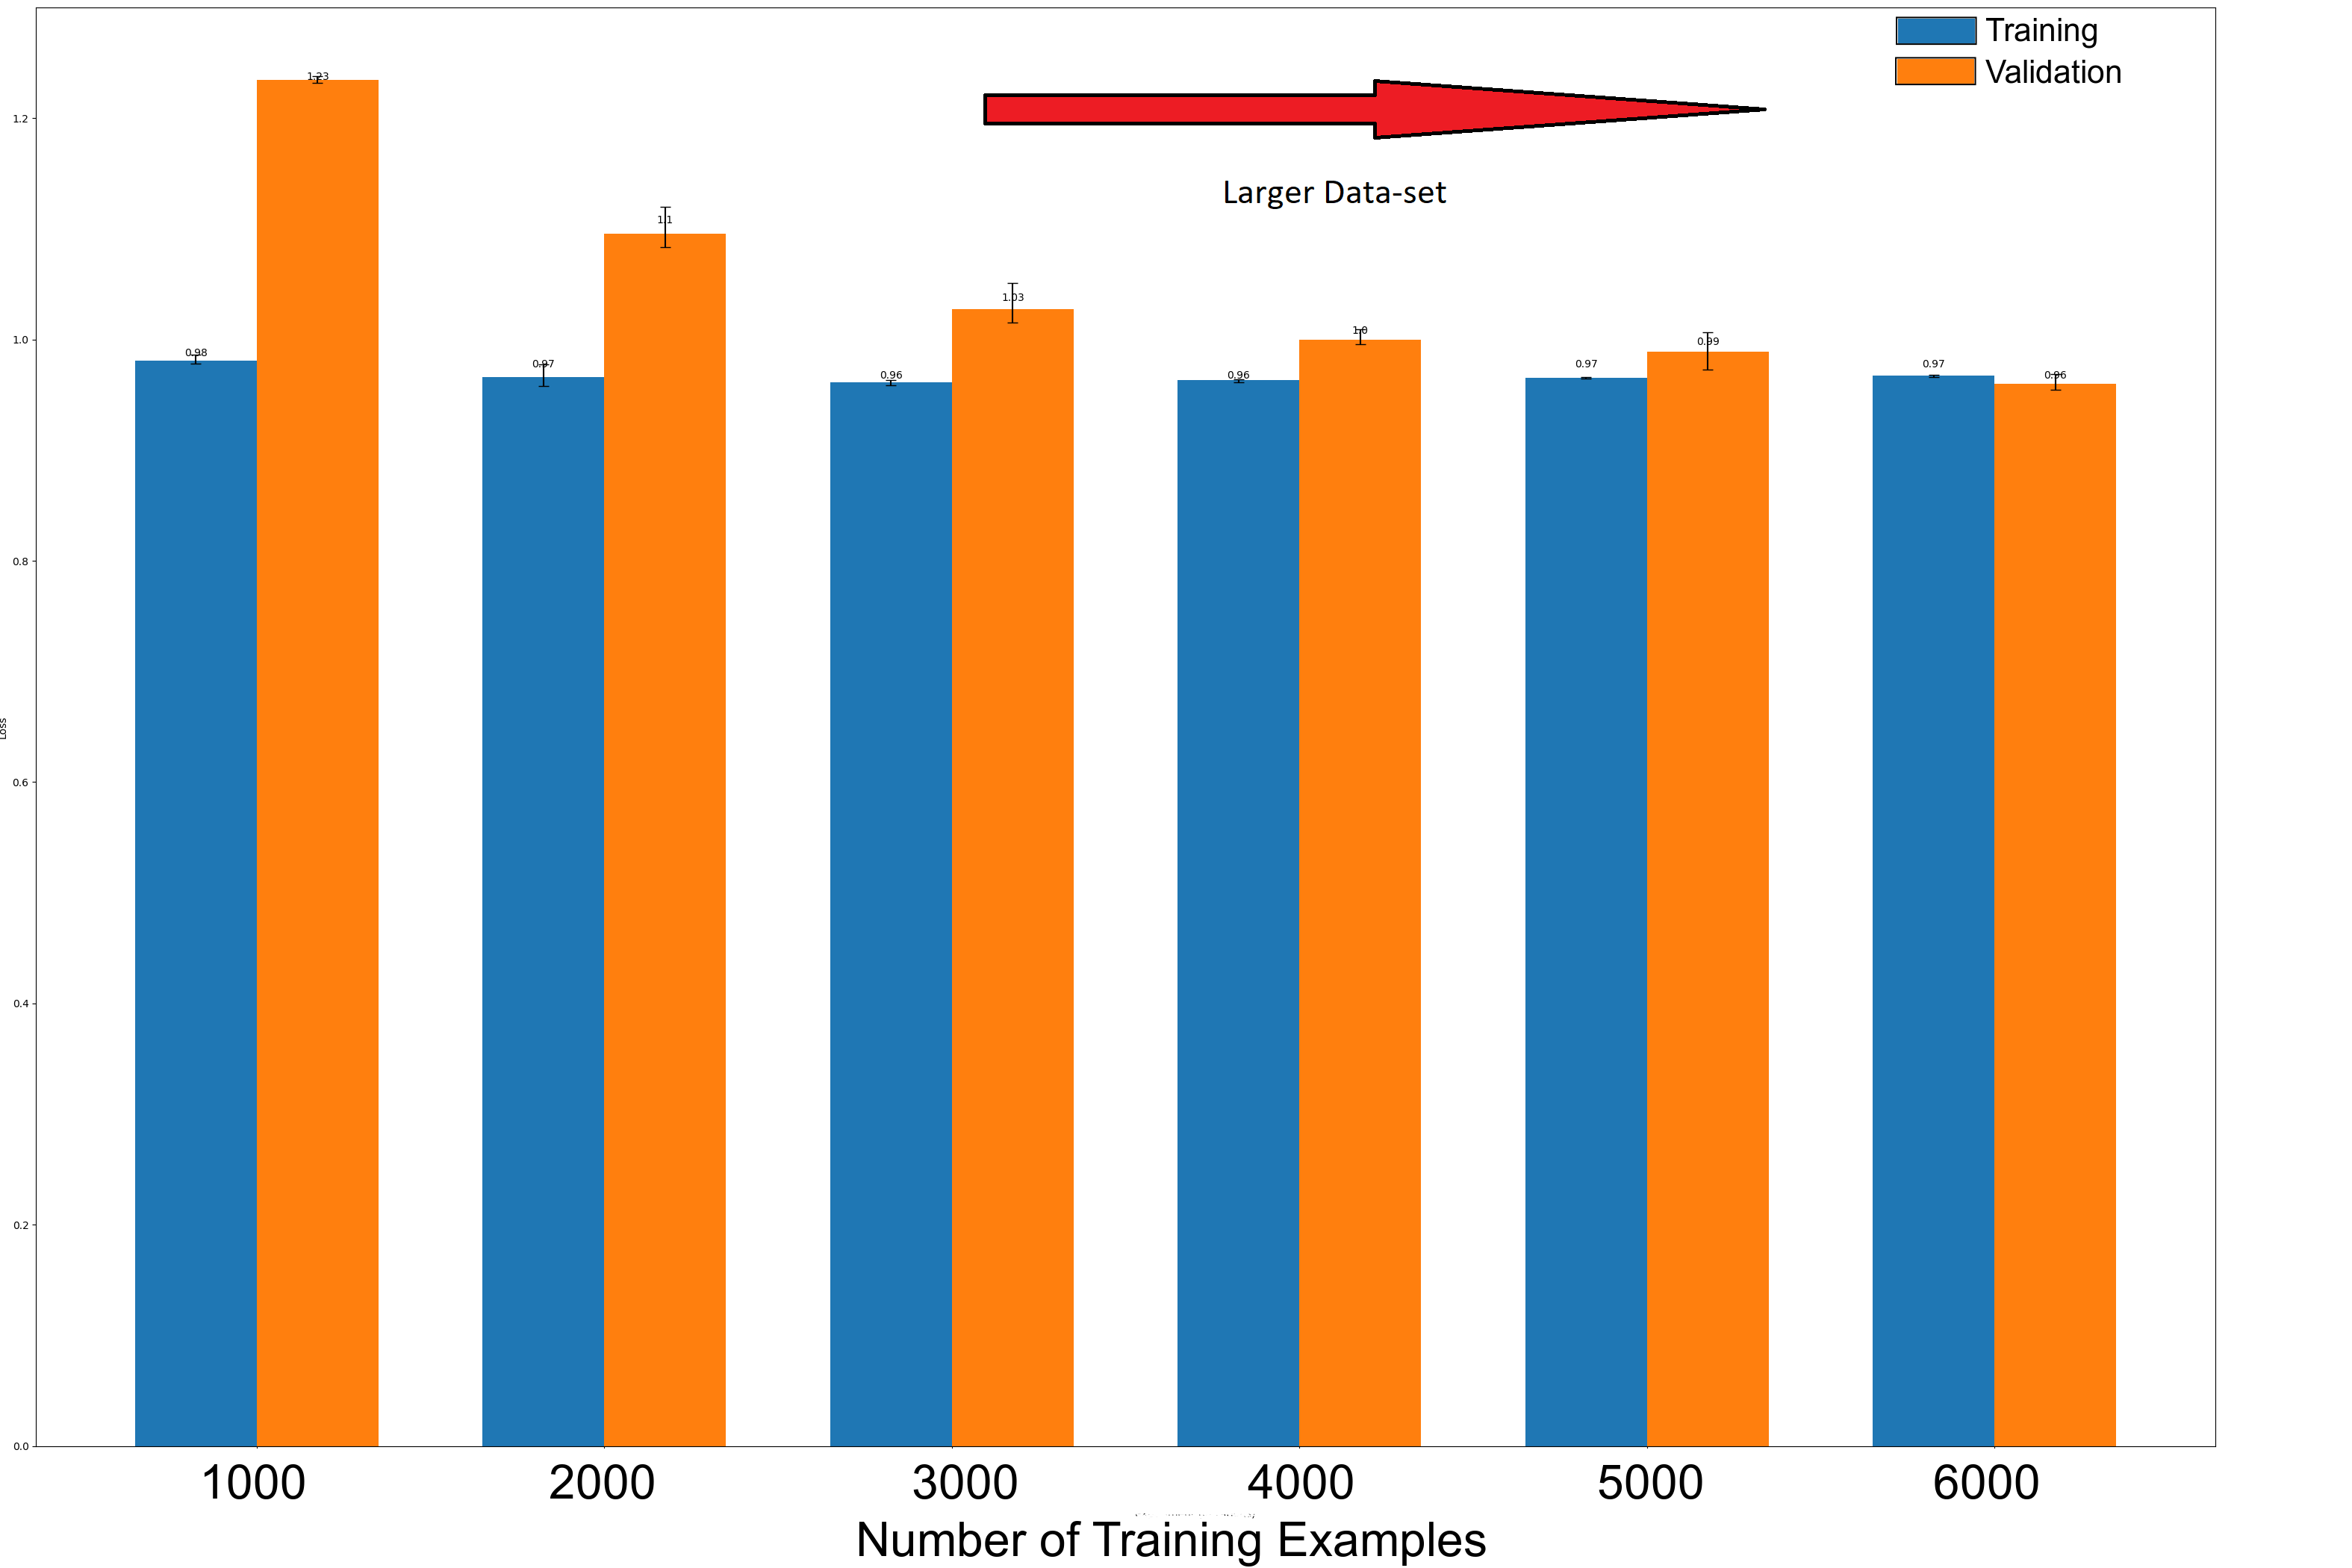
\includegraphics[scale=0.14]{Figures/comparing_models_Sensitivity.png}
	\caption{Sensitivity Results Summary}
	\label{fig:sensitivity_summary}
\end{figure}

\begin{figure}[b]
	\centering
	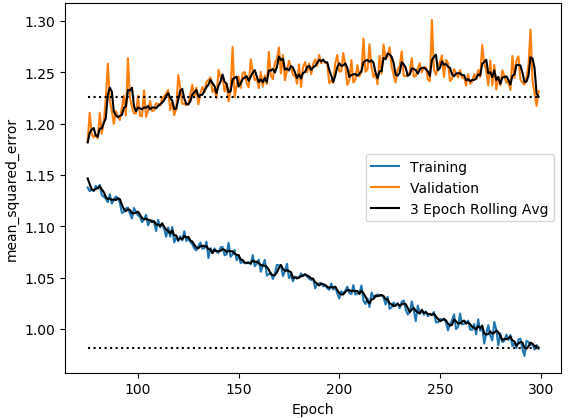
\includegraphics[scale=0.75]{Figures/TrainHistory_dataset_cases1000_C0_321_L0_13_0_321_0_13_48_1_allI0.png}
	\caption{Training History of Increment with a Data-set of 1000 Increments}
	\label{fig:history_1000}
\end{figure}

\begin{figure}[b]
	\centering
	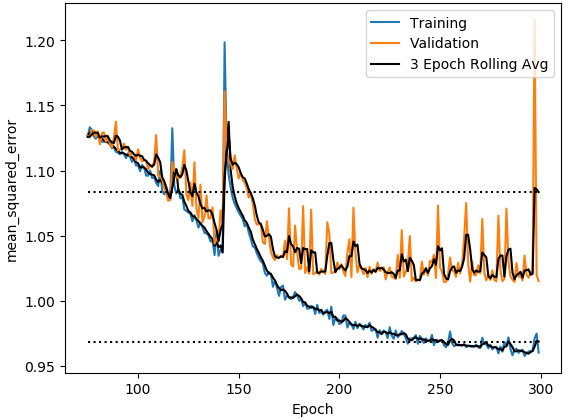
\includegraphics[scale=0.75]{Figures/TrainHistory_dataset_cases3000_C0_321_L0_13_0_321_0_13_48_1_allI0.png}
	\caption{Training History of Increment with a Data-set of 3000 Increments}
	\label{fig:history_3000}
\end{figure}

\begin{figure}[b]
	\centering
	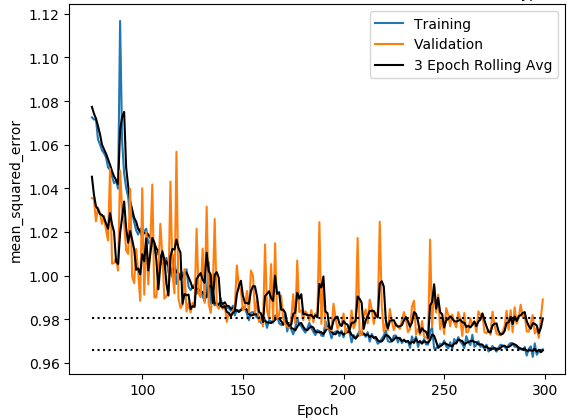
\includegraphics[scale=0.75]{Figures/TrainHistory_dataset_cases5000_C0_321_L0_13_0_321_0_13_48_1_allI0.png}
	\caption{Training History of Increment with a Data-set of 5000 Increments}
	\label{fig:history_5000}
\end{figure}

\noindent
It's clear from this experiment that a larger data set yields improved results. This result is as would be expected - a larger dataset yields more training examples for the model to learn from and reduces the potential for overfitting~\cite{hawkins2004problem}.  Looking carefully at Figure~\ref{fig:sensitivity_summary}, we can see performance improves sharply for the first two increments. Following this, we have diminishing returns, with the final two incremental increases in dataset size yielding only very small improvements in model performance.  This suggests that at 6000 samples,  the training dataset is reaching a point of saturation i.e. increasing the size of the dataset much further is unlikely to yield significant model performance. The results of this experiment implies that we should focus computational and research efforts into machine learning model refinement rather than generating more Parmec data. However, investigations of increasing the dataset by a significant amount, say by an order of magnitude, should be investigated at a later date. This may be possible through techniques such as data augmentation \cite{shorten2019survey}.


\section{Crack Orientation}

Recall from subsection~\ref{data:inputs} that our input feature matrix can be represented by $\textbf{X} = \{-1, 1\}^{N \times BF}$, with N being the number of training samples and BF being the number of fuel bricks in the Parmec model. Each element in this matrix is either a -1 (representing an uncracked brick), or a 1 representing a cracked brick. 
\\

\noindent
Note also that in subsection~\ref{data:inputs} it was discussed that Parmec can represent a cracked fuel brick in one of four orientations (see Figure~\ref{fig:orientations}). In the format of the input feature matrix discussed in the previous paragraph, the orientation of a cracked brick is not encoded and this information is discarded. 
\\

\noindent
If we wish to encode this information for the purposes of  developing a machine learning model, how we go about this? We could adapt our input feature matrix to the form $\textbf{X} = \{-1, 4\}^{N \times BF}$ so that a cracked brick is denoted by a 1 - 4 inclusive, representing one of the crack orientations shown in Figure~\ref{fig:orientations}. However, a machine learning model would treat these as ordinal values i.e. it would see orientation 2 as being double that of orientation 1. Effectively there is no ordinal relationship between the orientations and so this format would be incorrect.\\ 

\noindent
Instead, our feature matrix is expanded into an extra dimension. As opposed to a 0 or 1 for each brick representing an uncracked or cracked brick, each brick is now represented by a vector of length 4. An uncracked brick is represented by a vector of four zeros, with each crack orientation (Figure~\ref{fig:orientations}) represented by a 1 in one of the four vector elements (\ref{one_hot}).
\\

\begin{equation} \label{one_hot}
	\textbf{Uncracked} = \{0, 0, 0, 0\}  \notag
\end{equation}
\begin{gather}
	\textbf{Orientation 1} = \{1, 0, 0, 0\}  \notag
\end{gather}
\begin{align}
	\textbf{Orientation 2} = \{0, 1, 0, 0\} 
\end{align}
\begin{align}
	\textbf{Orientation 3} = \{0, 0, 1, 0\}  \notag
\end{align}
\begin{align}
	\textbf{Orientation 4} = \{0, 0, 0, 1\}  \notag
\end{align}

\noindent This approach is functionally similar to one-hot encoding \cite{seger2018investigation}, where categorical values are represented by a binary vector. \\

\noindent
In this experiment, two machine learning models were trained in parallel: the first using our original input feature encoding ($\textbf{X} = \{-1, 4\}^{N \times BF}$) and the second with our expanded input feature tensor which encodes cracked brick orientation \ref{one_hot}. In both parts of the experiment, the model architecture and all other parameters were kept constant.  The training and evaluation process was repeated four times per input encoding format, so as to account for the stochastic nature of hyper-parameter initialisation.
\\

\noindent It was expected that the model trained using the expanded input feature tensor would outperform  the model trained using binary encoding.  After all, it is the same experiment except for the additional information of crack orientations as well as positions. However, only a very similar performance was seen, or in some cases, slightly worse. It appears that the model training process exhibits overfitting - where the model too closely fits the training set, including any noise or irrelevant information.  A clear indicator of overfitting is decreasing training loss whilst validation loss increases i.e. the model fits to the training set so well that it losses the ability to generalise to data outside of it. Looking at the training time history of the model trained using crack orientations, this phenomenon can be clearly seen in (Figure~\ref{fig:history_ori}). It can be seen that the training loss falls monotonically, with the validation loss rising steadily i.e. the model's ability to generalise is falling. \\

\noindent There are several explanations for the unexpectedly lower performance of the model trained with the input features including orientations. The first possibility is that the positions of the cracks is the overriding factor of importance in terms of causing displacements, with the orientations having little physical effect. The other possibility is that the results are an artefact of the way they have been encoded or expressed to the model. Further study should be made to investigate this at a later time.

\begin{figure}[!ht]
	\centering
	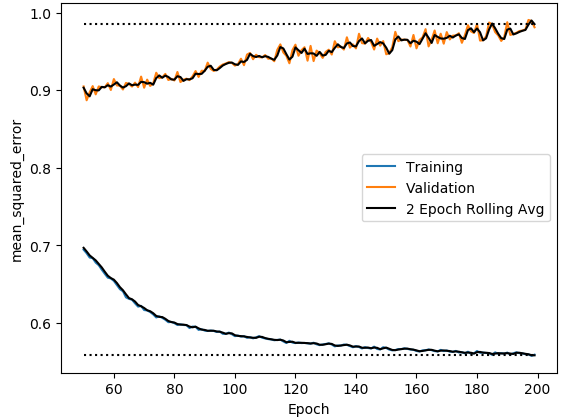
\includegraphics[scale=0.7]{Figures/train_history_ori.png}
	\caption{Training History for Crack Orientation Model }
	\label{fig:history_ori}
\end{figure}

\section{Transfer Learning}


As outlined in subsection~\ref{transfer}, existing models for image classification can be adapted to other problems, including the regression problem of this research work. Models from the VGG and ResNet families were adapted, including VGG16 \& VGG19 and ResNet50 \& ResNet101. These were trained and tested using the standard data-sets used previously. It was found that VGG19 performed the best out of all of these methods, with VGG16 also performing better than all ResNet models.
\\

\noindent
To suit the purpose of this study, the existing models had to be adapted. Previously, these models would receive a image tensor, usually of dimensions 32x32x3 (32 pixels width and depth plus 3 colour channels) and output a vector of length 1000 (representing a range of image categories). In place of the image tensor, the 3-dimensional tensor represented by Figure~\ref{fig:cascade} was flattened into a planar arrangement with an example shown in Figure~\ref{fig:transfer_encoding}. This was then one-hot encoded into three channels: cracked bricks (green), uncracked bricks (red) and corners/edges (blue). For each instance, this processes creates a input feature tensor of 88x44x3. The model output layer was modified to produce a single regression value.  
\\

\begin{figure}[h]
	\centering
	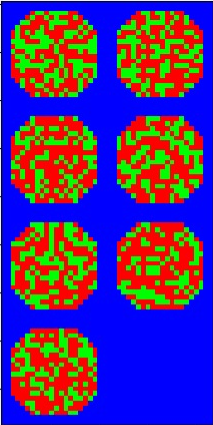
\includegraphics[scale=0.75]{Figures/vgg_encoding.png}
	\caption{Feature encoding appropriate for use in transfer learning} {This image shows a single Parmec instance encoded in a planar configuration.}
	\label{fig:transfer_encoding}
\end{figure}

\noindent
This experiment also involved adding layers between the end of the nominal VGG19 architecture and the output layer. These included dropout layers of varying percentages, dense layers of varying width and batch normalisation layers [\cite{liao2016importance}]. The summary of results can be seen in Table~\ref{tab:exp3}. It can be seen that simply adding a dropout layer of 30\% results in the best model performance uplift, with some adding reducing performance. A visualisation of the model performance can be seen in Figure~\ref{fig:results_transfer}. 

\begin{table}[h!]
	\begin{center}
		
		\begin{tabular}{c|c|c|c} % <-- Alignments: 1st column left, 2nd middle and 3rd right, with vertical lines in between
			\textbf{Additional} & \textbf{Additional} & \textbf{Additional} & \textbf{Lowest} \\
			
			\textbf{Layer 1} & \textbf{Layer 2} & \textbf{Layer 3} & \textbf{Loss} \\
			\hline
			Dropout 30\% & - & - & 7.8e-2  \\
			Dropout 40\% & - & - & 7.9e-2  \\ 
			(none) & - & - & 7.9e-2  \\
			Batch Norm & Dense (32) & Dropout 20\% & 8.0e-2  \\
			Dense (32) & Dropout 20\% & Dense (16) & 8.1e-2  \\
			Dense (32) & Dropout 30\% & Dense (32) & 8.2e-2  \\
		\end{tabular}
		\caption{Summary of the Test Results from Preliminary Transfer Learning Experiment}
		\label{tab:exp3}
	\end{center}
\end{table}

\noindent
It was also mentioned in subsection~\ref{transfer} that the option exists in transfer learning to import existing weights optimised for the original purpose of the model, or to start with fully randomised starting weights. It was found here that using the ImageNet weights as a starting point for the model significantly improved model performance, both in terms of time to convergence and overall loss.

\begin{figure*}[p]
	\centering
	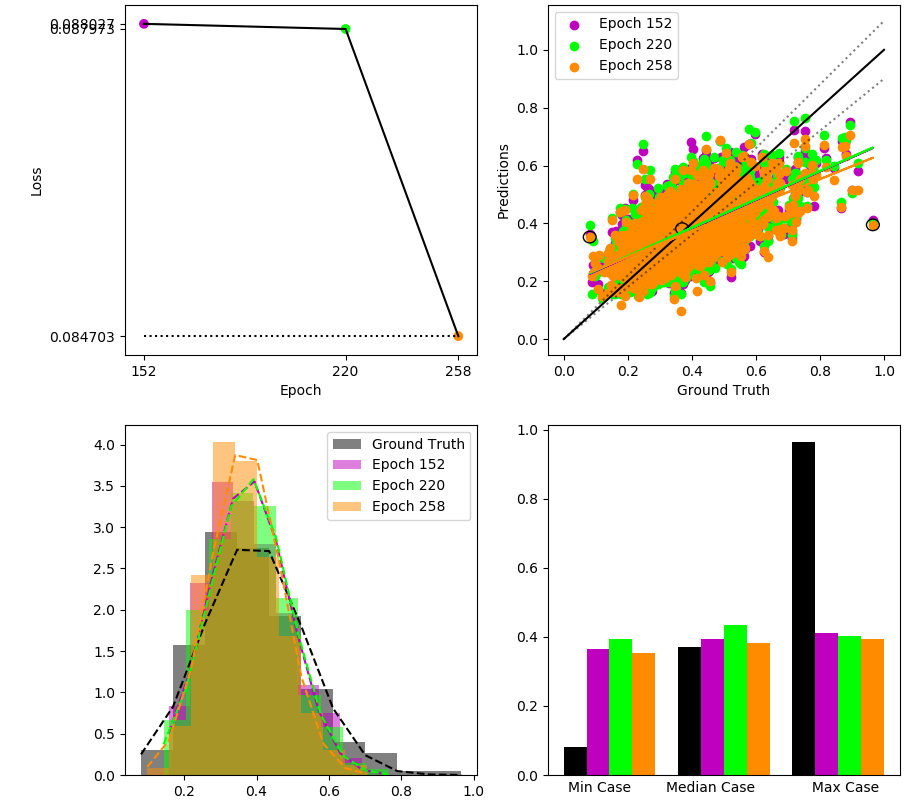
\includegraphics[scale=0.7]{Figures/transfer3.png}
	\caption{Results Dashboard for VGG19 Model with added Dropout Layer (30\%).}
	\label{fig:results_transfer}
\end{figure*}

\noindent
Over all, the transfer learning models produced inferior results to those of an architecture developed from scratch. However, the transfer learning models still provided comparable results and may have superior results in some parts of the data-range, particularly the lower part.

\section{Whole Core Experiment}

As mentioned in subsection~\label{data:outputs}, the output of Parmec is multi-dimensional, with 6 directional/rotational outputs for all 4173 interstitial bricks, with each of these values output at all 271 time frames during the earthquake. In this experiment, a single time frame was selected (frame 48) and one output metric (displacement in the West-East direction). The rationale for selecting these outputs starts by examining and comparing Figures~\ref{fig:results1} \& \ref{fig:results2}, as well as Figures~ref{fig:histo1} \& ref{fig:histo1}. Displacement in the South-North direction was discarded as limited variability can be seen looking at individual cases and at the distribution of the dataset as a whole. Looking at individual cases of displacement in the West-East direction, it can be seen that there is variability between cases (top row of Figure~\ref{fig:results1}). Also, there are a reduced number of outliers (Cyan in Figure~\ref{fig:histo1}) compared to outputs for the other time frames. 
\\

\noindent
With our selection of output data, a machine learning model was trained for 200 epochs to predict displacement in the West-East direction at frame 48 for all 4173 interstitial bricks. A visualisation of the test set predictions for a single instance can be seen in Figures~\ref{fig:preds_layer_7} \& \ref{fig:preds_layer_10}. These figures visualise the predictions of the model at the half way point of training and after the final epoch, comparing each to the ground truth.
\\

\begin{figure*}[p]
	\centering
	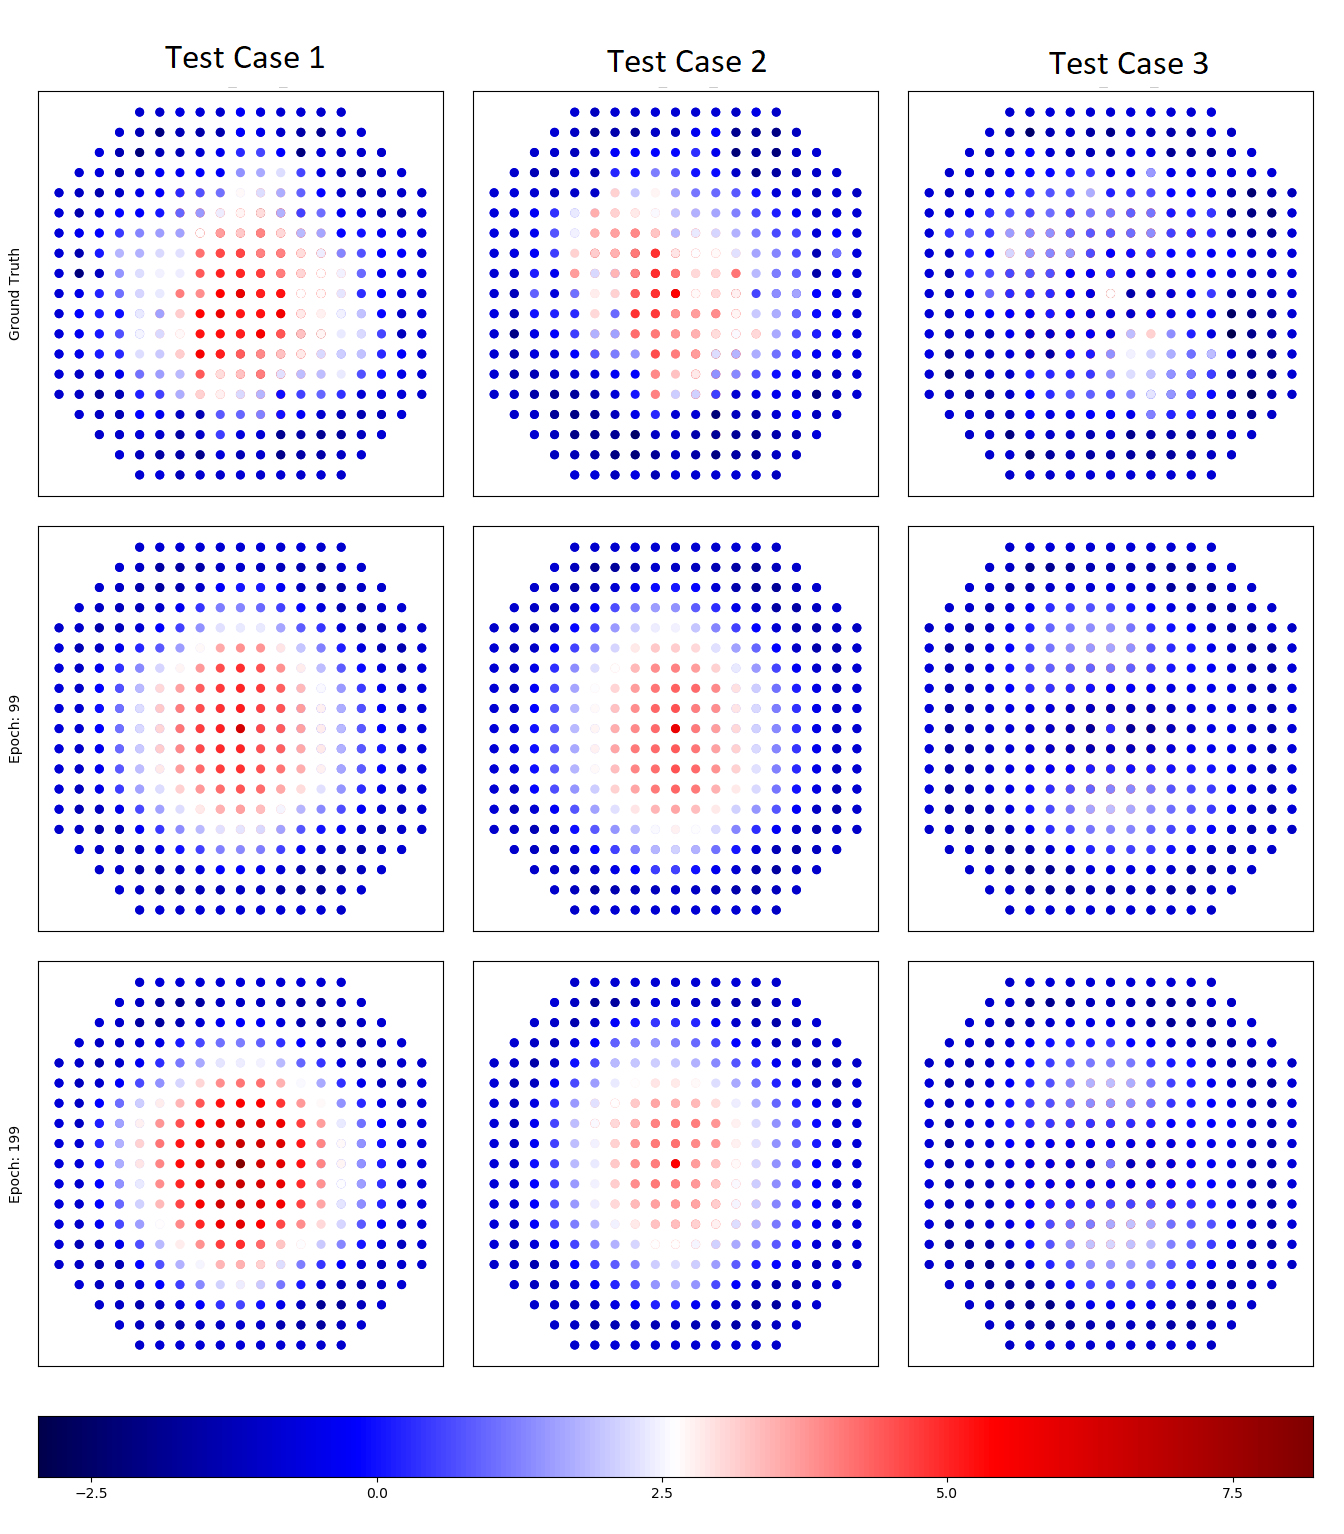
\includegraphics[scale=0.45]{Figures/preds_layer_7.png}
	\caption{Direct comparison of model predictions against ground truth labels for core level 7} {This comparison is made for predictions on the test data-set and at two points during the training process. Each column represents a different example case from the testing data-set. The top row represents the ground truth labels with the two subsequent rows showing the predictions of the model at epoch 100 and 200 (final epoch). }
	\label{fig:preds_layer_7}
\end{figure*}

\begin{figure*}[p]
	\centering
	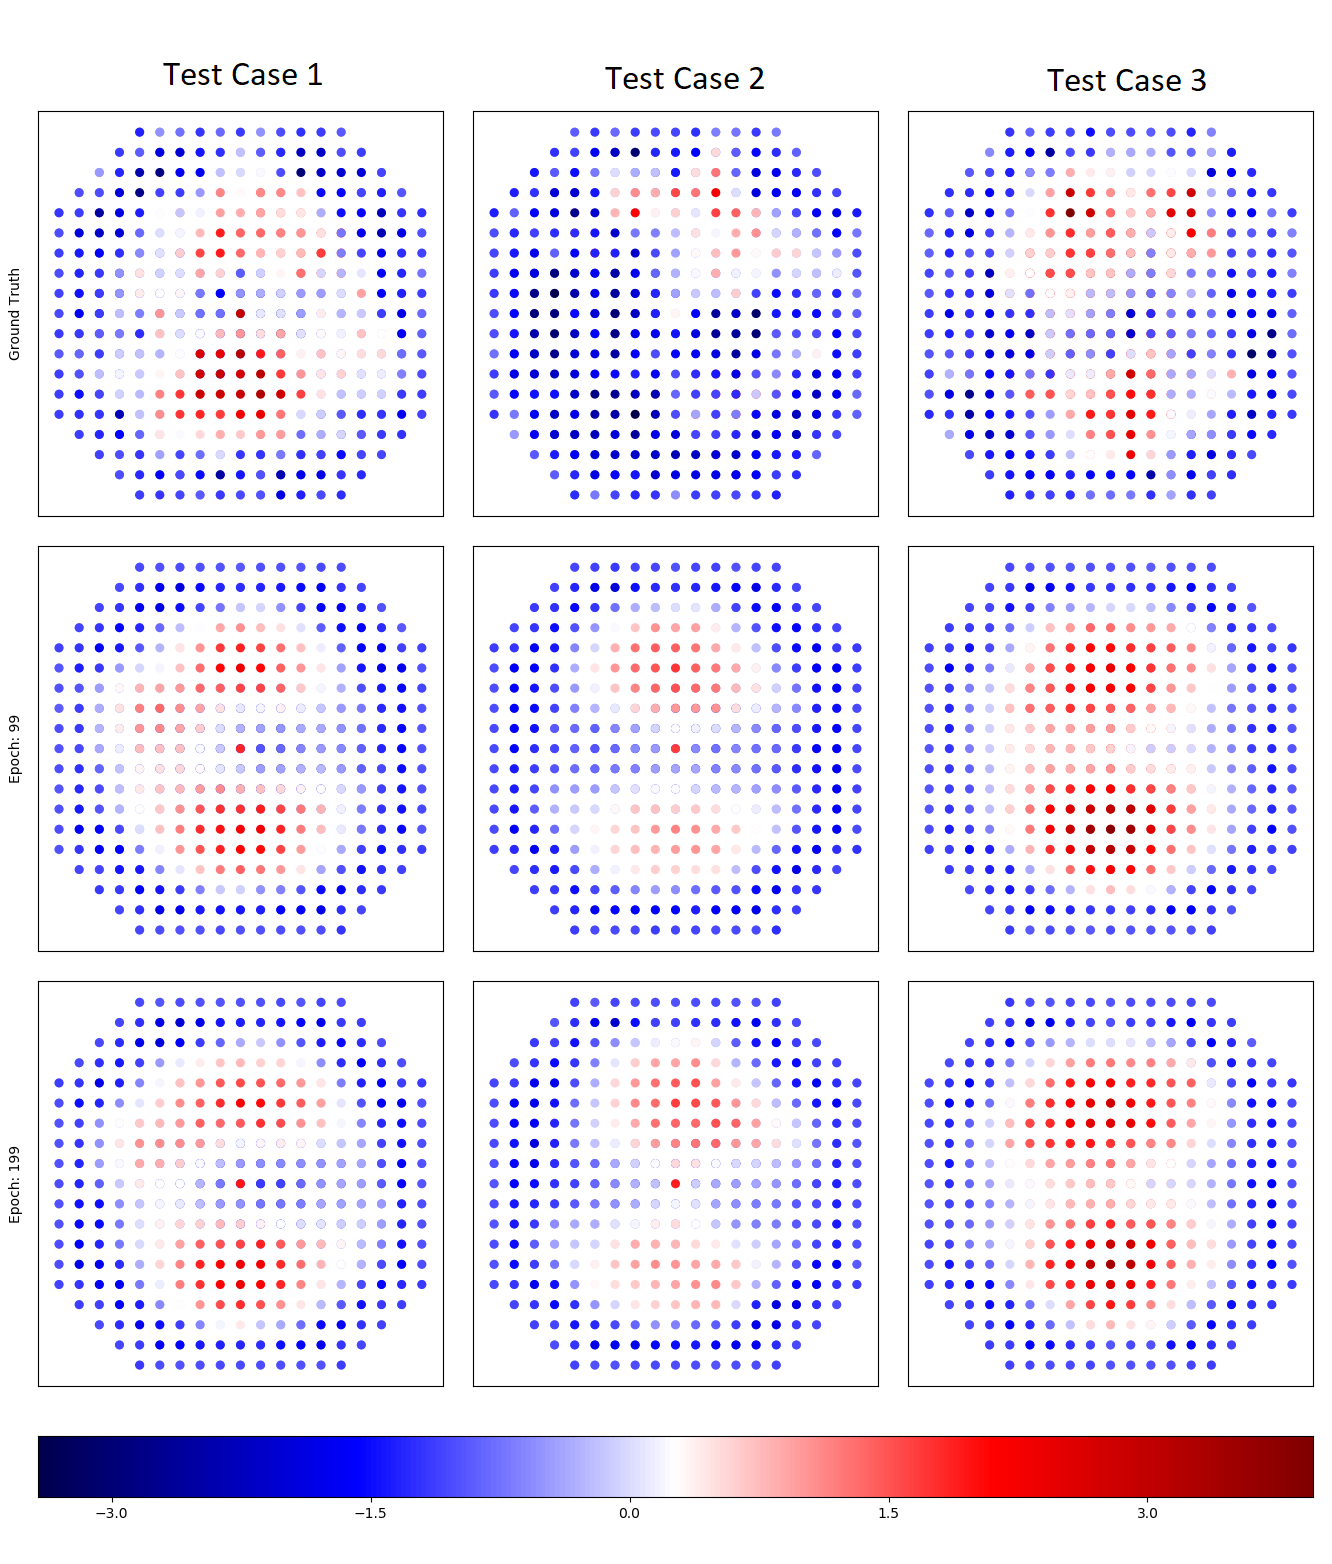
\includegraphics[scale=0.45]{Figures/preds_layer_10.png}
	\caption{Direct comparison of model predictions against ground truth labels for core level 10} {This comparison is made for predictions on the test data-set and at two points during the training process. Each column represents a different example case from the testing data-set. The top row represents the ground truth labels with the two subsequent rows showing the predictions of the model at epoch 100 and 200 (final epoch). }
	\label{fig:preds_layer_10}
\end{figure*}

\noindent
It can be seen that the model makes similar predictions for all three cases i.e. there is limited variability between the predictions. This suggests the model has a high level of bias and is not able to generalise well. The explanation for this can likely be found in the discussion within subsection \ref{correlation}, where it was revealed that the outputs for disparate regions of the core do not correlate well with each other. Therefore, this result suggests that the development of a machine learning model with the intention of predicting the displacement of all 4173 bricks may be highly complex and take considerable effort in model optimisation. Therefore, the development of a model with a narrower output prediction scope first may be a more reasonable short term goal.

\chapter[Surrogate ML Model Development]{A surrogate machine learning model for advanced gas-cooled reactor graphite core safety analysis}


\label{cha:surrogate}


This chapter is adapted from the academic article \textit{A surrogate machine learning model for advanced gas-cooled reactor graphite core safety analysis} published in the journal of Nuclear Engineering and Design \cite{jones2022surrogate}. It details the development of a machine learning model intended to surrogate the functions of the traditional engineering model Parmec \cite{wiki:xxx} used for advanced gas-cooled reactor safety analysis.

\section{Abstract}

A surrogate machine learning model was developed with the aim of predicting seismic graphite core displacements from crack configurations for the advanced gas-cooled reactor. The model was trained on a dataset
generated by a software package which simulates the behaviour of the graphite core during a severe earthquake.
Several machine learning techniques, such as the use of convolutional neural networks, were identified as highly
applicable to this particular problem. Through the development of the model, several observations and insights
were garnered which may be of interest from a graphite core analysis and safety perspective. The best performing
model was capable of making 95\% of test set predictions within a 20 percentage point margin of the ground
truth.

\section{Research Highlights}

There were three main highlights to this research article:

\begin{enumerate}
	
\item A surrogate machine learning model was developed
which aims to predict seismic graphite core displacements from crack configurations for the advanced gas-
cooled reactor. The model was trained on a dataset generated by a software package which simulates the behaviour of the graphite core during a severe earthquake.
The main motivation behind this research was to increase the computational efficiency of seismic displacement output data generation in order to allow a wider
search of the vast problem space. 

\item Following the training process of the models, the generation of output values takes less than one second. Using the same hardware, the equivalent data generation time would be over
2 hours using the original Parmec software.
The best performing model was capable of making
95\% of test set predictions within a 20 percentage point
margin of the ground truth. 

\item Through a process of feature selection i.e. reducing the expression of certain parts of the data space, engineering insights into the underlying nature of the dataset and problem can be inferred. For example, optimal model performance was observed when including input information from only the top three levels of the graphite core. From this, we can conclude that information regarding the bottom of the graphite core may be irrelevant to the prediction of displacement outputs. The feature selections identified not only are useful in the production of machine learning models, but may also be useful in a wider context i.e. engineering safety analysis in this field.


\end{enumerate}


\section{Introduction and Background}

Much of what is contained in the introductory and background sections of the journal article discussed here has already been covered in this thesis. Rather than repeat this information, the relevant sections shall simply be referred to here.

\begin{enumerate}
	
	\item Information concerning the underlying engineering problem, the advanced gas-cooled reactor (AGR) and the traditional engineering model Parmec used to perform safety analysis for the AGR is discussed in chapter~\ref{cha:engineering}.
	
	\item Regarding background information on the workings of machine learning methods, models and concepts is available in chapter~\ref{cha:ML}.
	
	\item A discussion and exploration of the dataset is given in chapter~\ref{cha:dataset}, with the programmatic framework developed to create datasets and streamline machine learning model production detailed in section~\ref{framework}.
	
	
	
\end{enumerate}

\section{Data Selection and Focus} \label{data_selection}

As explained in subsection~\ref{data:outputs}, each Parmec case contains approximately 6.8 million output parameters. For the purpose of this work,  this large data space was narrowed down into a usable format. The process of data selection was informed by the preliminary experiments reported in Chapter~\ref{cha:preliminary} and the data visualisation process from section~\ref{data:visualisation} .  
\\

\noindent
Of the six output metrics, a single displacement metric was chosen (displacement translation along the horizontal axis in the direction of the applied earthquake acceleration) at a single time frame (time frame 48 - approximately 3.8 seconds into the simulated earthquake). The justification for this selection is made at the start of section~\ref{prelim:whole} and can be summarised by examining Figure~\ref{fig:earthquake}. It can be seen that the earthquake is well underway at this point and the data from later time-steps was found to have a greater level of homogeneity and less variation between instances.
\\

\noindent
The output space was further narrowed to include data for just a single brick at a time i.e. a single label value for each instance. The selection of outputs allows the research problem to be expressed as single label regression (as opposed to multi label regression where we would attempt to predict multiple outputs per instance). The decision to focus on only a single brick and not outputs for the whole go was again made based on the findings of the preliminary experiment detailed in section~\ref{prelim:whole} where unsatisfactory results were achieved from training a model to predict outputs for all interstitial bricks. It was also discussed in subsection~\ref{correlation} that outputs for interstitial bricks poorly correlate with each other, particularly when the bricks are from geographically remote parts of the core.
\\

\noindent
The brick chosen was the one located at the upper most level at the centre of the core. This position of this brick is shown in the lower part of Figure~\ref{fig:pos_distr}. This brick is at a particularly important position from an engineering perspective. On average, the closer a channel is to the centre of the core, the higher its translational displacement relative to the surrounding structure (see Figure~\ref{fig:composite} from subsection~\ref{data:entire}). The upper level may also be considered of greater importance than those lower down, as it is the initial point of entry for a control rod. The decision to choose this brick was also informed by literature concerning engineering assessments of the AGR (see section~\ref{engineering:literature}).
\\

\noindent
The distribution of horizontal displacement at time frame 48 for all ~8300 instances is shown as a histogram in the upper part of Figure~\ref{fig:pos_distr}. It can be seen that the labels take the form of a Gaussian distribution, but with the modal value to the left of the median and mode. The data also has a long tail on the right hand side i.e. there are a number of outliers on the upper end of the distribution.

\begin{figure*}[p]
	\centering
	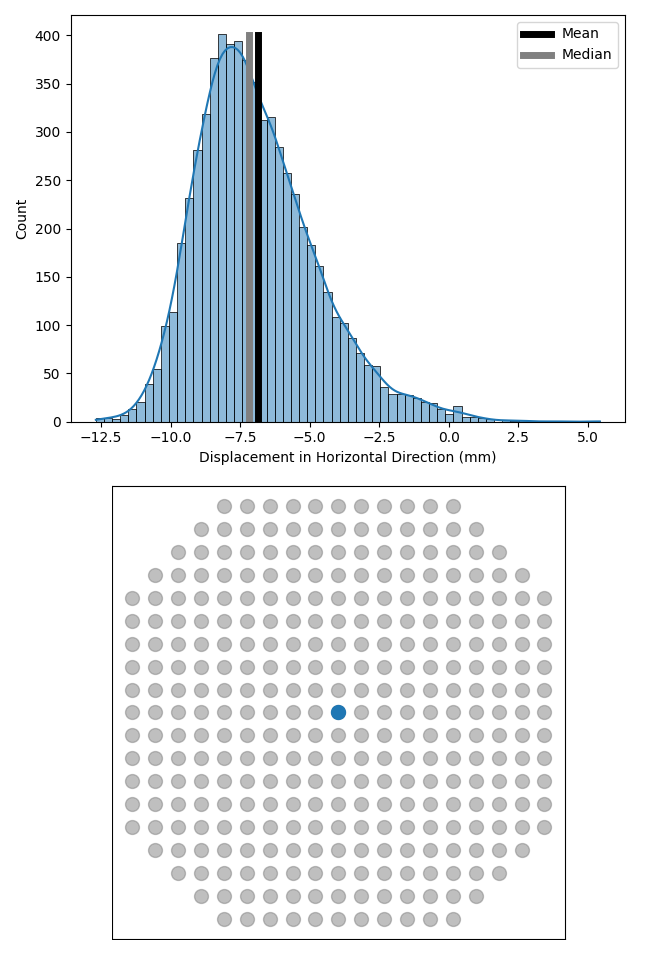
\includegraphics[scale=0.7]{Figures/position_distribution.png}
	\caption{The Position in the core from which the labels are representative of (\textbf{Bottom}); Distribution of ~8300 values in the label set (\textbf{Top})}
	\label{fig:pos_distr}
\end{figure*}

\section{Surrogate Model Development and Design} \label{method}

\subsection{Traditional Methods} \label{traditional}

We began with the use of traditional machine learning models, otherwise known as shallow methods. The methods used included: linear regression, Huber regression, support vector machines \cite{smola2004tutorial} and decision tree regression \cite{navada2011overview}. Each model type was optimised using the training set (N) followed by evaluation against the test set ($N_t$). 

\subsection{Neural Networks}

The remainder of this section discusses the development of experiments involving neural networks. Two types of neural network architecture were employed: dense neural networks (also known as fully connected networks) and convolutional neural networks.
\\

\noindent
To this end, each experimental configuration of parameters was evaluated by training a model using 10-fold cross-validation \cite{refaeilzadeh2009cross}. To account for the stochastic nature of model training caused by the random initialisation of model weights, the training process was repeated 32 for each cross-validation fold. At the start of training, a learning rate of 5.00E-04 was employed, with this being programmatically halved each time a performance plateau is detected (no validation loss improvement for 50 epochs). Early stopping \cite{yao2007early} was used when the learning rate drops below  1.00E-05, with training terminated and the parameters retained from the point at which lowest validation loss was achieved. Each optimised model was then evaluated against the test set of 2000 samples. A graphical representation of this process is seen in Figure~\ref{fig:train_history}. 
\\

\noindent
The next subsection discusses the general process of hyper-parameter optimisation during model design. The subsection after that discusses differing data input encoding shapes and the model architectures they require. Finally in this section, we discuss the impact of feature selection i.e. reducing the input feature space provided to the model.

\begin{figure}[h]
	\centering
	\includegraphics[scale=0.55]{Figures/Training History.png}
	\caption{Example of Model Training and Validation with Early Stopping and Model Saving} {As can be seen, the best model performance is produced on epoch 244 where a validation loss of 0.97 is obtained. After training for another 50 epochs, training is terminated, as in this case minimum training rate has already been achieved. The optimal model weights are then retained to evaluate against the test set.}
	\label{fig:train_history}
\end{figure}

\subsection{General Hyper-Parameters}

As mentioned in subsection~\ref{NN}, several hyper-parameters must be chosen for a neural network. The optimal selection of hyper-parameters were chosen through an experimental processes. 
\\

\noindent
The first parameter that was chosen was the optimiser. After evaluating several optimiser algorithms, including the RMSprop, Adagrad, and SGD configurations, the Adam optimiser with Nesterov momentum \cite{dozat2016incorporating} was was chosen as it provided the best model performance.
\\

\noindent
Three model additional model hyper-parameters were also refined: nodal architecture, activation functions and regularisation. Starting with the architecture, this was developed through a trial and error method. Beginning with a simple structure of a single hidden layer with a width of four nodes, this was then expanded and adjusted experimentally, using the testing loss for each configuration as a measure of its performance. Guidance was taken from previous works as to what architectures may be most effective, including \cite{fernandez2017nuclear} which describes four distinct architectures which were used as a starting point for the experiments performed here. 
\\

\noindent
In tandem with the nodal architecture, the use of activation functions were chosen experimentally. At first, the same activation function was applied to each layer (bar the output layer). The use of three commonly employed activation functions were tested: sigmoid, the rectified linear unit (ReLu) \cite{hara2015analysis} and the hyperbolic tangent function \cite{kalman1992tanh}. Also tested was the less common softplus function \cite{zheng2015improving} which has been used in other surrogate model works, including \cite{liang2018deep}. In addition to a model design that uses the same activation function in all layers, alternative configurations were tested . Initially, a method employing non-linear activations on every other layer was employed, with the alternating layers simply outputting the linear combination of inputs and weights. Inspiration for this approach was taken from \cite{ahn2020deep} where non-linear activations were only placed on every 4th layer of the neural network architecture. This was further modified to an architecture employing two different non-linear activation functions in the same model, with the greatest success being observed when alternating softmax and tanh. The final model, demonstrating the optimal architecture, is shown in Figure~\ref{fig:model_architecture}.
\\

\noindent
The regularisation parameter was also optimised experimentally. The most effective technique was found to be dropout \cite{srivastava2014dropout} where the output of randomly selected layers are negated. It was determined experimentally that a dropout parameter of 0.4 was optimal - the output of 40\% of the nodes in each layer were randomly dropped. 
\\

\noindent
The experimental models were trained using several loss functions. These were mean squared error (MSE) mean absolute error (MAE) and the Huber loss \cite{huber1964robust}. By inter-comparing each loss function, it was found that Huber was the optimal loss function for training the model.


\begin{figure*}[h]
	\centering
	\includegraphics[scale=1.2]{Figures/architecture_final.png}
	\caption{The Final Architecture of the Model}
	\label{fig:model_architecture}
\end{figure*} 

\begin{figure*}[p]
	\centering
	\includegraphics[scale=0.8]{Figures/convo_proj2.png}
	\caption{Convolution on a 2-dimensional Input Space Using a 3x3 Filter} {The input space is a top-down cross-sectional slice of a 3-dimensional tensor. This represents the distribution of cracks in a single level of the AGR reactor for a single example. The corners and edges have been padded with zeros to maintain a regular shape. The convolutional operation has been performed at select locations. \textbf{Lower-right}: the patch from the input space is the perfect inverse of the filter, resulting in the lowest possible output value (-9). \textbf{Left}: the input patch is a perfect match of the filter, resulting in the maximum output (9). \textbf{Top-right}: a middling example where the input patch has only a slight resemblance to the filter. Outside of the image on the top right-right hand corner, the mathematical operation between a data patch and filter is seen: both are flattened into a vector followed by a dot product calculation. }
	\label{fig:convo_operation}
\end{figure*} 

\begin{figure*}[p]
	\centering
	\includegraphics[scale=0.7]{Figures/convo_vis.png}
	\caption{Convolution on a Single Instance Encoded in a 3-dimensional Format Using an Example Multi Channel Filter} {\textbf{Top}: a single instance encoded with each core level represented as a separate channel. \textbf{Left}: a single filter from the first layer of a CNN, the planar dimensions are smaller than the input space (3x3), but the number of channels are equal to the number in the input space (7). The filter performs the mathematical operation shown in Figure~\ref{fig:convo_operation} on each channel. The sum of all channels operations forms a single value in the output feature map for this filter. \textbf{Right}: the feature map for the filter. If the aforementioned mathematical operation is performed across the entire input space, we get the feature map shown here. If this process is performed for multiple filters, several feature maps are produced, which each represent channel inputs for the next convolutional layer. Alternatively, the feature map can be flattened as to form the input for a dense layer). }
	\label{fig:feature_maps}
\end{figure*}


\newpage
\subsection{Neural Network Input Encoding} \label{encoding_method}

Three alternative configurations of neural network were employed, each requiring a differing data encoding format, as outlined in the following subsections. One of these configurations employs only dense neural network architecture, with the other two employing convolutional neural network architecture.  An experiment was designed to compare each of these encoding formats in turn.
\\

\noindent
In each case, the number of input features is the same: 1988 (the number of fuel bricks). Similarly, there is a single output (the displacement for the central interstitial brick in the top level). In each case, a similar model architecture is used, with notable exceptions such as the use of only dense layers or the inclusion of convolutional layers.

\begin{table}[h!]
	\begin{center}
		
		\begin{tabular}{c|c|c|r|c} % <-- Alignments: 1st column left, 2nd middle and 3rd right, with vertical lines in between
			\textbf{Encoding} & \textbf{Input} & \textbf{Output} & \textbf{Model} \\
			
			\textbf{Mode} & \textbf{Format} & \textbf{Shape} & \textbf{Architecture} \\
			\hline
			1D & 1988 & 1 & DNN Only \\
			2D & 7 x 284 &  1 & CNN \& DNN \\
			3D & 7 x 20 x 20 &  1 & CNN \& DNN \\
			
		\end{tabular}
		\caption{Summary of the Input Encoding Experiment} {For each encoding format, the total size of the input is the same; only the shape changes. Additionally, the output label in each case is the same shape. Note also that the 1D encoding requires a model containing only dense layers, whereas 2D and 3D encoding warrants a mix of convolutional and dense layers. }
		\label{tab:encodings}
	\end{center}
\end{table}

\subsubsection{DNN - 1D}

A dense neural network with 1D encoding is employed. In this configuration, the data is encoded in the base format as mentioned in subsection~\ref{data:inputs} where each instance is input to the model as a vector. In the DNN, the output of each layer is fed into all nodes of the subsequent layer.

\subsubsection{CNN - 2D}

A convolutional neural network architecture with 2D encoding. In this format a 2-dimensional filter is applied at select patches on a 2-dimensional input space (Figure~\ref{fig:convo_operation}). To facilitate this, the 1988 element long input feature vector is reshaped into a matrix. The dimensions of this matrix are 7 by 284: the bricks per fuel channel (BFC) by number of fuel channels (NFC), respectively. Hence, in this encoding format, an individual instance has a feature matrix of the form $\textbf{x}_i~=~\{-1, 1\}^{BFC \times NFC}$. This format is analogous to CNNs used for image recognition which use a grey-scale bitmap as input \cite{bui2016using}. 
\\

\noindent
The architecture produced during the DNN optimisation was kept the same. However, the first 5 layers now became CNN layers with the latter two remaining fully connected layers. This resulted in an additional parameter to be optimised: the size of the convolutional window shape (or kernel). A window size of 3 by 3 was experimentally found to produce the best result.

\subsubsection{CNN - 3D} A convolutional neural network architecture with 3D encoding. This arrangement reflects the true positional relationship within the actual core. The bricks are stacked in 7 levels (BFC). At its widest width and breadth, the core is 18 channels across. The tensor has been padded at the edges and corners with zeros to make it a regular shape and keep the input shape the same size in subsequent layers \cite{dwarampudi2019effects}. Consequently, CW \& CB both have a value of 22 due to a double layer of zeros on each side. Therefore the dimensions of this input tensor are bricks per fuel channel (BFC) by core width (CW) by core breadth (CB): 7 by 20 by 20 i.e the input features for each instance is in the form $ \textbf{x}_i~=~\{-1, 0, 1\}^{BFC \times CW \times CB}$. This input shape can again be used by a CNN with a 2-dimensional architecture. However, with a 3-dimensional encoding each core level is used as a separate input channel. In this format, the filter has multiple channels, one for each of the channels in the input space (see Figure~\ref{fig:feature_maps}). This is analogous to CNNs used for image recognition where colour data (usually red, green and blue) are represented by different input channels \cite{albawi2017understanding}. 

\subsection{Feature Selection} \label{feature_selection}

In section~\ref{data}, it is mentioned that the input to Parmec is a vector 1988 elements long, each representing the cracking status on one bricks in the model. So far in this section, we have discussed various dimensional encoding formats available, including a 3-dimensional encoding which represents the true physical arrangement of the core. We have the choice to provide this information to the model in its entirety, or to reduce the scope of these inputs in some way. Through a process of feature selection \cite{gurney1997introduction}, we can actively chose only the most relevant features to the predicted output by monitoring the model performance as the scope is adjusted. Beyond model performance optimisation, the process of feature selection allows insights into the data, including relationships between inputs and outputs, what information is relevant and so on. As mentioned in subsection~\ref{framework}, the framework developed for this research work allows the selection of features programmatically. 
\\

\noindent
The proposed method for feature selection is to split the core in different ways and then perform experiments using only those features. Two differing strategies are discussed in the following sections.

\subsubsection{Regional Selection} \label{regional_selection}

The core features are split into concentric sections as shown in Figure~\ref{fig:regions}.  Recall that the value we aim to predict is for the central channel (Figure~\ref{fig:pos_distr}). Hence each concentric region is effectively further removed from the position of interest. It can be hypothesised that the data for regions closer to the central position are most important to model performance, with importance falling as we move further away. Testing this hypothesis is the purpose for this experiment.
\\

\noindent
Starting with the greater core region (i.e. the whole feature set) a model is trained and evaluated.The feature set is then reduced by incrementally removing channel regions and then training a new model using it. By repeating this process until only the inner channel region remains and evaluating the trained model at each stage, we can choose the optimal features for inclusion.

\begin{figure}[h]
	\centering
	\includegraphics[scale=0.7]{Figures/core_regions.png}
	\caption{The Core Separated into Regions for the Purpose of Feature Selection} {The method of this experiment is discussed in Subsection~\ref{regional_selection} with the results given in Table~\ref{tab:regional}. }
	\label{fig:regions}
\end{figure}

\subsubsection{Level Selection} \label{level_selection}

In addition to feature selection based on the core regions from, the feature set was also varied in size by varying the number of core levels (refer back to Figure~\ref{fig:schematic}). Recall from section~\ref{data_selection} that the brick for which we are attempting to predict displacement values for is in the top layer. Similar to the experiment in the previous subsection, is can be conjectured that the lower levels of the core are less important than those near the top (closer to the point of interest). This again was determined experimentally. Starting with the lowest level (level 1), data for incrementally higher core levels was removed from the feature set, training and evaluating the model each time. 



\section{Results} \label{results}

\subsection{Traditional Methods}

As mentioned in subsection~\ref{traditional}, the experimental processes for this work began with the use of traditional machine learning methods. The results are summarised in Table~\ref{tab:traditional}. As can be seen, the linear regression method produces the best test loss and therefore best performing model. This is followed by the Huber and support vector regression methods. A decision tree regression model can fit the the training data almost perfectly (a training loss of zero). However, the decision tree regression model also performs worst on the testing set, suggesting overfitting.  

\begin{table}[h!]
	\begin{center}
		
		\begin{tabular}{c|c|c|r|c} % <-- Alignments: 1st column left, 2nd middle and 3rd right, with vertical lines in between
			\textbf{Inclusive} & \textbf{Training} & \textbf{Test} \\
			
			\textbf{Levels} & \textbf{Loss} & \textbf{Loss} \\
			\hline
			Linear Regression & 7.2e-3 & 1.2e-2 \\
			Huber Regression & 7.7e-3 &  1.3e-2 \\
			Support Vector Regression & 5.8e-3 &  1.4e-2 \\
			Decision Tree Regression & 0 & 4.7e-2 \\
		\end{tabular}
		\caption{Summary of the Test Results from the Traditional Methods Experiment (Subsection~\ref{traditional})} {Values are in mean squared error (MSE). }
		\label{tab:traditional}
	\end{center}
\end{table}


\subsection{Input Encoding} \label{encoding_results}

Table~\ref{tab:encoding} summarises the results of the experiment outlined in subsection~\ref{encoding_method}, with the best result achieved with each encoding format shown. \\

\begin{table}[h!]
	\begin{center}
		
		\begin{tabular}{c|c|c|r|c} % <-- Alignments: 1st column left, 2nd middle and 3rd right, with vertical lines in between
			\textbf{Encoding} & \textbf{Lowest} & \textbf{Mean} \\
			
			\textbf{Format} & \textbf{Loss} & \textbf{Loss} \\
			\hline
			3D (CNN) & 9.9e-3  & 1.3e-2 \\
			2D (CNN) & 1.1e-2  & 1.6e-2 \\
			1D (DNN) & 1.3e-2 & 1.3e-2 \\
		\end{tabular}
		\caption{Summary of the Test Results from the Input Encoding Experiment (Subsection~\ref{encoding_method})} {Values are in mean squared error (MSE). Each part of the experiment was repeated 32 times for each cross validation fold (320 total) with starting weights initialised randomly each time. The weights were stored at the optimal point during training (lowest validation loss). Each saved model was then evaluated against the test set of 2000 samples, with the lowest and mean values reported in this table.}
		\label{tab:encoding}
	\end{center}
\end{table}

\noindent
From the results, it can be seen that a CNN employing 3D data encoding produces the best performance. In turn, it can also be seen that a CNN employing 2D encoding produces a lower overall loss value than a DNN employing 1D encoding. See subsection~\ref{analysis} for further discussion of these results. 

\subsection{Feature Selection} \label{feature_extract_results}

Recall from subsection~\ref{feature_selection} that two strategies are proposed for experimental feature selection: regional and level selection. 
\\

\noindent
Table~\ref{tab:regional} summarises the results for the regional feature selection experiment (subsection~\ref{regional_selection}). Each row represents a model trained using the data for channels inclusively within the region indicated. For example, Main Core (green in Figure~\ref{fig:regions}) includes data for itself and the regions internal to it (central and inner) but not the region beyond it (greater core). 
\\

\begin{table}[h!]
	\begin{center}
		
		\begin{tabular}{c|c|c|r|c} % <-- Alignments: 1st column left, 2nd middle and 3rd right, with vertical lines in between
			\textbf{Inclusive} & \textbf{Lowest} & \textbf{Mean} \\
			
			\textbf{Regions} & \textbf{Loss} & \textbf{Loss} \\
			\hline
			Greater Core (blue) & 9.9e-3  & 1.3e-2 \\
			Main Core (green) & 1.6e-2 & 1.7e-2 \\
			Central (yellow) & 2.0e-2 & 2.2e-2  \\
			Inner (red) & 2.1e-2 & 2.3e-2  \\
		\end{tabular}
		\caption{Summary of the Test Results from the Regional Feature Selection Experiment (Subsection~\ref{regional_selection})} {Values are in mean squared error (MSE). Each part of the experiment was repeated 32 times for each cross validation fold (320 total) with starting weights initialised randomly each time. The weights were stored at the optimal point during training (lowest validation loss). Each saved model was then evaluated against the test set of 2000 samples, with the lowest and mean values reported in this table.}
		\label{tab:regional}
	\end{center}
\end{table}

\noindent
Table~\ref{tab:levels} summarises the results for the regional feature selection experiment (subsection~\ref{level_selection}). Each row represents a model trained using the data for channels inclusively within the levels indicated.
\\

\begin{table}[h!]
	\begin{center}
		
		\begin{tabular}{c|c|c|r|c} % <-- Alignments: 1st column left, 2nd middle and 3rd right, with vertical lines in between
			\textbf{Inclusive} & \textbf{Lowest} & \textbf{Mean} \\
			
			\textbf{Levels} & \textbf{Loss} & \textbf{Loss} \\
			\hline
			5 - 7 & 9.6e-3 & 1.1e-2 \\
			3 - 7 & 9.7e-3 & 1.2e-2 \\
			4 - 7 & 9.8e-3 & 1.2e-2 \\
			2 - 7 & 9.8e-3 & 1.2e-2 \\
			1 - 7 & 9.9e-3 & 1.3e-2 \\
			6 - 7 & 1.1e-2 & 1.3e-2 \\
		\end{tabular}
		\caption{Summary of the Test Results from the Level Feature Selection Experiment} { Values are in mean squared error (MSE). Each part of the experiment was repeated 32 times for each cross validation fold (320 total) with starting weights initialised randomly each time. The weights were stored at the optimal point during training (lowest validation loss). Each saved model was then evaluated against the test set of 2000 samples, with the lowest and mean values reported in this table (Subsection~\ref{level_selection}).}
		\label{tab:levels}
	\end{center}
\end{table}

\noindent
From Table~\ref{tab:regional}, it can be seen that including features from the whole core produces the best result. From Table~\ref{tab:levels} it can be seen that the optimal result is achieved when including levels 5 - 7. See subsection~\ref{analysis} for further discussion of these results.

\begin{figure*}[h]
	\centering
	\includegraphics[scale=0.55]{Figures/region_compare2.png}
	\caption{Visual Summary of the Regional Feature Extraction Experiment} {\textbf{Top:} the concentric core regions as described in Figure~\ref{fig:regions} with two inclusive regions delineated which represent the features included in the models corresponding to the mid and bottom image. \textbf{Mid:} The distribution of predictions made by a model trained on features representing the central two regions (red and yellow in the image above). It can be seen that the distribution of predictions in the upper end of the histogram is similar to that of the ground truth. However, this model makes few predictions in the lower region of the distribution, effectively overestimating these results. \textbf{Bottom:} When including all regions in the feature set, superior model performance is seen. The shape of the distribution for the model predictions closely fits that of the ground truth. }
	\label{fig:central}
\end{figure*}

\subsection{Analysis and Discussion} \label{analysis}

Looking at the final model architecture 
(Figure~\ref{fig:model_architecture}), it can be seen that considerable complexity must be employed in terms of model parameters to produce the optimal result. This suggests that relationships between inputs and outputs are complex. This is to be expected, as the Parmec model is itself highly complex involving thousands of equations and parameters.
\\

\noindent
From Table~\ref{tab:encoding}, it can be seen that CNN architecture produces superior results to DNNs. Encoding the input features in a 3-dimensional format produces the best results. In addition, neural network models perform better than traditional methods as seen in Table~\ref{tab:traditional}. This suggests that true physical relationships within the data, i.e. local 3-dimensional configurations of cracks, have a causal relationship with displacements.
\\

\noindent
During the feature extraction experiment, it is noteworthy that the best result was achieved when including features representing all core regions, including the most distant, outer regions far removed from the location of the central channel. It was conjectured earlier that only the channels most local to the position of interest (the centre) would be of importance to predicting displacement. However, from Table~\ref{tab:regional} it can be seen that model performance drops sharply when excluding data for the main core channels. This suggests that cracking beyond the local region has a causal effect on the central channel's displacement. This phenomena is particularly interesting when considered along with the fact that the optimal convolutional window size is 3x3 (a relatively small window size by CNN standards) which suggests small patterns are most important.
\\

\noindent
Looking more closely at the results of this experiment, Figure~\ref{fig:central} shows the distribution of predictions made by models trained on the channels within the central core and full core. It can be seen that a model that excludes the main and greater core channels has difficulty making predictions in the lower part of the prediction spectrum. Perhaps the cracking status of bricks beyond the central core has some slackening or tightening effect on the centre of the core. The exact reason for this phenomenon will require further study.
\\

\noindent
Examining the results of the experiment which excludes features by core levels (Table~\ref{tab:levels}), it can be seen that the best overall result is achieved when including features for the top three levels (5~-~7). Note also that a similar performance is achieved with all arrangements except when only the top two levels were included (6~-~7), hence low sensitivity. From these results, we can conclude that the at least the top three levels have a discernible impact on the displacement of the central core channel.
\\

\noindent
Figure~\ref{fig:best_margins} shows the test predictions for the best performing model (3D CNN trained on features for levels 5-7) plotted against the ground truth. It can be seen that 94.8\% of the test predictions fall within a margin of 20\%  of the ground truth in absolute terms. Of the cases that fall outside this margin, we can see that most of them occur fairly close to the boundary. Using the same process as was used to generate this plot, we can identify the type of case which is difficult for the model to predict accurate values for, and generate cases accordingly. From a cursory examination of the cases outside of the 20\% margin from Figure~\ref{fig:best_margins}, it was observed that they contained on average 5\% fewer cracks in the top core level than the wider dataset. 
\\



\begin{figure}[h]
	\centering
	\includegraphics[scale=0.65]{Figures/best_results_distribution_margins.png}
	\caption{Model Predictions against Ground Truth for the Test Set} {A 'perfect' model would produce values on the solid black line i.e. exactly the ground truth values. Lines representing an error margin of 10 and 20 absolute percentage points of deviation can be seen. Data-points are coloured according to their deviation from the ground truth. The testing mean squared error for this model was 9e-3, with an mean absolute error of 7.4e-3. The blue line represents a linear fit with the equation 0.58x + 0.16. The $R^2$ value is 0.53. }
	\label{fig:best_margins}
\end{figure}

\begin{figure}[p]
	\centering
	\includegraphics[scale=0.47]{Figures/best_results_analysis.png}
	\caption{Model Predictions against Ground Truth for the Test Set With Values Separated into Positives/Negatives by Three Different Thresholds} {The values are then classified by whether they fall into the same half of the distribution as the ground truth. \textbf{Top:} The separator is placed as the dataset mean (0.36). \textbf{Upper Middle:} The separator is placed to the lower side of the modal value. \textbf{Lower Middle:} The separator is placed just before a region of outlier values. \textbf{Bottom:} The dataset distribution for context.}
	\label{fig:best_analysis}
\end{figure}

\noindent
To further evaluate the performance of the model, we can separate the plot shown in Figure~\ref{fig:best_margins} into positive and negative values based on chosen thresholds. Figure~\ref{fig:best_analysis} shows the predictions and ground truth separated based on three chosen thresholds. Taking the mean as the positive/negative separator (top), it can be seen that the model performs well at predicting which region a given instance is in. However, the model performs less well at predicting values for cases at the very extremes of the data continuum (threshold of 0.2 and 0.6). Nevertheless, the 'false' examples are predicted as close to the boundary in all three graph configurations. In general, it can be seen that cases at the lower and upper ends of the data range are predicted as closer to the mean than the ground truth. Looking at the distribution of the dataset (bottom), a possible explanation is that it is highly 'biased' towards the region close to the mean i.e. the model has many fewer cases to learn from at the ends of the distribution.
\\

\noindent
Following the training process of all models discussed in this section, the generation of output values takes less than one second per instance. Using the same hardware, the equivalent data generation time would be over 2 hours using the original Parmec software.
\\

\noindent
To summarise the observations made:

\begin{enumerate}
	\item \textbf{Model Complexity:} the optimal surrogate model architecture exhibits considerable depth and width as well as requiring considerable refinement and tuning. This suggests a complex and non-trivial relationship between inputs and outputs.
	\item \textbf{Input Encoding:} optimal performance was seen when including true physical relationships in the input features i.e. a 3-dimensional encoding which represents the actual structure of the graphite core.
	\item \textbf{Feature Selection - Regional:} when selecting input features regionally by dividing the graphite core into radial segments, it was observed that optimal model performance was achieved when including data for all regions. This suggests that the cracking status of even bricks far away from the position of interest are important to the prediction of displacements. 
	
	\item \textbf{Feature Selection - Level:} when selecting input features vertically by selecting inputs from inclusive ranges of core levels, it was observed that optimal model performance was achieved when including data for the top five levels. Further, little performance sensitivity was observed when reducing the levels included in the feature dataset.
	
	\item \textbf{Difficult to Predict Cases: } cases were identified that are difficult for the model to accurately predict. Through examining these cases, some common characteristics were observed. These observations may help to design further machine learning experiments or inform engineering analysis.
	\item \textbf{Dataset Bias:} we can note that the model has lower prediction accuracy near the extremes of the data range. This can be explained by the fact that the dataset is biased towards the central region, meaning the model has fewer examples from the extremes to learn from.
\end{enumerate}


\section{Conclusion} \label{conclusion}

A surrogate machine learning model was developed which aims to predict seismic graphite core displacements from crack configurations for the advanced gas-cooled reactor. The model was trained on a dataset generated by a software package which simulates the behaviour of the graphite core during a severe earthquake. 
\\

\noindent
The main motivation behind this research was to increase the computational efficiency of seismic displacement output data generation in order to allow a wider search of the vast problem space. Following the training process of the models, the generation of output values takes less than one second. Using the same hardware, the equivalent data generation time would be over 2 hours using the original Parmec software.
\\

\noindent
The best performing model was capable of making 95\% of test set predictions within a 20 percentage point margin of the ground truth. Although this result demonstrates progress towards the development of an efficient and accurate machine learning surrogate, the high standards within the nuclear safety field mean that it is unlikely to be at a stage were it could be commercially deployed. Nevertheless, machine learning techniques were identified as highly applicable to this particular problem. For example, Convolutional neural networks were identified as more effective than other techniques available. Additionally insights into optimal hyper-parameters and inputs were also garnered. These observations may guide and support further development and progress in this area.



    

\chapter[Methods to Improve Surrogate ML Models]{Methods to Improve Surrogate Machine Learning Model Performance}
\label{cha:Improve}

\section{Abstract}

We demonstrate the adaption of three established methods to the field of surrogate machine learning model development. These methods are data augmentation, custom loss functions and transfer learning. Each of these methods have seen widespread use in the field of machine learning, however, here we apply them specifically to surrogate machine learning model development. The machine learning model that forms the basis behind this work was intended to surrogate a traditional engineering model used in the UK nuclear industry. Previous performance of this model has been hampered by poor performance due to limited training data. Here, we demonstrate that through a combination of additional techniques, model performance can be significantly improved. We show that each of the aforementioned techniques have utility in their own right and in combination with one another. However, we see them best applied as part of a transfer learning operation. Five pre-trained surrogate models produced prior to this research were further trained with an augmented dataset and with our custom loss function. Through the combination of all three techniques, we see an improvement of at least $38\%$ in performance across the five models.

\section{Research Highlights}

There were three main highlights to this research article:

\begin{enumerate}
	
	\item By adapting three existing machine learning techniques, we were able to improve model performance by at least $38\%$ over the method described in chapter~\ref{cha:surrogate}.
	
	\item This research represents a novel implementation of data augmentation, with mirroring and rotation employed in a very different way to which they are normally.
	
	\item This research also represents a novel implementation of custom loss functions. In previous research, they were used for classification problems and compensated for gaps in the data. By contrast, this research problem uses them in a regression model and compensates for a dataset concentrated around a central point.
	
\end{enumerate}

\section{Introduction}

A machine learning surrogate (MLS) is a model which aims to explain natural or mathematical phenomena which can already be explained using an existing model. Using data from the original model, machine learning techniques are used to produce an optimised MLS model. The advantages of an MLS include increased computational efficiency when generating model outputs, with the trade-off being reduced accuracy. Once developed and trained, machine learning models (including an MLS) can produce new data instances almost instantly using a standard computer, whereas generating the same information using the original model and equivalent hardware may require hours or days of computational effort. The reduction in accuracy between an MLS and an original model must be quantified on a case-by-case basis and assessed on whether it is acceptable for practical use.
\\

\begin{figure*}[h]
	\centering
	\includegraphics[scale=0.65]{Figures/MLS_vs_OM.png}
	\caption{The Trade-off Between a Machine Learning Surrogate Model and the Original Model} {Once trained on data from the original model, the production of new data is likely to be significantly more efficient in terms of computation and time. However, as the machine learning model is produced using data from the original model, there will be some inevitable reduction in accuracy.}
	\label{fig:surrogate_vs_model}
\end{figure*}

\noindent
Previous research works have dealt with the production of MLS in areas such as material properties prediction \cite{nyshadham2019machine} and \cite{asteris2021predicting}, with a recent work focusing on seismic analysis for nuclear graphite cores (see chapter~\ref{cha:surrogate}). It is the MLS model from this latest research work that will be focused on in this paper. In the aforementioned works, a strong focus on neural networks \cite{gurney1997introduction} is seen, including convolutional neural networks (CNNs).
\\

\noindent
Despite the motivation for the production of MLS models being to reduce the need for expensive production of data, a large amount of this data is required to train such a model. A machine learning model trained on an insufficient number of data instances may result in overfitting \cite{hawkins2004problem}. Some techniques were employed in the aforementioned paper, including randomised layer dropout \cite{srivastava2014dropout}, to counteract the effects of overfitting . 
\\

\noindent
A common technique used to improve model performance given a limited dataset is to manipulate existing data instances in a process known as data augmentation \cite{perez2017effectiveness}. This approach is commonly employed in machine learning applications involving image recognition and analysis \cite{hansen2015tiny}, with techniques such as mirroring and rotation used to increase the number of data instances in a dataset.
\\

\noindent
Another commonly encountered problem during machine learning model development is dataset bias. In this situation, the dataset used to train the model is weighted towards a particular region of the input and/or output space. Alternatively, the dataset may be sparse in a particular region of the data space i.e. there may only be few data examples for a part of the data input or output continuum. Several methods can be employed to counteract the problem of dataset bias, including emphasising underrepresented data samples to a greater degree. We may instead use a loss function during model training which is designed to correct for dataset bias. 
\\

\noindent
A third problem encountered when training neural networks is the computational cost associated with their development and optimisation. This is particularly problematic when the problem space is complex - such as it is in this research. Instead of starting from scratch, we may use models produced from previous research works as a starting point during the development of neural networks for our own research. Through a process of transfer learning \cite{torrey2010transfer} we can adapt the model architecture, as well as the optimised weights, generated during previous works. By using transfer learning we may be able to make our model development process more efficient by reducing the time and computational resource needed to optimise a model for our purposes. 
\\

\noindent
A research question to be investigated and answered by this paper is whether data augmentation can be applied to problems such as machine learning surrogates. To this end, a framework will be developed to apply image manipulation techniques to the dataset used in the aforementioned graphite core model. In addition, we will investigate whether the use of custom loss functions and transfer learning can improve model performance.


\section{Background} \label{Background}

\subsection{Advanced Gas-cooled Reactors and the Parmec Model} \label{Parmec}

Information concerning the underlying engineering problem, the advanced gas-cooled reactor (AGR) and the traditional engineering model Parmec used to perform safety analysis for the AGR is discussed in chapter~\ref{cha:engineering}.

\subsection{Previous Machine Learning Surrogate Model of Parmec} \label{previous}

The work that this chapter builds on is discussed in chapter~\ref{cha:surrogate}.

\subsection{Data Augmentation} \label{augmentation}


Data augmentation is frequently employed in classification problems within the field of machine learning \cite{shorten2019survey}, where the model predicts a discrete category for each dataset instance. A classic example of classification is in computer vision, where a 2D or 3D tensor representing an image is used to predict a category that is depicted. For example, models trained on the ImageNet dataset \cite{deng2009imagenet}, which contains millions of images each representing one of 1000 discrete classifications, attempt to categorise the image depicted in an instance it is presented with. Classification is in contrast to regression problems, where there is a continuous, rather than discrete, output variable.
\\

\noindent
When dealing with problems such as ImageNet classification, performance is constrained by the size of the dataset. Model performance tends to improve with a larger number of training examples. A related constraint is dataset bias: regardless of the overall number of examples in the entire dataset, if one or more classes exhibits a significantly lesser or greater number of examples than the rest, model performance may be inhibited. Should there be a lack of examples for one particular class, not only will the model have difficulty identifying examples of this class, but performance for other classes will also be impacted.
\\

\noindent
Both of the aforementioned constraints tend to cause the phenomenon known as overfitting \cite{hawkins2004problem}, where the model optimises too closely to the training data, including any noise or unrelated variability. There exist several methods to alleviate the effects of overfitting, including randomised nodal dropout \cite{srivastava2014dropout}. A commonly used solution to overfitting within image classification is data augmentation, where image manipulation techniques are used to generate additional data from existing examples. 
\\


\begin{figure*}[h]
	\centering
	\includegraphics[scale=0.3]{Figures/data_augmentation2.png}
	
	\caption{An Example of Image Manipulation Techniques to Perform Data Augmentation} {The base instance of an image depicting a bird is shown in image (a). The additional images show examples of two types of augmentation. Images (b), (c) and (d) show image (a) rotated by 90 degrees, 180 degrees and 270 degrees, respectively. Similarly, images (e) and (f) show image (a) reflected about the vertical and horizontal axis, respectively. Despite being manipulated in this way, each image still effectively depicts an example of a bird and can be treated as such in the training of a machine learning model. Data augmentation can be used to expand a dataset without labelling additional examples, potentially improving model performance and reducing overfitting.}
	
	\label{fig:data_augmentation}
\end{figure*}

\noindent
Figure~\ref{fig:data_augmentation} shows an example of a data augmentation process on a single image instance. The image on the left of this figure would correctly be classified as a bird. This image can be used to generate five additional instances of the same class: three by rotation and two by mirroring. By applying this process to all images within a dataset, the number of available training instances can be multiplied by a factor of seven.
\\

\noindent
From the example, it can be seen that data augmentation techniques are highly suited to problems where the data is structured as a 2D or 3D tensor (such as greyscale or colour images, respectively). By extension, data augmentation is highly effective for applications in which localised or spatial patterns are of importance, for example where CNNs are employed. It should be noted at this point that the research work that we attempt to build on here employs 3D encoding of data as well as CNNs. 


\subsection{Custom Loss Function} \label{LossFunction}

One of the most important model metrics to be selected during machine learning model development is the loss function. This function is used during training to calculate the difference between the ground truth and model prediction (known as the loss rate). Further, the derivative of the loss rate is used to iteratively update the model weights during the training and optimisation process.  
\\

\noindent
Typically, one of only a few loss functions will be selected for regression model training. A common selection is the mean squared error \cite{wallach1989mean} or one of its derivatives such as root mean squared error. Other options include mean absolute error \cite{chai2014root} and Huber loss \cite{huber1964robust} which was found to be optimal in the preceding research work on this topic (Chapter~\ref{cha:surrogate}).  
\\

\noindent
An issue encountered in the aforementioned preceding research was that the data was not evenly distributed throughout the data space. The output data generated by the Parmec model tends to be distributed around a central modal value, with increasingly fewer examples towards the extremes of the data space. This in turn results in a model which tends to over-predict values in the lower part of the data space, and under-predict those in the upper part (Figure~\ref{fig:data_distribution_results}).
\\

\begin{figure}[p]
	\centering
	\includegraphics[scale=0.5]{Figures/paper1_results_analysis.png}
	\caption{The results from the best performing model produced via the method described in a previous research work} {This model is M3, the performance of which is listed in Table~\ref{tab:paper1results}. The top and middle images both show the model prediction plotted as a function of the ground truth values. For comparison, the distribution of the dataset is shown in the bottom image. Notice that beyond the delineations shown in the top and middle images (0.2 \& 0.6, respectively) there are fewer dataset examples, hence lower accuracy.}
	\label{fig:data_distribution_results}
\end{figure}

\noindent
This problem can be compared with the issue of class imbalance encountered in the field of machine learning classification \cite{johnson2019survey}. Much literature has been written on the subject of correcting for data imbalance in classification, with a recent work \cite{sarullo2019class} using a weighted loss function. 
\\

\noindent
Conversely, for regression based problems, research attention has been scarce by comparison. Some recent works \cite{branco2017smogn}\cite{yang2021delving} note the lack of research on imbalanced regression have proposed solutions to problems caused by gaps or rarefactions in the data space. The solutions proposed involve the application of smoothing or dataset resampling. We note that the imbalance featured in these research works is not of the relatively smooth trend seen at the bottom of Figure~\ref{fig:data_distribution_results}.  
\\

\noindent
Whereas the data distribution in the aforementioned research papers contain discontinuities and irregular gaps, our dataset follows a regular pattern. This makes the methods explored previously in this area potentially unsuitable for the research problem at hand. If we wish to counteract the data imbalance problem in the research at hand, a bespoke custom loss function will have to be developed.


\subsection{Transfer Learning} \label{TransferLearning}

Transfer learning is a machine learning technique that focuses on using already trained models to serve a purpose beyond their original intent. Often in machine learning, models are trained from scratch, a process that consumes significant resources in terms of time and computation to achieve optimal performance. Transfer learning can serve to make the process more efficient and less resource intensive by using the knowledge from the pre-trained models in the training process.
\\

\noindent
In chapter~\ref{cha:surrogate}, an optimal model architecture was developed for the purpose of surrogation of a nuclear engineering model. Using this architecture and the training data, the parameters of the model were optimised from random starting weights. As training started from random weights, the process of model optimisation was repeated multiple times. The best performing models from this study, along with their pre-trained weights, can be transferred to this study as a starting point for exploitation of the methods described in subsections~\ref{augmentation}~\&~\ref{LossFunction}. 

\section{Preparation} \label{data}

\subsection{Image Manipulation Techniques} \label{manipulation}

\begin{figure*}[h]
	\centering
	\includegraphics[scale=0.5]{Figures/parmec_augmentation.png}
	\caption{An Example of Image Manipulation Techniques Applied to Parmec Data to Facilitate Data Augmentation} {\textbf{i:} a slice from the feature inputs for an example instance: the dark blue spots represent intact fuel bricks, with the yellow spots being cracked bricks. This image is the equivalent of image (a) from Figure~\ref{fig:data_augmentation}, i.e. it is an original, unaltered instance. \textbf{ii:} the same example instance as shown in (i), but it has been mirrored about the vertical centre-line. This image is the equivalent of image (e) from Figure~\ref{fig:data_augmentation}. \textbf{iii:} again, the same example as (i), but this time it has been rotated by 90 degrees - the equivalent of image (b) from Figure~\ref{fig:data_augmentation}. In each case, the output label effectively remains the same, as it represents the central brick of the core, about which the rotation or mirroring is performed.}
	\label{fig:parmec_augmentation}
\end{figure*}

Recall from Figure~\ref{fig:cascade} that the input features for this research problem is a 3D tensor representing the position of cracked fuel bricks within a given instance. This tensor is comparable to that of a colour image such as the one shown in Figure~\ref{fig:data_augmentation}. Being a tensor of a similar encoding to that in the aforementioned figure, the same image manipulation techniques can also be applied to the tensor for this research problem.
\\

\noindent
Recall also from Figure~\ref{fig:pos_distr} that the output labels for this research problem are continuous values representing displacement in the central brick of the core. Note also from the aforementioned figure that the overall data space from which the output variables are extracted is planar and can be expressed as a 2D tensor. For a given instance i.e. input/output  pair, we can apply any of the rotational or mirroring techniques shown in Figure~\ref{fig:data_augmentation}. Note that if we rotate or mirror about the vertical axis at the centre-point of the core, the encoding order of the input features will change, but the output label will not (as it represents the top brick in the central channel). Hence, data augmentation for the dataset in this study will create new instances with restructured feature tensors, but the same output label value - see Figure~\ref{fig:parmec_augmentation}. 
\\

\noindent
If we apply rotation (90 degrees, 180 degrees and 270 degrees) and mirroring (vertical and horizontal) to all examples in our dataset, we can multiply the available number of instances by a factor of six. 
\\

\noindent
As mentioned in subsection~\ref{augmentation}, the motivation behind using image manipulation techniques to create an augmented dataset is based on the conjecture that symmetries do exist in the Parmec data space. What is the justification behind the belief that rotational and symmetric manipulations of Parmec inputs would yield similarly transformed outputs? There are three lines of evidence that can be used to support the validity of this process:
\\

\begin{enumerate}
	\item \textbf{AGR Design:} The design of the AGR (and the Parmec model that is based on it) contains four-fold symmetry \cite{nonbol1996description}. This effectively means that each quarter of the AGR (and Parmec) model is a rotation or mirror of the others. However, this is an incomplete justification as the simulated earthquake always impacts the model on one particular point on its periphery i.e. it is not symmetric.
	\item \textbf{Dataset Observation:} Observe Figure~\ref{fig:composite} which shows the average output value for each brick in the top layer of the Parmec model. It can be seen that there is a symmetry across both the vertical and horizontal centre-lines. This pattern is of the same four-fold symmetry as mentioned in the first bullet-point.
	\item \textbf{Augmented Equivalent Data:} Through the Parmec software package, we have the benefit of creating ground truth equivalents of augmented data. For a given ground truth example, we can manipulate the inputs according to one of the transformations shown in Figure~\ref{fig:parmec_augmentation} and then feed them through the Parmec model. Then we can compare the outputs generated by Parmec and our non-Parmec data augmentation technique.  
	
\end{enumerate}

\noindent
We performed the process described in bullet point 3 above for two base instances, applying each of the five manipulation techniques on the inputs and then using these to generate labelled examples using Parmec. Simultaneously, we apply all five of our non-Parmec data augmentation techniques to the inputs and outputs of both examples. Comparing the outputs of both techniques, we notice agreement when applying rotation by 180 degrees and when mirroring about the horizontal axis. 
\\

\noindent
The validity of the augmentation technique discussed here will ultimately be tested through an experimental machine learning process. We can train two machine learning models of the exact same architecture and parameters: one with a dataset augmented with and one with the base dataset. A separate testing set of only non-augmented instances will be retained for testing both models which both models can best tested against. The performance of each image manipulation method can be evaluated in this way. 


%\begin{figure}[h]
%	\centering
%	\includegraphics[scale=0.8]{Figures/compositeLines.png}
%	\caption{Parmec Outputs for all bricks in the top level of the core} {The colour of each brick data-point represents the average across the entire dataset (blue to red represents low to high, respectively). Note the symmetry about the vertical and horizontal centre-lines. }
%	\label{fig:composite}
%\end{figure}



\subsection{Weighted Loss Function} \label{Weighted}

In chapter~\ref{cha:surrogate}, the effectiveness of using three alternative loss functions were compared. These were the mean squared error (MSE), mean absolute error (MAE) and the Huber loss \cite{huber1964robust}.
\\

\noindent
A model trained using the Huber loss function was found to produce the best performance. However, the other two loss functions produced a similar, albeit poorer, performance. Each of the three loss functions (Figure~\ref{fig:lossPlots}) each have their own strengths and weaknesses, with MSE heavily weighting outlying values, MAE proportionately weighting outliers and Huber being somewhere in between. As mentioned in subsection~\ref{LossFunction}, our base dataset is highly centred around a central value with a double tailed distribution. Regardless of the loss function used, the resulting model is biased towards the central region, resulting in difficulty predicting at the upper and lower extremes (Figure~\ref{fig:data_distribution_results}). 
\\

\noindent
We propose a loss function tailored to this dataset which applies an adjustment factor that is a function of model prediction distance from a central value.
\\

\begin{equation}
	Loss = \frac{\alpha^{2}}{n\beta^{2}} \sum_{i=1}^{n} Z_i^{2}(y_i - \Tilde{y}_i)^2.
	\label{AdjustedLoss}
\end{equation}

\begin{equation}
	Z_i =\frac{1}{\sigma \sqrt{2\pi}} \exp\big(-(\Tilde{y}_i - \mu)^{2}/2\sigma^2\big).
	\label{Zterm}
\end{equation}

\begin{equation}
	\beta \coloneqq \max\{Z_{i}: i=1, 2, \ldots, n\}.
	\label{b}
\end{equation}

\noindent
As can be seen from (\ref{AdjustedLoss}), the regular loss, which takes the mean of the square difference between the ground truth $y_i$ and the model prediction $\Tilde{y}_i$. This is then adjusted by the factor $Z_i$, as given by (\ref{Zterm}) and is calculated for each instance $i$. This term is based on the probability density function which in this case describes a Gaussian distribution. This Gaussian distribution is fit to that of our data distribution (Figure~\ref{fig:adjustment}) by use of the mode $\mu$ and standard deviation $\sigma$. This summation is scaled through division by the square of $\beta$, which denotes the maximum such $Z_i$. Also included is the magnitude coefficient $\alpha$ which will be optimised experimentally.
\\

\noindent
This function results in a strong adjustment for predictions made near the mode, quickly dropping off to one as we move away in either direction. This adjusted loss function penalises predictions made near the region where there is a large concentration of training data and instead pushes it towards the extremes. This equation is designed with the intention of counteracting the bias in the data distribution.


\begin{figure}[h]
	\centering
	\includegraphics[scale=0.35]{Figures/lossPlots.png}
	\caption{Loss Functions: Visual Comparison} {Three loss functions are compared graphically. \textbf{Blue}: mean squared error, as values become more extreme, the loss value increases geometrically meaning that outliers heavily influence the calculated value. \textbf{Red}: mean absolute error, the loss value increases linearly as the input increases, reducing the effect of outliers. \textbf{Green}: Huber loss, a balance between the previous two loss functions mentioned previously. The loss function has a linear outer region and a central non-linear region.}
	\label{fig:lossPlots}
\end{figure}

\begin{figure}[h]
	\centering
	\includegraphics[scale=0.45]{Figures/norm_distr.png}
	\caption{Adjustment Factor as is Utilised by (\ref{AdjustedLoss})} {The normal distribution (Z) is centred on the mode ($\mu$) and scaled by the standard deviation ($\sigma$) of the data distribution. This factor can be adjusted as per the right hand side of (\ref{AdjustedLoss}).}
	\label{fig:adjustment}
\end{figure}

\subsection{Pre-Trained Model Transfer} \label{TransferModels}

In chapter~\ref{cha:surrogate}, multiple machine learning models were developed and trained on the dataset. In the best performing case, a convolutional neural network was utilised with a refined architecture. Optimal performance was achieved when including inputs representing the cracking status of the top 3 levels of the AGR core. The model was used to predict displacements in a single brick on the top level of the core at a single time point during an earthquake - the distribution of these outputs for the dataset can be seen in Figure~\ref{fig:adjustment}.  
\\

\noindent
Out of all of the models produced in the aforementioned paper, the best performing five models were obtained as well as their optimised weights. We evaluated each of these models, numbered M1 to M5, against a testing dataset with the results shown in Table~\ref{tab:paper1results}.

\begin{table}[h!]
	\begin{center}
		
		\begin{tabular}{c|c|c|r|c} % <-- Alignments: 1st column left, 2nd middle and 3rd right, with vertical lines in between
			\textbf{Model} & \textbf{Test Performance (MSE)}  \\
			
			\hline
			& \\
			\textbf{M1} &  9.28e-3 \\
			\textbf{M2}   & 9.25e-3 \\ 
			\textbf{M3}  & 9.22e-3  \\
			\textbf{M4} &  9.68e-3 \\
			\textbf{M5} &   9.48e-3  \\
			
			
		\end{tabular}
		\caption{Performance of the Five Best Performing Models Produced Using the Method of chapter~\ref{cha:surrogate}} {Each model was evaluated using a dedicated testing set sequestered for this research work. The mean squared error (MSE) metric was used to evaluate each model against this testing set.}
		\label{tab:paper1results}
		\end{center}
\end{table}

These models will form the basis of transfer learning experiments through refinement using the methods described in subsections~\ref{manipulation}~\&~\ref{Weighted}. As mentioned in subsection~\ref{TransferLearning}, transfer learning can reduce the time and computational resources required compared to starting from randomised weights. Transferring models and weights in this case will not only reduce resource requirements but also be interesting from a research perspective. 

\section{Experimental Evaluation Process} 

\subsection{Augmentation} \label{augmentMethod}

We began by evaluating the effectiveness of each image manipulation technique mentioned in subsection~\ref{augmentation}. To do this, we augmented the base dataset using each of the five image manipulation techniques. This resulted in six available data sets: three using rotation, two using mirroring and the original unaugmented set. A summary of the datasets is shown in Table~\ref{tab:Augdatasets}.
\\

\begin{table}[h!]
	 \begin{center}
		
		\begin{tabular}{c|c|c|r|c} % <-- Alignments: 1st column left, 2nd middle and 3rd right, with vertical lines in between
			\textbf{Dataset No.} & \textbf{Description}  \\
			
			\hline
			& \\
			\textbf{D0} &  Original \\
			\textbf{D1}   & Rotation 90 degrees \\ 
			\textbf{D2}  & Rotation 180 degrees  \\
			\textbf{D3} &  Rotation 270 degrees  \\
			\textbf{D4} &  Mirror Vertical  \\
			\textbf{D5} &  Mirror Horizontal
			\\ 
			
		\end{tabular}
		\caption{Summary of the Datasets Used in Experiments 1 \& 2 as described in subsection~\ref{augmentMethod}} {The base dataset (D0) is used to generate each subsequent dataset (D1 - D5) using the image manipulation techniques detailed in subsection~\ref{manipulation}. Each dataset is 6136 instances in size. }
		\label{tab:Augdatasets}
		 \end{center}
\end{table}

\noindent
For the purposes of comparison, a model design was selected which is highly simplified compared to that utilised in the method of chapter~\ref{cha:surrogate}. This simplification was made in order to reduce computational demands and to allow obtainment of results quickly. As our intention at this point is to compare the effectiveness of using different datasets and not overall optimisation, a simplified model is acceptable for this purpose. 
\\

\noindent
The neural network architecture that was selected for this part of the research can be seen in Figure~\ref{fig:SimpleModel}. Between the input and output layers, there is one convolutional layer followed by two dense layers. Activation functions and the use of dropout was utilised based on previous experience. The Huber loss function was used for back propagation and optimisation during training.
\\

\begin{table}[h!]
	 \begin{center}
		
		\begin{tabular}{c|c|c|r|c} % <-- Alignments: 1st column left, 2nd middle and 3rd right, with vertical lines in between
			\textbf{Experiment No.} & \textbf{Included Datasets}  \\
			
			\hline
			& \\
			\textbf{E1.0} &  D0 \\
			\textbf{E1.1} & D0 \& D1 \\ 
			\textbf{E1.2} & D0 \& D2 \\
			\textbf{E1.3} & D0 \& D3 \\
			\textbf{E1.4} & D0 \& D4 \\
			\textbf{E1.5} & D0 \& D5 \\ 
			
		\end{tabular}
		\caption{Summary of Experiment 1} {Experiment 1.0 includes only the unaugmented dataset. Experiments 1.1 to 1.5 combine datasets D0 and one of the augmented datasets (D1 to D5). A description of each dataset is given in Table~\ref{tab:Augdatasets}.}
		\label{tab:Experiment1}
		 \end{center}
\end{table}

\noindent
Six experiments were performed which involved training the model shown in Figure~\ref{fig:SimpleModel} individually with the datasets listed in Table~\ref{tab:Experiment1}. A 10\% sample of the unagumented dataset (D0) was retained for validation and the model was trained until reaching convergence in terms of validation loss. For each experiment, the training process was repeated 32 times, each time initialising with randomised starting weights and dropout nodes. Each model was then evaluated using a separate testing dataset with the results given in subsection~\ref{SingleAug}.
\\

\noindent
The datasets from the first phase were combined incrementally in the order of effectiveness as per Table~\ref{tab:Experiment2}. Again, each experiment is repeated 32 times. The results of this experiment are given in subsection~\ref{MultiAug}. 

\begin{table}[h!]
	 \begin{center}
		
		\begin{tabular}{c|c|c|r|c} % <-- Alignments: 1st column left, 2nd middle and 3rd right, with vertical lines in between
			\textbf{Experiment No.} & \textbf{Included Datasets}  \\
			
			\hline
			& \\
			
			\textbf{E2.1} & D0, D2 \& D4 \\     %Rot2Flip1
			\textbf{E2.2} & D0, D2, D4  \& D1 \\  %Rot2Flip1Rot1
			\textbf{E2.3} & D0, D2, D4, D1 \& D3  \\  %Rot2Flip1Rot1Rot3
			\textbf{E2.4} & All \\
			
		\end{tabular}
		\caption{Summary of Experiment 2} {The training set is expanded by combining datasets incrementally. The increments are performed in ranked order of effectiveness as per experiment 1.}
		\label{tab:Experiment2}
		 \end{center}
\end{table}

\begin{figure}[h]
	\centering
	\includegraphics[scale=0.35]{Figures/SimpleModelImproved2.png}
	\caption{ Simplified Model Architecture Used to Compare Augmentation Approaches} {The input layer requires a 3-dimensional tensor representing the bricks of the top three layers of the AGR core. This is followed by a convolutional layer of 16 nodes, each with a 3x3 window size. Two fully connected layers then follow, the first with 32 nodes, the second with 64 nodes. These three layers have tanh, sofplus \cite{zheng2015improving} and then tanh again, respectively. Each of these layers utilised a 20\% dropout rate \cite{srivastava2014dropout} during training. The output layer represents only a single value - displacement in the single brick during the earthquake. This model is highly simplified compared to that of chapter~\ref{cha:surrogate}. }
	\label{fig:SimpleModel}
\end{figure}

\subsection{Custom Loss Function} \label{lossMethod}

The purpose of this experiment is to evaluate the bespoke loss function defined in subsection~\ref{Weighted} and shown in (\ref{AdjustedLoss}) ~\&~(\ref{Zterm}). 
The simplified architecture used in the previous section and shown in Figure~\ref{fig:SimpleModel} was again used in the experiments in this section. Initially, the unaugmented dataset (D0 from Table~\ref{tab:Augdatasets} was used for training and the same testing set as used in subsection~\ref{augmentMethod} for evaluation. 
\\

\noindent
In addition, we will make adjustments to the (\ref{AdjustedLoss})~\&~(\ref{Zterm}) and train models using the same parameters. This will not only allow us to refine the function but also understand the impact of each component of it. In this part of the experiment, the alpha coefficient ($\alpha$) is set to unity.
\\

\begin{table}[h!]
	 \begin{center}
		
		\begin{tabular}{c|c|c|r|c} % <-- Alignments: 1st column left, 2nd middle and 3rd right, with vertical lines in between
			\textbf{Experiment No.} & \textbf{Loss Function}  \\
			
			\hline
			& \\
			
			\textbf{E3.1} & As per (\ref{AdjustedLoss})~\&~(\ref{Zterm}) \\ 
			& \\
			\textbf{E3.2} & Removing power of 2  \\  
			
			& from $\alpha, \beta$ and $Z_i$ of (\ref{AdjustedLoss}) \\
			& \\
			\textbf{E3.3} & Removing mean term ($\frac{1}{n}$) from \\  
			& from (\ref{AdjustedLoss}) \\
			& \\
			\textbf{E3.4} & Combining E3.2 \& E3.3 \\
			
		\end{tabular}
		\caption{Summary of the Experiment 3} {We begin by using the function detailed by (\ref{AdjustedLoss})~\&~(\ref{Zterm}) as the loss function (E3.1). We then remove the power of 2 term (E3.2). Next, we remove the mean term and instead take the full sum of the loss (E3.3). Finally, E3.4 combines both of the aforementioned term removals. In all four experiments, $\alpha$ is set to one.}
		\label{tab:Experiment3}
		 \end{center}
\end{table}

\noindent
The next phase of research involved the use of our custom loss function in combination with the augmented datasets as detailed in subsection~\ref{augmentMethod}. All experiments outlined in Table~\ref{tab:Experiment4} use a training set which includes all augmented datasets as per E2.4. Further, we adjust the alpha coefficient in the remaining parts of this experiment, with $\alpha$ having a value of unity in E4.0 (as it was in experiment 3). E4.1, E4.2 \& E4.3 each increment $\alpha$ by unity in turn.
\\

\noindent
As per experiments 1 \& 2, we will repeat each experiment 32 times to account for the stochastic nature of weight initialisation. A summary of the experiments performed in this section is given in Table~\ref{tab:Experiment3}. The results are reported in subsection~\ref{lossResults}.

\begin{table}[h!]
	 \begin{center}
		
		\begin{tabular}{c|c|c|r|c} % <-- Alignments: 1st column left, 2nd middle and 3rd right, with vertical lines in between
			\textbf{Experiment No.} & \textbf{Loss Function}  \\
			
			\hline
			& \\
			
			\textbf{E4.0} & Dataset from E2.4 \& loss function  \\
			& from E3.1 \\
			& \\
			\textbf{E4.1} & As per E4.0 with $\alpha$ of 2  \\  
			
			& \\
			\textbf{E4.2} & As per E4.0 with $\alpha$ of 3 \\  
			
			& \\
			\textbf{E4.3} & As per E4.0 with $\alpha$ of 4 \\
			
		\end{tabular}
		\caption{Summary of the Experiment 4} {We again use our custom loss function as defined by (\ref{AdjustedLoss}) \& (\ref{Zterm}) and evaluated in E3.1. However, this time we train on the full augmented training set as used in E2.4. In E4.0, we set $\alpha$ to unity, as it was in all parts of Experiment 3. In subsequent experiments (E4.1 to E4.3) we increase $\alpha$ by unity each time.}
		\label{tab:Experiment4}
		 \end{center}
\end{table}


\subsection{Transfer Learning} \label{transferMethod}

Subsection~\ref{TransferModels} discusses five pre-trained models obtained using the methodology of a previous research work in this field (see chapter~\ref{cha:surrogate}). The performance of these models against a testing dataset is summarised in Table~\ref{tab:paper1results}.
\\

\noindent
The intention of this experiment is to further train these models using the methods detailed in the previous two subsections (\ref{augmentMethod} \& \ref{lossMethod}). We begin by further training models M1 to M5 using our dataset enlarged by all augmentation methods as per E2.4. We then combine both augmentation and the use of our custom loss function as defined in Equations\ref{AdjustedLoss} \& \ref{Zterm}. Finally, we perform the same further training of the transferred models using the conditions of the previous experiment but with an $\alpha$ coefficient of two.
\\

\noindent
This experiment is summarised in Table~\ref{tab:Experiment5}. We repeat the training process six times for each part of the experiment as opposed to the 32 times performed in earlier experiments. This is as only the dropout nodes are randomly selected and we are not initialising he weights. The results of this experiment will be presented in subsection~\ref{transferResults}.


\begin{table}[h!]
	 \begin{center}
		
		\begin{tabular}{c|c|c|r|c} % <-- Alignments: 1st column left, 2nd middle and 3rd right, with vertical lines in between
			\textbf{Experiment} & \textbf{Description}  \\
			\textbf{No.} & \\
			\hline
			& \\
			
			\textbf{E5.1} & Transfer learning with all  \\  
			
			& augmentation datasets added\\
			
			&  to training set as per E2.4\\
			
			& \\
			
			\textbf{E5.2} & As per E5.1 but with the custom loss  \\  
			
			&  function defined by (\ref{AdjustedLoss})  \\
			
			& \\
			\textbf{E5.3} & As per E5.2 but with  \\  
			&  $\alpha$ coefficient of 2 \\
			
			
		\end{tabular}
		\caption{Summary of the Experiment 5} {For each of our pre-trained models (M1 to M5 in Table~\ref{tab:paper1results}), we perform further training. We begin by enlarging the training set with all augmented datasets. We then combine this approach with the use of our custom loss function. Finally, we modify the loss function to use and $\alpha$ of 2. Each part of the experiment is repeated six times to account for randomness in the way dropout nodes are assigned.}
		\label{tab:Experiment5}
		 \end{center}
\end{table}


\section{Results} 

This section outlines several experiments used to test the hypotheses described in previous sections as well as a summary of the results.


\subsection{Augmentation} \label{augmentResults}

As mentioned in subsection~\ref{augmentMethod}, two augmentation experimental approaches are attempted. The first tests each image manipulation technique individually, the second exploits combinations of these techniques. The following two subsections report the results of these approaches, respectively.

\subsubsection{Individual Augmentation} \label{SingleAug}

The results of this experiment are summarised in Table~\ref{tab:Experiment1results}. The experiment which produced the optimal performance (i.e. lowest test loss) out of 32 repeats was E1.4 with 7.10E-3. This experiment also had the lowest mean loss (8.10E-3). All experiments which used an augmented dataset (E1.1 to E1.5) had a lower optimal performance than when using the unaugmented set only (E1.0). The mean values for all augmented experiments excluding E1.5 are below that of E1.0. 

\begin{table}[h!]
	 \begin{center}
		
		\begin{tabular}{c|c|c|r|c} % <-- Alignments: 1st column left, 2nd middle and 3rd right, with vertical lines in between
			\textbf{Experiment} & \textbf{Optimal Test} & \textbf{Mean Test}  \\
			
			\textbf{No.} & \textbf{Performance} & \textbf{Performance}  \\
			
			\hline
			& & \\
			\textbf{E1.0} & 1.06E-2 & 1.11E-2 \\
			\textbf{E1.1} & 7.70E-3 & 8.60E-3 \\ 
			\textbf{E1.2} & 7.20E-3 & 8.20E-3 \\
			\textbf{E1.3} & 7.90E-3 & 9.00E-3 \\
			\textbf{E1.4} & 7.10E-3 & 8.10E-3 \\
			\textbf{E1.5} & 1.02E-2 & 1.12E-2 \\ 
			
		\end{tabular}
		\caption{Results Summary of Experiment 1} {Experiment 1.0 includes only the unaugmented dataset (D0). Experiments 1.1 to 1.5 combine datasets D0 and one of the augmented datasets (D1 to D5). The models produced during each experiment were tested against the testing set with the results reported in mean squared error (MSE). Out of the 32 models trained for each experiment, the optimal result (i.e. the lowest) is reported as well as the overall mean.}
		\label{tab:Experiment1results}
		 \end{center}
\end{table}

\begin{figure}[p]
	\centering
	\includegraphics[scale=0.275]{Figures/E1p0_vs_E2p4.png}
	\caption{Visual Summary and Comparison of the Performance of the Optimal Model Produced During E1.0 (\textbf{Left}) \& E2.4 (\textbf{Right})} {The simplified model architecture shown in Figure~\ref{fig:SimpleModel} is trained on the original, unaugmented dataset. This process is repeated 32 times and evaluated against the test set. The predictions of the model with the lowest test loss are plotted against ground truth values and presented in four ways. In the top image, bounding lines are placed parallel to perfect prediction/ground truth agreement line (black), demarcating a 10 \& 20 percentage point margin. The lower three images split the data space into segments and quantify the proportion of samples which are correctly placed.}
	\label{fig:E1p0_vs_E2p4}
\end{figure}

\subsubsection{Multiple Augmentation} \label{MultiAug}

The results of this experiment are summarised in Table~\ref{tab:Experiment2results}. All experiments which combine augmented datasets (E2.1 to E2.4) have improved optimal and mean test performances over that of the unagumented experiment (E1.0). As datasets are are incrementally added, both the optimal and mean test performances see improvement. 
\\

\noindent
In Figure~\ref{fig:E1p0_vs_E2p4} we see a visualisation and comparison of the test performance of the optimal model from E1.0 \& E2.4. 

% \begin{figure}[h]
	% \centering
	% \includegraphics[scale=0.45]{Figures/E2p4optimal.png}
	% \caption{Visual Summary of the Performance of the Optimal Model Produced During E2.4. The simplified model architecture shown in Figure~\ref{fig:SimpleModel} is trained on an expanded dataset which includes augmentation as described in subsection~\ref{manipulation}. This process is repeated 32 times and evaluated against the test set. The predictions of the model with the lowest test loss are plotted against ground truth values and presented in four ways. In the top image, bounding lines are placed parallel to perfect prediction/ground truth agreement line (black), demarcating a 10 \& 20 percentage point margin. The lower three images split the data space into segments and quantify the proportion of samples which are correctly placed.}
	% \label{fig:e2p4_optimal}
	% \end{figure}

\begin{table}[h!]
	 \begin{center}
		
		\begin{tabular}{c|c|c|r|c} % <-- Alignments: 1st column left, 2nd middle and 3rd right, with vertical lines in between
			\textbf{Experiment} & \textbf{Optimal Test} & \textbf{Mean Test}  \\
			
			\textbf{No.} & \textbf{Performance} & \textbf{Performance}  \\
			
			\hline
			& & \\
			\textbf{E1.0} & 1.06E-2 & 1.11E-2 \\
			\textbf{E2.1} & 7.30E-3 & 8.40E-3 \\  
			\textbf{E2.2} & 6.60E-3 & 7.70E-3 \\
			\textbf{E2.3} & 6.60E-3 & 7.70E-3 \\
			\textbf{E2.4} & 6.50E-3 & 7.50E-3 \\ 
			
		\end{tabular}
		\caption{Results Summary of Experiment 2} {Each experiment combines the base unaugmented dataset (D0) with two or more augmented datasets as shown in Table~\ref{tab:Experiment2}. 
			Experiment E.10 is included for comparison and context. The models produced during each experiment were tested against the testing set with the results reported in mean squared error (MSE). Out of the 32 models trained for each experiment, the optimal result (i.e. the lowest) is reported as well as the overall mean.  }
		\label{tab:Experiment2results}
		 \end{center}
\end{table}

\subsection{Custom Loss Function} \label{lossResults}

An experimental approach to the development of a loss function customised to the needs of the data problem at hand was discussed in subsection~\ref{lossMethod} with a summary of proposed experiments shown in Tables~\ref{tab:Experiment3}~\&~\ref{tab:Experiment4}. The results are summarised in Tables~\ref{tab:Experiment3results} \& \ref{tab:Experiment4results} with a visual summary of E4.1 shown in Figure~\ref{fig:e4p1_optimal}. All parts of experiment 3 show similar mean squared error to that of the baseline case (E1.0) with little variation. The addition of all augmented datasets to the training set (E4.0) yields similar model performance to that of experiment E2.4 which uses the baseline loss function. Increasing the $\alpha$ coefficient above unity appears to increase mean squared error. 

\begin{table}[h!]
	 \begin{center}
		
		\begin{tabular}{c|c|c|r|c} % <-- Alignments: 1st column left, 2nd middle and 3rd right, with vertical lines in between
			\textbf{Experiment} & \textbf{Optimal Test} & \textbf{Mean Test}  \\
			
			\textbf{No.} & \textbf{Performance} & \textbf{Performance}  \\
			
			\hline
			& & \\
			\textbf{E1.0} & 1.06E-2 & 1.11E-2 \\
			\textbf{E3.1} & 1.08E-2 & 1.11E-2 \\  
			\textbf{E3.2} & 1.06E-2 & 1.11E-2 \\
			\textbf{E3.3} & 1.08E-2 & 1.11E-2 \\
			\textbf{E3.4} & 1.07E-2 & 1.11E-2 \\ 
			
		\end{tabular}
		\caption{Results Summary of Experiment 3} {Each experiment was trained on the base unaugmented dataset (D0) only. The results of E1.0, which involved training with a standard Huber loss function, are shown for context. Each part of the experiment involved a variation on the loss function shown in (\ref{AdjustedLoss}) \& (\ref{Zterm}). The models produced during each experiment were tested against the testing set with the results reported in mean squared error (MSE). Out of the 32 models trained for each experiment, the optimal result (i.e. the lowest) is reported as well as the overall mean.  }
		\label{tab:Experiment3results}
		 \end{center}
\end{table}

\begin{table}[h!]
	 \begin{center}
		
		\begin{tabular}{c|c|c|r|c} % <-- Alignments: 1st column left, 2nd middle and 3rd right, with vertical lines in between
			\textbf{Experiment} & \textbf{Optimal Test} & \textbf{Mean Test}  \\
			
			\textbf{No.} & \textbf{Performance} & \textbf{Performance}  \\
			
			\hline
			& & \\
			\textbf{E4.0} & 6.54E-3 & 7.50E-3 \\
			\textbf{E4.1} & 7.31E-3 & 7.88E-3 \\
			\textbf{E4.2} & 8.14E-3 & 9.65E-3 \\
			\textbf{E4.3} & 4.17E-2 & 4.41E-2 \\
			
			
		\end{tabular}
		\caption{Results Summary of Experiment 4} {Each part of this experiment involved training on the full augmented dataset as per E2.4 and the loss function from E3.1. We then increment the value of alpha. The models produced during each experiment were tested against the testing set with the results reported in mean squared error (MSE). Out of the 32 models trained for each experiment, the optimal result (i.e. the lowest) is reported as well as the overall mean.  }
		\label{tab:Experiment4results}
		 \end{center}
\end{table}


\begin{figure}[p]
	\centering
	\includegraphics[scale=0.45]{Figures/E4p1optimal.png}
	\caption{Visual Summary of the Performance of the Optimal Model Produced During E4.1} {The simplified model architecture shown in Figure~\ref{fig:SimpleModel} is trained on an expanded dataset which includes augmentation as described in subsection~\ref{manipulation}. The custom loss function as per (\ref{AdjustedLoss}) \& (\ref{Zterm}) is used during training with an $\alpha$ of value of 2. This process is repeated 32 times and evaluated against the test set. The predictions of the model with the lowest test loss are plotted against ground truth values and presented in four ways. In the top image, bounding lines are placed parallel to perfect prediction/ground truth agreement line (black), demarcating a 10 \& 20 percentage point margin. The lower three images split the data space into segments and quantify the proportion of samples which are correctly placed.}
	\label{fig:e4p1_optimal}
\end{figure}

\subsection{Transfer Learning} \label{transferResults}

We discussed in subsection~\ref{transferMethod} that our five existing models with their pre-trained weights (M1 to M5) were further trained using methods developed in this research work. The performance of these models further trained on our augmented training set is shown in Table~\ref{tab:Experiment5p1results}. Comparing these results with the original model performance (Table~\ref{tab:paper1results}) it can be seen that a significant improvement has been achieved.
\\

\noindent
Looking next at transfer models trained with the aforementioned augmented dataset and also using our custom loss function, very similar performance results are seen (Table~\ref{tab:Experiment5p2results}).
\\

\noindent
Finally, performing the same process as the aforementioned experiment but with the $\alpha$ set to two, we see the performance of the models summarised in Table~\ref{tab:Experiment5p3results} with a visual comparison with the original M3 model seen in Figure~\ref{fig:m3_vs_5p3} . Comparing E5.1 \& E5.2 with E5.3, it initially appears to perform slightly worse in terms of MSE test loss. From the comparison figure, multiple improvements over the original model performance can be seen, including a closer fit with fewer examples falling outside of both the 10 and 20 point margins. Also, the model from E5.3 performs considerably better than its original counterpart at the upper and lower bounds of the data space.

\begin{table}[h!]
	 \begin{center}
		
		\begin{tabular}{c|c|c|r|c} % <-- Alignments: 1st column left, 2nd middle and 3rd right, with vertical lines in between
			\textbf{Model} & \textbf{Optimal Test} & \textbf{Mean Test}  \\
			
			\textbf{} & \textbf{Performance} & \textbf{Performance}  \\
			
			\hline
			& & \\
			\textbf{M1} & 5.70E-3 & 6.20E-3 \\
			\textbf{M2} & 5.70E-3 & 6.20E-3 \\
			\textbf{M3} & 5.70E-3 & 6.10E-3 \\
			\textbf{M4} & 5.70E-3 & 6.20E-3 \\
			\textbf{M5} & 5.80E-3 & 6.20E-3 \\
			
			
		\end{tabular}
		\caption{Results Summary of Experiment 5.1} {This experiment involves the further training of the pre-trained models transferred from a previous study with an training set enlarged by data augmentation. The model performance detailed here should be compared with the original performance shown in Table~\ref{tab:paper1results}.  }
		\label{tab:Experiment5p1results}
		 \end{center}
\end{table}

\begin{table}[h!]
	 \begin{center}
		
		\begin{tabular}{c|c|c|c|c|c|} % <-- Alignments: 1st column left, 2nd middle and 3rd right, with vertical lines in between
			\textbf{Model} & \textbf{Optimal Test} & \textbf{Previous Test} & \textbf{Reduction} \\
			
			\textbf{} & \textbf{Performance} & \textbf{Performance} & \textbf{\%} \\
			
			\hline
			& & & \\
			\textbf{M1} & 5.70E-3 & 9.28e-3 & 38.5 \\
			\textbf{M2} & 5.70E-3 & 9.25e-3 & 38.0\\
			\textbf{M3} & 5.70E-3 & 9.22e-3 & 38.0\\
			\textbf{M4} & 5.70E-3 & 9.68e-3 & 41.0\\
			\textbf{M5} & 5.80E-3 & 9.48e-3 & 39.0 \\
			
			
		\end{tabular}
		\caption{Results Summary of Experiment 5.2} {This experiment involves the further training of the pre-trained models transferred from a previous study with an training set enlarged by data augmentation and also the use of a custom loss function. The model performance from this experiment is compared with that obtained previously in chapter~\ref{cha:surrogate}. }
		\label{tab:Experiment5p2results}
		 \end{center}
\end{table}

\begin{table}[h!]
	 \begin{center}
		
		\begin{tabular}{c|c|c|c|c} % <-- Alignments: 1st column left, 2nd middle and 3rd right, with vertical lines in between
			\textbf{Model} & \textbf{Optimal Test} & \textbf{Previous Test} & \textbf{Reduction}  \\
			
			\textbf{} & \textbf{Performance} & \textbf{Performance} & \textbf{\%} \\
			
			\hline
			& & & \\
			\textbf{M1} & 6.00E-3 & 9.28e-3 & 35.0 \\
			\textbf{M2} & 6.20E-3 & 9.25e-3 & 33.0\\
			\textbf{M3} & 6.40E-3 & 9.22e-3 & 30.5\\
			\textbf{M4} & 6.40E-3 & 9.68e-3 & 34.0 \\
			\textbf{M5} & 6.40E-3 & 9.48e-3 & 32.5\\
			
			
		\end{tabular}
		\caption{Results Summary of Experiment 5.3} {Like E5.2, this experiment involves the further training of the pre-trained models transferred from a previous study with an training set enlarged by data augmentation. However, this time we the use a custom loss function with an $\alpha$ of two. The model performance from this experiment is compared with that obtained previously in chapter~\ref{cha:surrogate}. }
		\label{tab:Experiment5p3results}
		 \end{center}
\end{table}

\begin{figure}[p]
	\centering
	\includegraphics[scale=0.275]{Figures/m3_transfer_compare.jpg}
	\caption{Visual Summary and Comparison of the Performance of the Original Model M3 (\textbf{Left}) \& M3 After E5.3 (\textbf{Right})} {The model obtained from during the work of chapter~\ref{cha:surrogate} is trained using our custom loss function (\ref{AdjustedLoss}), with an $\alpha$ value of 2. This process is repeated six times and evaluated against the test set. The predictions of the model with the lowest test loss are plotted against ground truth values and presented in four ways. In the top image, bounding lines are placed parallel to perfect prediction/ground truth agreement line (black), demarcating a 10 \& 20 percentage point margin. The lower three images split the data space into segments and quantify the proportion of samples which are correctly placed.}
	\label{fig:m3_vs_5p3}
\end{figure}

\subsection{Analysis and Discussion}

Looking first at the augmentation experiments (see subsection~\ref{augmentResults}), we can see that all dataset augmentation has a positive effect on model performance. The results of experiment 1 (Table~\ref{tab:Experiment1results}) show that the addition of some augmented datasets have more of an effect than others. For example, experiments E1.4 \& E1.2 (rotation by 180 degrees and vertical mirroring) both see about a one third reduction in mean squared error in comparison to the baseline (E1.0). It is interesting that the two best performing augmentations both make adjustments about the vertical axis. Conversely, the least performing augmented dataset (D5, included in E1.5) makes its adjustment about the horizontal axis.
\\

\noindent
It is clear from experiment 2 (Table~\ref{tab:Experiment2results}) that the combination of all augmented datasets to the training set yields the best result (E2.4). A deeper analysis of the performance of the model produced in experiment E2.4 can be made by comparing the left and right parts of Figure~\ref{fig:E1p0_vs_E2p4}. It can be seen that a model trained on all augmented datasets produces an overall better fit than when using no augmentation at all. Key indicators include the percentage of data within 20 points of the ground truth - 98\% for the best performing model from E2.4 compared with 94\% for a similar model from E1.0. The inclusion of all augmented datasets also appears to improve model prediction in the upper part of the data space - compare the second section from the top in Figure~\ref{fig:E1p0_vs_E2p4}. However, the best model from E2.4 also performs worse on predictions in the lower part of the data space (compare bottom parts of the aforementioned figure).
\\

\noindent
Recall that the model architecture used in these experiments is highly simplified compared to previous works in this field. We should note at this point that the results of experiment 2 are an improvement even over those of highly complex models from chapter~\ref{cha:surrogate} - compare with the performance of M1 to M5, for example (Table~\ref{tab:paper1results}). This suggests that dataset size is far more important in this problem space than model complexity and refinement.
\\

\noindent
From an initial assessment of experiment 3 (Table~\ref{tab:Experiment3results}), it appears that the use a custom loss function as defined in Equations~\ref{AdjustedLoss} \& \ref{Zterm} has no advantage compared to the baseline (E1.0). All of the reported mean squared error test values are within a few percent of one another. 
\\

\noindent
Experiment 4 combined our custom loss function with all augmented dataset from experiment 2. A model trained with the combined custom loss function and full augmented data set (E4.0) has a similar performance to that of a model when using the augmented set alone (E2.4). Increasing the value of the coefficient $\alpha$ produces an increasing optimal and mean test performance.
\\

\noindent
So is there any value in the method evaluated in experiments 3 \& 4? To answer this question, we must return to the motivation behind this method as detailed in subsections~\ref{LossFunction}. We discuss the fact that our data space is concentrated in a central region with increasing rarefaction as we move away from it. Consequently, our models trained on this data performs poorly near the extremes as can be seen from the left part of Figure~\ref{fig:E1p0_vs_E2p4}. Comparing the aforementioned figure with a visualisation of the optimal model from experiment E4.1 ($\alpha$ = 2), we can see significant improvements in model performance at the upper and lower extremes of the data space (Figure~\ref{fig:e4p1_optimal}). This advantage comes at the expense of minor reductions in overall performance metrics, for example percentage of examples that are predicted outside of 20 percentage points of the ground truth (rising from 2.0\% in E2.4 to 2.6\% in E4.1). Whether or not this trade-off is of value will dependent on any practical application of the model. Nonetheless, it is likely that analysis using any such model would value good performance near the extremes as events in these regions are are most likely to impact safety. Therefore, we highlight the potential of this method and carry it forward into experiment 5.
\\

\noindent
We can see from the results of experiment 5.1 (Table~\ref{tab:Experiment5p1results}) that further training our pre-trained models with an augmented dataset results in a significant performance uplift. For example, M1 sees its test mean squared error drop from 9.28e-3 to a minimum of 5.70e-3 - a performance improvement of about 38.5\%. Combining the augmented dataset with our custom loss function and further training our base models appears to have little effect beyond what we saw in E5.1 (Table~\ref{tab:Experiment5p2results}). Repeating E5.3 with an alpha coefficient of 2 initially appears to worsen performance, with test MSE rising from 5.70E-3 to between 6E-3 and 6.40E-3. However, on inspection of the visual results of E5.3 and comparison with those of E5.1 \& E5.2, we see significantly improved performance at the upper and lower boundaries (above 0.6 and below 0.2 on the normalised scale of ground truth). Hence, we present the optimal results from E5.3 in Figure~\ref{fig:m3_vs_5p3}. Some notable improvements include a halving in the number of predictions that fall outside of the 20 percentage point margin (4.0\% in the original M3 against 1.8\% post E5.3), an increasing percentage of samples correctly placed over the 0.6 boundary (40.9\% in the original M3 against 54.8\% post E5.3) and finally a similar improvement below the 0.2 boundary (16.1\% against 35.1\%). As touched on earlier, in the field of machine learning for nuclear energy, this represents noteworthy progress as safety decisions are likely to concern events at the extremes i.e. very high or very low values.


\section{Conclusion}

In this research work, we demonstrate the adaption of three established approaches to the field of surrogate machine learning model development. The methods are data augmentation, custom loss functions and transfer learning. Each of these approaches have seen widespread use in the field of machine learning, however, here we apply them specifically to surrogate machine learning model development.
\\

\noindent
The machine learning model that forms the basis behind this work was intended to surrogate a traditional engineering model used in the UK nuclear industry. This model was built with the intention of increasing computational efficiency over the original model it surrogated. The performance of this model was hampered by poor performance due to limited training data. Here, we demonstrate that through a combination of additional techniques, model performance can be significantly improved.
\\

\noindent
Through exploitation of symmetry in the data and use of image manipulation techniques, we find that data augmentation techniques that make adjustments about the vertical axis are most effective, when applied individually. The combined use of all proposed augmentation methods in tandem produces the best performance uplift, suggesting that each of the methods provides at least some utility.
\\

\noindent
The second approach details an experimental refinement of a custom loss function specifically tailored to the training data distribution. We show that our custom loss function can improve performance at the extreme upper and lower parts of the data distribution - areas where previous models had performance difficulties.
\\

\noindent
We show that each of the aforementioned techniques have utility in their own right and in combination with one another. However, we see them best applied as part of a transfer learning operation. Five pre-trained surrogate models produced prior to this research were further trained with the augmented dataset and with our custom loss function. Through the combination of all three techniques, we see an improvement of at least $38\%$ in performance across the five models.



\chapter{Discussion and Conclusions}

\section{Summary of Findings}

The key outcomes of this research project are as follows.

\begin{enumerate}
	\item \textbf{Identification of Effective ML techniques}
	Through development and optimisation of SMLMs for the research problem discussed in this thesis, we identified several techniques that were  highly effective in terms of model performance. Early in the development process, convolutional neural networks (CNNs) were identified as performing better than fully dense neural networks (DNNs). An unconventional alternating arrangement of activation functions was found to produce optimal model performance. Many other model parameters were optimised during the model development process which are detailed throughout this thesis.
	
	
	\item \textbf{Data Insights Through Visualisation} Through visualisation and analysis of the dataset we were able to better guide the direction of the research. This included selection of model inputs, outputs and the type of machine learning model to use.
	
	
	\item \textbf{SML Development Framework}  To aid in the development, optimisation and evaluation of SMLMs, a programmatic framework was developed. This framework streamlined the production of training data, data engineering, model parameter selection, training, optimisation and evaluation. The framework was produced using the programming language Python and using the Keras library. It is provided in an open source online repository with the intention that other researchers can adapt it to their own SMLM development work.
	
	\item \textbf{Data Insights Through ML Model Optimisation}
	The process of SMLM optimisation not only enhanced model performance, but helped identify relationships and insights about the data itself. For example, the process of feature selection (identifying selected inputs which provide the best model performance), it was discovered that only including inputs representing the top three levels of the AGR core was optimal in output accuracy. This suggests that inputs concerning the lower levels of the core are irrelevant to the prediction of the output.  
	
	\item \textbf{Adaption of Existing ML techniques to SMLMs}
	To improve model performance and compensate for a lack of training data, several existing machine learning techniques were adapted from other research to serve the purpose of this project. For example, data augmentation, a technique widely used in image classification, was adapted to the regression problem discussed here. A bespoke machine learning loss function was also developed to better fit the data distribution. 
	
	
\end{enumerate}

\section{Discussion}

In this thesis we have looked at the development of a machine learning model to surrogate a traditional engineering  model used within the UK nuclear industry.   A range of techniques and approaches have been employed to this end, including data engineering, visualisation, feature selection, convolutional neural networks, regularisation, data augmentation, use of custom loss functions and transfer learning. \\

\noindent We began by looking at the technical details of the advanced gas-cooled reactor and its safety issues. It was noted how the UK's nuclear reactor design is unique from an international perspective meaning that research concerning its safety must be performed domestically and there is no international research to benefit from or collaborate. With an ageing fleet of UK reactors, this means that there is pressure on researchers in this field to make the process more efficient. \\

\noindent
The technical details of the advanced gas-cooled reactor are outlined. This includes the two types of graphite brick within the core: the large bore fuel bricks and the smaller interstitial bricks which allow the insertion of control rods. \\

\noindent
 We discussed that the main safety concern with the advanced gas-cooled reactor is the cracking of the graphite fuel bricks within the core structure. The pathways in which this cracking could cause safety problems are discussed, namely, the obstruction of control entry during a severe earthquake. \\
 
 \noindent
 The use of traditional engineering models such as Parmec was detailed. Models such as these allow the response of the reactor internals to be modelled during a severe earthquake. These responses include the movements of bricks within the core, which in turn can be used to calculate margins of safety. \\
 
 \noindent We discussed the implications of uncertainly regarding the locations of cracked bricks within the advanced gas-reactor core. These uncertainies mean that we must treat the problem stochastically, repeating the process multiple times to build up a statistical picture of possible outcomes. \\
 
 \noindent
Next, we looked at the advantages and disadvantages of models such as Parmec. The advantages include accuracy and certainty owing to the deterministic nature of individual calculations using engineering models. The disadvantages include high cost in terms of computational effort required to perform these calculations. Coupled with the intensity and urgency of these calculations for safety reasons, this disadvantage is considerable, hence the motivation to use machine learning. \\

\noindent
A discussion of publications in the field of seismic analysis of the AGR reactor is provided, detailing computational and physical models used to produce safety related data. The analysis of these publications allowed familiarity with the research field and guided further research. For example, several research publications highlighted how the central regions of the core carried the highest significance in terms of severity of earthquake response.\\

\noindent
The background and theoretical basis of several machine learning techniques used throughout this thesis is explored. This includes the fundamental foundation of the training of a machine learning model through stochastic gradient descent, as well as the workings of dense neural networks, convolutional neural networks and transfer learning. We also look at the motivation and theory behind surrogate machine learning models such as the one we wish to produce in this thesis. whilst the development and optimisation of machine learning models is resource intensive in terms of human effort, expertise and computation required, once trained they are very cheap and fast to use. Inference of results, which might have taken hours or days with a traditional engineering model may take seconds using a machine learning model.  We also discuss several previous studies in the field of surrogate machine learning model development. Although few of them discuss models produced for nuclear safety or seismic analysis, with even fewer of them discussing nuclear graphite, several usefule insights were gathered. These include machine learning model architectures and other parameters which may prove effective.\\

\noindent
A dataset totalling around 8300 instances of Parmec inputs and outputs was generated. A programmatic framework was developed to streamline the production of this data. The framework was also expanded to make data engineering an efficient and user friendly experience. This includes the extraction of relevant inputs and outputs from the Parmec model instances and the creation of training and testing data for  machine learning model development. The framework was designed to be modular with the intention that future researchers can adapt it to their own surrogate machine learning work. To this end the framework was provided free and open source.\\

\noindent
We then explored this dataset using the aforementioned framework in a number of different ways. This included a mathematical analysis of the dimensionality of the inputs and outputs and how they could be expressed in different ways. Several visualisations are also provided which look at the data in various ways and make statistical comparisons. Through the visual exploration of the dataset using the framework, we gather several insights into its fundamental nature, including relationships and correlations between various inputs \& outputs. These insights guided further analysis and the direction of machine learning experiments. \\

\noindent
Following the generation, description and exploration of the dataset, several preliminary machine learning experiments. These include the testing of many ideas generated during the dataset exploration. Many of these experiments include negative results, however, they can be used to discount avenues of research which are not worth exploring or focusing on at this time.\\

\noindent
 An early concern during the PhD project was over the size of the dataset and the ability to generate a sufficiently large dataset.  As the main motivation behind this PhD thesis was to compensate for the huge scope of the data space. With the generation of data being computationally expensive, a reasonable concern was that we did not have enough data. An experiment was designed to test the sensitivity of surrogate model effectiveness to dataset size. It was found that diminishing returns were achieved when a training set of around 5000 samples were used to train the model. With a training set of about 6000 samples in size, it was considered that the dataset was sufficient in size to continue with further research.  \\
 
 \noindent
 It was mentioned above that the main safety concern with the advanced gas-cooled reactor concerns the cracking of the bricks. The traditional engineering software Parmec models these cracks as being in one of four directional orientations. An early query was whether or not these orientations had any relevance to the earthquake response of the reactor. This query was tested through experiment that involved training two machine learning models in parallel: one including the encoding of the orientations and one model excluding this information. A surprising result was that both models performed largely the same, suggesting that orientation of cracked bricks is irrelevant and allowing us to discard this information in further research. \\
 
 \noindent 
 It was observed that some studies performed in the field of surrogate machine learning had exploited the concept of transfer learning. This is where a model produced for a specific purpose is adapted to a parallel function. A common example is models developed for image classification and trained on large image datasets being adapted to the classification of other objects. Two well established image classification models were adapted through the addition of extra layers to make them suitable for our research purposes. Although the results were ultimately found to be a model designed specifically for this tasks, reasonably good results were achieved. This is in itself an interesting result, as the transfer performed in this case was very ambitious - from an image classification problem to a nuclear reactor safety analysis.
 \\
  
 \noindent 
 We observed during the data analysis phase of the project that the outputs from the Parmec are highly multidimensional and contain a huge number of variables. It was also noted that the outputs poorly correlate with each other and hence the development of a single machine learning model which can surrogate them all would be ambitious. It was decided to test the limits of this ambition experimentally through the training of a machine learning model. A surrogate machine learning model was designed to predict the displacement in one direction of all 4173 interstitial bricks within the core at a single time frame out of 271. Note that this model, whilst ambitious, represents only a small fraction of the total outputs of the Parmec model. The results of this experiment were fairly poor, with the optimised being biased and unable to generalise well. This is largely to be expected given the challenges mentioned above and meant that we focused our research on a smaller section of the model outputs. \\
 
 \noindent With the aforementioned preliminary studies complete, a picture was starting to develop of how a satisfactory surrogate machine learning model may be developed. It was decided to focus on producing a surrogate machine learning model that predicts outputs for a single brick at a single time frame. The brick selected was a brick at the centre of the core on the top level. This decision was informed by research publications, preliminary experimentation and data analysis/visualisation.  \\
 
 \noindent
 An experimental process of refining the architecture and parameters of a surrogate machine learning model was performed. This again was informed by research study and previous preliminary experiments. \\
 
 \noindent
 The first phase of experimental investigation was into the use of traditional or so called 'shallow' machine learning methods. This included the use of simple linear regression, support vector machines and decision tree regression. Each of these methods was found to provide underwhelming performance. This is perhaps owing to the simplicity of these methods, the complexity of the data space and the inability of these models to represent deep relationships within the data. Nevertheless, it was important to discount these methods experimentally. \\
 
 \noindent It was thereon decided to investigate the use of neural networks as these models can capture non-linear complexities within the data. We started with dense of 'fully connected' neural networks as these had been heavily used in past research in the field of surrogate machine learning model development. \\ 
 
 \noindent
 A key area of investigation at this stage was into the effectiveness of various arrangements and encodings of the input features to the machine learning model. This included encoding the inputs in one, two or three dimensional arrangements. It was found that a three dimensional encoding provided the highest model performance. In this format, the true physical relationship of the inputs is retained i.e. the inputs for the bricks reflect their actual locations within the core. \\
 
 \noindent
 An advantage of the three dimensional encoding of input features is that it allowed the use of convolutional neural networks. This type of neural network allows the identification and exploitation of localised patterns within the data. With the theoretical understanding that localised cracking patterns within the core of the advanced gas-cooled reactor are likely to be correlated with particularly onerous responses, this result is perhaps to be expected. Outside of the effort to optimise a surrogate machine learning model for practical purposes, this finding reveals information about the underlying nature of the dataset itself.  \\
 
 \noindent 
 An exhaustive process of neural network architecture and parameter selection was undertaken via a method of directed trial and error. Beginning with architectures and parameters found to be effective in other research works, parts of the model were adjusted, added or subtracted. After each change, the model was trained from fresh initialised weights, followed by evaluation against the testing dataset. Through this process, a refined yet relatively complex model was produced. \\
   
 \noindent
 Apart from model architecture, several other parameters and metrics that were found to be optimal in the development of machine learning surrogate model for this problem included certain arrangements of activation functions. An alternating arrangement of layers using tanh and softplus activation functions was found to perform best. In addition, using a Huber loss function for model backpropagation during training was found to be optimal.  
 
 \noindent
 Another key finding from this phase of the research was the effectiveness of feature selection. This is a process of reducing the scope of the input features provided to the model during training. The theory behind this process is that excluding  irrelevant inputs from the training dataset of a machine learning model will enhance performance by allowing it to focus on the more relevant areas of the data.\\
 
 \noindent
 The first phase of the feature selection experiment saw the inputs separated by core level and then incrementally excluded, starting with the lowest. An interesting finding was that including inputs for only the top three levels of the advanced gas-cooled reactor (hence discarding inputs for the lower four levels)  produced the most optimal model performance. This result was largely expected as these three levels are closely located to the brick we were predicting outputs for. \\
 
 \noindent A second phase of the feature selection experiment saw the inputs radially segregated from a top down perspective. An unexpected outcome from this experiment was that peak performance was seen when including results for all radial regions of the core i.e. not excluding any of the radial geographic regions. It was expected that including data for only the central most regions would yield the optimal results as these are closest to the interstitial brick we are making predictions for. \\
 
 \noindent
 The results of the feature selection experiments not only allowed enhanced optimisation of surrogate machine learning models going forward, they also again exposed insights into the underlying nature of the data space that may be interesting from a wider safety analysis perspective. For example, inspections or further research may be guided by this finding to focus their attention to certain regions of the core. \\
 
 \noindent 
At this stage in the research considerable progress had been made in the development of a machine learning model for the original objective of this research. Several key techniques and effective methods highly suited to this problem  had been identified. However, the results and accuracy of the machine learning model were found to not be of a high enough level to be suitable for practical use. It was noted during the discussion of surrogate machine learning model theory that there is a trade-off between accuracy and  computational efficiency when it comes to the production of these models. The model produced certainly required less computational cost than its traditional engineering counterpart, but it was not yet clear if the trade-off in terms of accuracy was comparable. Therefore, a number of methods were investigated with the intension of improving the accuracy of the model.\\

\noindent
Going back to the preliminary phase of experimental research, it was noted that although diminishing returns were seen with increasing data size, performance does improve still improve as the dataset increases in size. It was judged at the time that perhaps an order of magnitude scale increase in the size of the training dataset may yield a significant improvement in model  performance.  Using Parmec to generate this much data however was impractical as it would likely take longer than the remaining duration of the project. \\

\noindent Instead of using Parmec to expensively generate large amounts of model outputs, we investigated alternative ways to increase the size of the dataset. During research into the design of the advanced gas-cooled reactor, it was noted that the reactor exhibits symmetry around its vertical and horizontal axis, as observed from above. Through data visualisation of the dataset, we also observed that the Parmec outputs also exhibited similar symmetry. This was noted to be practically similar to how images used in image classification also exhibit symmetry.\\

\noindent In image classification, the symmetry of images is often exploited in a process known as data augmentation.  This method was adapted to allow the augmentation of Parmec  data training examples by mirroring and rotating inputs and outputs and outputs. By using this method, the size of the dataset was effectively increased by a factor of 8. The veracity of this approach was demonstrated through machine learning model experimentation. It was shown that even a relatively simple machine learning model trained on the augmented dataset outputs a far more complex machine learning model training on the unaugmented set. \\ 

\noindent  
It was noticed through visualisation of the performance of the model produced thus far that prediction was less accurate at the extremes i.e. at the higher and lower ends of the data spectrum. In particular, outputs at the higher end of the dataset are under predicted, and outputs at the lower end of the dataset are over predicted. Going back to our visualisation of the dataset, we can see an explanation. It was observed that the outputs values are highly concentrated around a central value, effectively meaning that the dataset is biased. This is turn causes model bias in the way it makes predictions: lower values are pulled up towards this central median value and similarly higher values are pulled down towards it.  \\

\noindent
How best to compensate for the bias in the output data? A process of data augmentation similar to that which was discussed above was considered, where rarefactions in the data space could be more heavily represented in the training set. After reviewing literature on the subject, it was noted that a more efficient solution might be to develop a custom loss function specially designed to suit the data for this research problem. Specifically, this loss function would penalise predictions made near the centre of of the data continuum, making the model more likely to make optimise for predictions at the extremes where training data is scarce. \\

\noindent
It was noted during the data analysis and visualisation phase that the output data is distributed in a fairly symmetric bell curve. It was found that an adjusted Gaussian distribution could be fit to the distribution of the output data. Using the equation of this distribution, the mean squared error loss function was modified to penalise model predictions made near the peak frequency of our distribution. \\

\noindent
By performing experiments using permutations of this modified mean squared error loss function, we were able to demonstrate a reduction in model bias near the extremes out the output space. We were also able to demonstrate a novel use of custom loss function, as many previous applications had involved classification problems, or compensated for periodic rarefactions in the data, rather than a central concentration. \\

\noindent
The aforementioned data augmentation and custom loss function methods were further applied as part of a transfer learning experiment. Five of the best trained models from previous experimental work were further trained using our refined methods. Through doing this, we were able to demonstrate a significant uplift in model performance. \\

\noindent
Although not as ambitious as the earlier transfer learning experiment involving the adaption of image classification models, it still nevertheless demonstrates the exploitation of transfer learning in this particular problem space. 
 
 \section{Limitations}
 
 As has been discussed several times throughout this thesis, the input \& output parameters of the Parmec engineering model are highly complex and multidimensional. We have seen in preliminary experiments the difficulty of optimising a machine learning model to predict even a small fraction of the output space. Therefore, a key limitation of this research at this time is the small area of the output space that has been successfully surrogated using a machine learning model. \\
 
 \noindent
 It was also mentioned in this thesis that a programmatic framework was developed to aid in the creation \& manipulation of data, as well as the design, training and evaluation of surrogate machine learning models. It was mentioned that this framework was developed in a modular and open-source  format with the intension that other researchers can adapt it to their own needs. However , this ambition has not yet been realised.

\section{Further Work}

Given additional resources, further work would seek to close the limitations discussed in the previous section. With a key limitation being a focus on a small segment of the Parmec output space, further work could seek to produce models which can predict other outputs, such as a time history of displacement of a brick during the earthquake. A recurrent neural network (RNN) or long short-term memory (LSTM) network \cite{sherstinsky2020fundamentals} may be best suited to this task as they have been used in time series prediction elsewhere \cite{elsworth2020time}. In addition, preliminary experiments looked at predicting displacements for all interstitial bricks in the Parmec model, but with poor machine learning model performance. With the methodological advances made since the preliminary experiments, it may now be possible to produce a machine learning model capable of making predictions for all core bricks with acceptable accuracy. 

% Reinvestigate full core

% Time history prediction.

% Reinvestigate transfer learning from VGG

% Active learning - both instance generation and model development

% Machine learning framework - other uses

\bibliography{refs}    % this causes the references to be listed

\bibliographystyle{abbrv}
%% the bibliography style determines the format  in which both citations and references are printed,
%% other possible values are plain and abbrv
%%
%% If you want more control of the format of your citations you might want to take a look at
%% natbib.sty, which should be part of any standard LaTeX installation
%%
%% University regulations simply require that your citation style be consistent, so see what style
%% your supervisor recommends.

% Appendices start here


\end{document}
